\documentclass[12pt,]{article}
%\usepackage{lmodern}  Melissa removed to deal with font rendering issue
\usepackage{amssymb,amsmath}
\usepackage{ifxetex,ifluatex}
\usepackage{fixltx2e} % provides \textsubscript

%Melissa removed the following section to deal with font rendering issue
%\ifnum 0\ifxetex 1\fi\ifluatex 1\fi=0 % if pdftex
%  \usepackage[T1]{fontenc}
%  \usepackage[utf8]{inputenc}
%%\else % if luatex or xelatex
%  \ifxetex
%    \usepackage{mathspec}
%  \else
%    \usepackage{fontspec}
%  \fi
%  \defaultfontfeatures{Ligatures=TeX,Scale=MatchLowercase}
%  \newcommand{\euro}{€}
%%%%%%\fi

% use upquote if available, for straight quotes in verbatim environments
\IfFileExists{upquote.sty}{\usepackage{upquote}}{}
% use microtype if available
\IfFileExists{microtype.sty}{%
\usepackage{microtype}
\UseMicrotypeSet[protrusion]{basicmath} % disable protrusion for tt fonts
}{}
\usepackage[margin=1in]{geometry}
\usepackage{hyperref}
\PassOptionsToPackage{usenames,dvipsnames}{color} % color is loaded by hyperref
\hypersetup{unicode=true,
            pdftitle={The Combined Status of Gopher (Sebastes carnatus) and Black-and-Yellow Rockfishes (Sebastes chrysomelas) in U.S. Waters Off California in 2019},
            pdfborder={0 0 0},
            breaklinks=true}
\urlstyle{same}  % don't use monospace font for urls
\usepackage{graphicx,grffile}
\makeatletter
\def\maxwidth{\ifdim\Gin@nat@width>\linewidth\linewidth\else\Gin@nat@width\fi}
\def\maxheight{\ifdim\Gin@nat@height>\textheight\textheight\else\Gin@nat@height\fi}
\makeatother
% Scale images if necessary, so that they will not overflow the page
% margins by default, and it is still possible to overwrite the defaults
% using explicit options in \includegraphics[width, height, ...]{}
\setkeys{Gin}{width=\maxwidth,height=\maxheight,keepaspectratio}
\setlength{\parindent}{0pt}
\setlength{\parskip}{6pt plus 2pt minus 1pt}
\setlength{\emergencystretch}{3em}  % prevent overfull lines
\providecommand{\tightlist}{%
  \setlength{\itemsep}{0pt}\setlength{\parskip}{0pt}}
\setcounter{secnumdepth}{5}

%%% Use protect on footnotes to avoid problems with footnotes in titles
\let\rmarkdownfootnote\footnote%
\def\footnote{\protect\rmarkdownfootnote}

%%% Change title format to be more compact
\usepackage{titling}

% Create subtitle command for use in maketitle
\newcommand{\subtitle}[1]{
  \posttitle{
    \begin{center}\large#1\end{center}
    }
}

\setlength{\droptitle}{-2em}
  \title{The Combined Status of Gopher (\emph{Sebastes carnatus}) and
Black-and-Yellow Rockfishes (\emph{Sebastes chrysomelas}) in U.S. Waters
Off California in 2019}
  \pretitle{\vspace{\droptitle}\centering\huge}
  \posttitle{\par}
  \author{}
  \preauthor{}\postauthor{}
  \date{}
  \predate{}\postdate{}


% This file contains all of the LaTeX packages you may need to compile the document
% Documentation for each package can be found onlines
\usepackage{tabularx}                                             % table environment providing flexibility
\usepackage{caption}                                              % for creating captions  
\usepackage{longtable}                                            % allows tables to span multiple pages
\usepackage{rotating}                                             % allows for sideways tables
\usepackage{float}                                                % floating environments; may not need in rmarkdown
\usepackage{placeins}                                             % keeps floats from moving
\usepackage{indentfirst}                                          % indents first paragraph of a section
\usepackage{mdwtab}                                               % continued float multi-page figure
\usepackage{enumerate}                                            % create lists
\usepackage{hyperref}                                             % highlight cross references
\hypersetup{colorlinks=true, urlcolor=blue, linktoc=page, linkcolor=blue, citecolor=blue} %define referencing colors
%\usepackage{makebox}                                             % make boxes around text
\usepackage[usenames,dvipsnames]{xcolor}                          % color name options
%\usepackage[space]{grffile}                                      % spaces in file name path
\usepackage{soul}                                                 % highlight text
\usepackage{enumitem}                                             % numbered lists
\usepackage{lineno}                                               % Line numbers; comment out for final
\usepackage{upquote}                                              % produce grave accent in latex
\usepackage{verbatim}                                             % produces verbatim results
\usepackage{fancyvrb}                                             % verbatim in a box
%\usepackage{draftwatermark}                                      % places Draft watermark in background; comment out for final
\usepackage{textcomp}                                             % fixes error with packages interfering
\usepackage{lscape}                                               % rotate pages - to allow for landscape longtables
%\pdfinterwordspaceon                                             % fix loss of inter word spacing
\usepackage{cmap}                                                 % fix mapping characters to unicode
\RequirePackage[linewidth = 1]{pdfcomment}                        % pdf comments
\RequirePackage[l2tabu, orthodox]{nag}                            % checks packages related to the accessibility?
\usepackage[inline]{showlabels}                                   % show table and figure labels; comment out for final
%\RequirePackage[tagged]{accessibilityMeta}
\usepackage{booktabs} 

\linenumbers                                                      % specify use of line numbers


\definecolor{light-gray}{gray}{.85}                               % define light-gray as a color
%\usepackage[tagged]{accessibility-meta}

 
%\showlabels[\color{mred}]{label}

% Redefines (sub)paragraphs to behave more like sections
\ifx\paragraph\undefined\else
\let\oldparagraph\paragraph
\renewcommand{\paragraph}[1]{\oldparagraph{#1}\mbox{}}
\fi
\ifx\subparagraph\undefined\else
\let\oldsubparagraph\subparagraph
\renewcommand{\subparagraph}[1]{\oldsubparagraph{#1}\mbox{}}
\fi

\begin{document}
\maketitle


\begin{center}
\thispagestyle{empty}


\vspace{.5cm}

%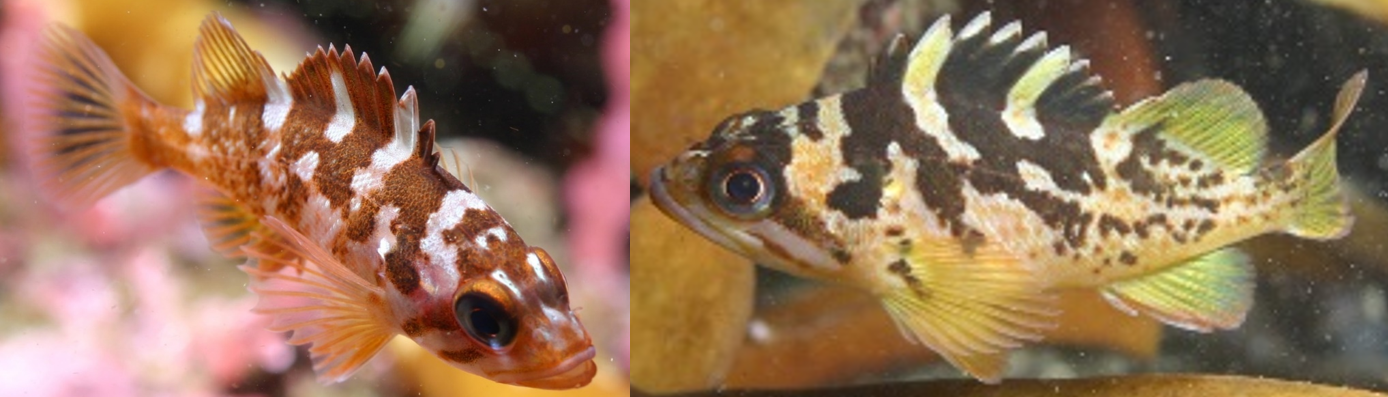
\includegraphics{cover_photo}~\\[1cm]
\pdftooltip{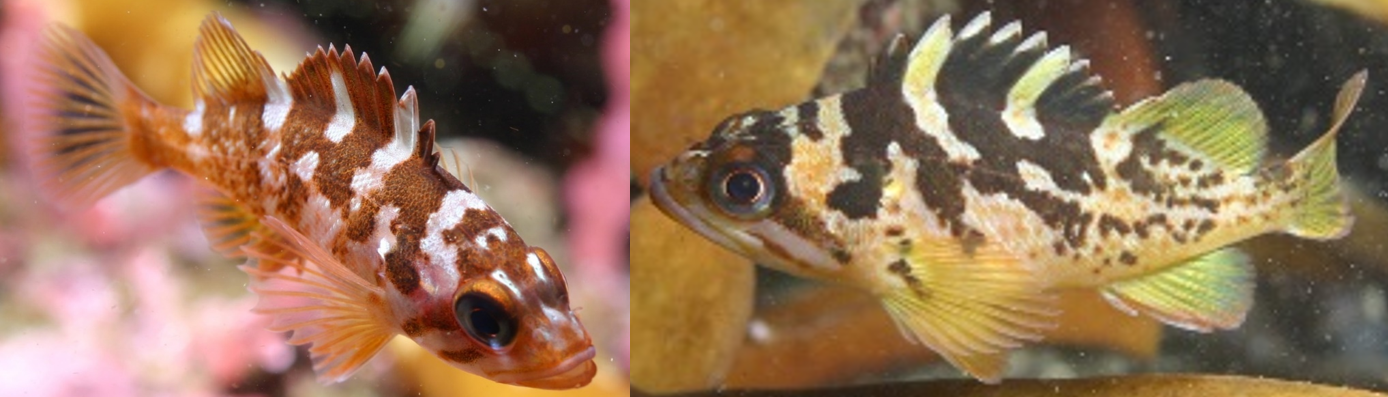
\includegraphics{cover_photo}}{This is a fish.}
Gopher rockfish (left) and black-and-yellow rockfish (right).      
\small
Photos by Steve Lonhart.

\vspace{.3cm}


Melissa H. Monk\textsuperscript{1}\\
Xi He\textsuperscript{1}\\

\vspace{.5cm}

\small
\textsuperscript{1}Southwest Fisheries Science Center, U.S. Department of Commerce, National Oceanic and Atmospheric Administration, National Marine Fisheries Service, 110 McAllister Way, Santa Cruz, California 95060\\

\vspace{1.5cm}


%\vfill
DRAFT SAFE\\
Disclaimer: This information is distributed solely for the purpose of pre-dissemination
peer review under applicable information quality guidelines. It has not been formally
disseminated by NOAA Fisheries. It does not represent and should not be construed to
represent any agency determination or policy. 

\vspace{.1cm}
%Bottom of the page
{\large \today}


\newpage{\thispagestyle{empty}}


\begin{flushleft}
This report may be cited as:

Monk, M. H.  and X. He. 2019. The Combined Status of Gopher (*Sebastes carnatus*) and Black-and-Yellow Rockfishes (*Sebastes chrysomelas*) in U.S. Waters Off California in 2019. Pacific Fishery Management Council, Portland, OR. Available from http://www.pcouncil.org/groundfish/stock-assessments/
\end{flushleft}

\maketitle

\pagenumbering{roman}
\setcounter{page}{1}
\end{center}

{
\setcounter{tocdepth}{4}
\tableofcontents
}
\setlength{\parskip}{5mm plus1mm minus1mm} \pagebreak

\setcounter{page}{1} \renewcommand{\thefigure}{\alph{figure}}
\renewcommand{\thetable}{\alph{table}}

\section*{Executive Summary}\label{executive-summary}
\addcontentsline{toc}{section}{Executive Summary}

\subsection*{Stock}\label{stock}
\addcontentsline{toc}{subsection}{Stock}

This assessment reports the status of the GBYR
(\emph{Sebastes carnatus/Sebastes chrysomelas}) resource in U.S. waters
off the coast of \ldots{} using data through 2018.

\subsection*{Catches}\label{catches}
\addcontentsline{toc}{subsection}{Catches}

Information on historical landings of GBYR are available back to
xxxx\ldots{} (Table \ref{tab:Exec_catch}). Commercial landings were
small during the years of World War II, ranging between 4 to 28 metric
tons (mt) per year.

(Figures \ref{fig:Exec_catch1}-\ref{fig:Exec_catch2})\\
(Figure \ref{fig:r4ss_catches})

Since 2000, annual total landings of GBYR have ranged between 70-168 mt,
with landings in 2018 totaling 91 mt.

\FloatBarrier

\begin{figure}
\centering
\includegraphics{Figures/rec_exec.png}
\caption{Catch history of GBYR for the recreational fleet.
\label{fig:Exec_catch1}}
\end{figure}

\begin{figure}
\centering
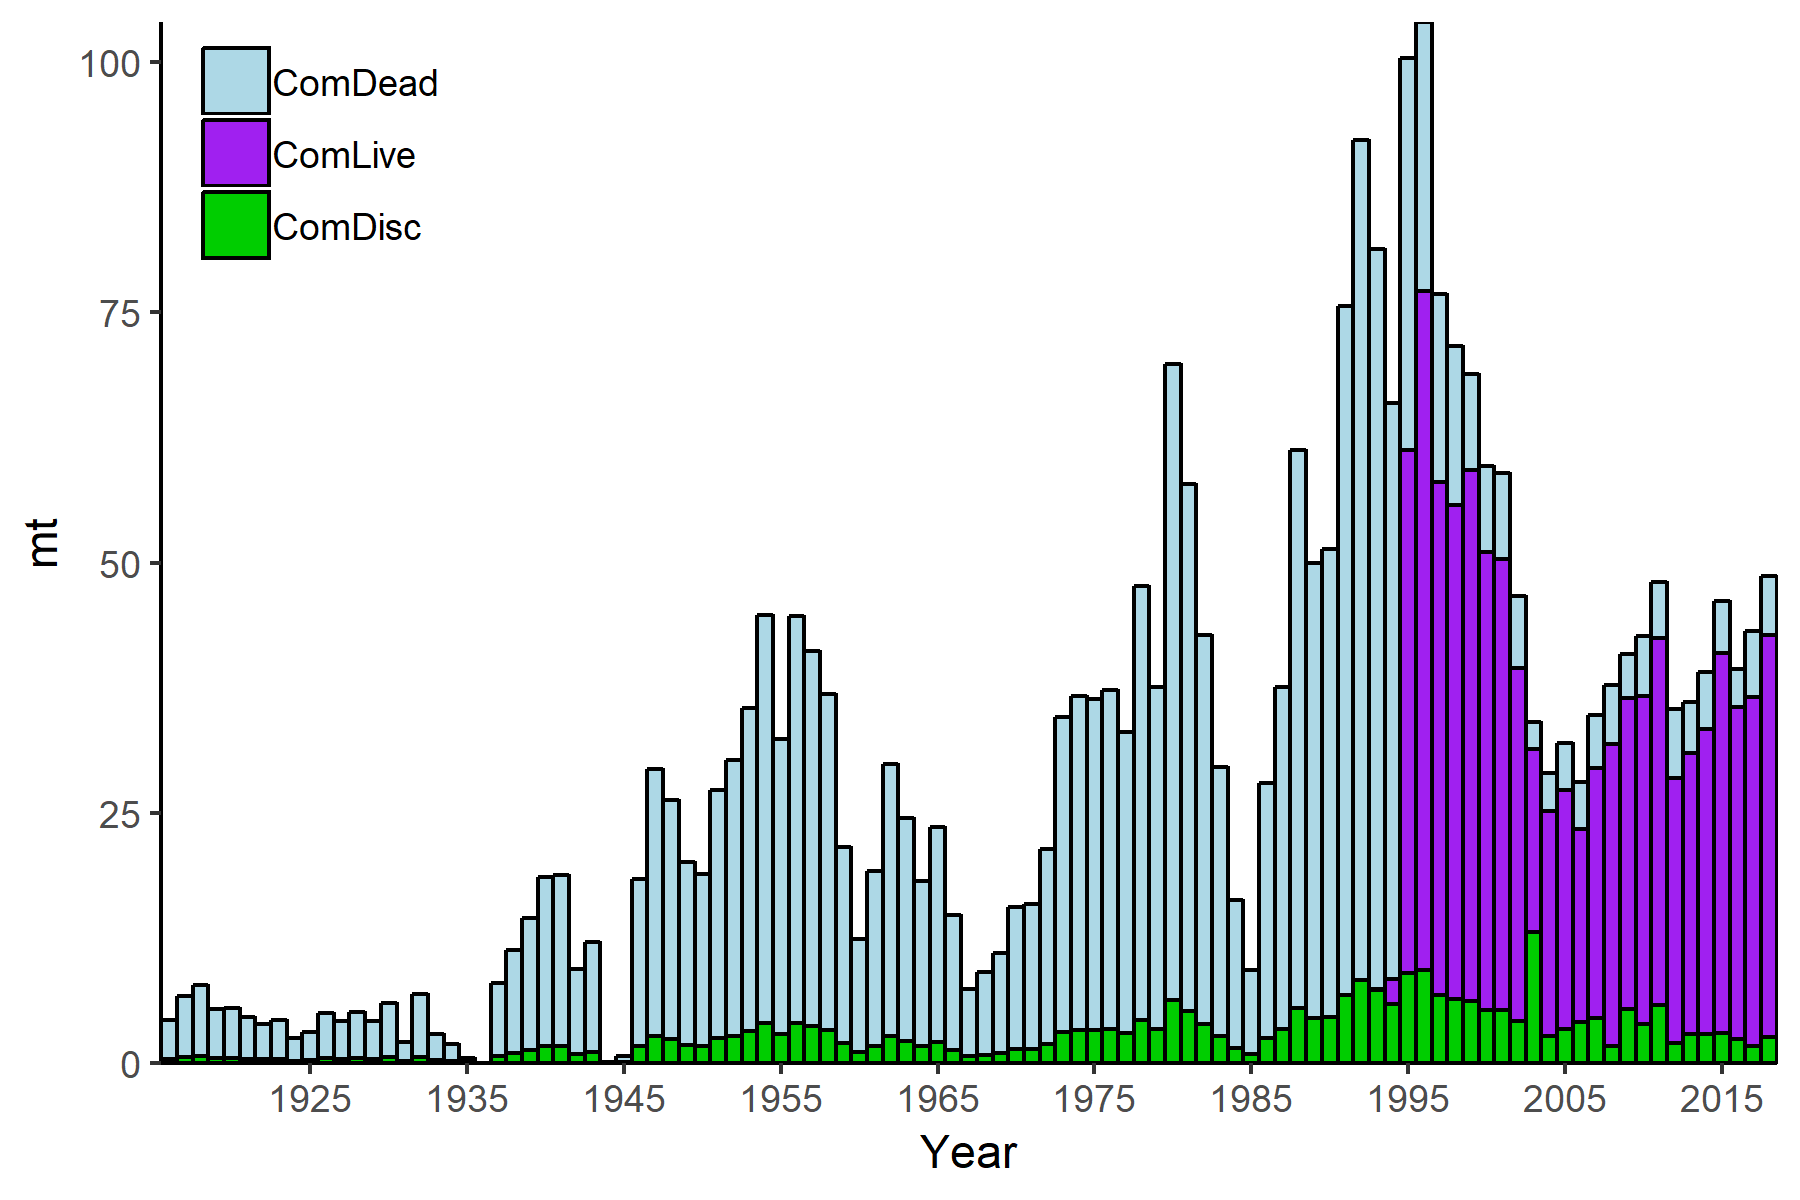
\includegraphics{Figures/comm_exec.png}
\caption{Catch history of GBYR for the commercial fleet by dead and live
landings, and discards. Catches in 1936 and 1946 were minimal.
\label{fig:Exec_catch2}}
\end{figure}

\FloatBarrier

\begin{figure}
\centering
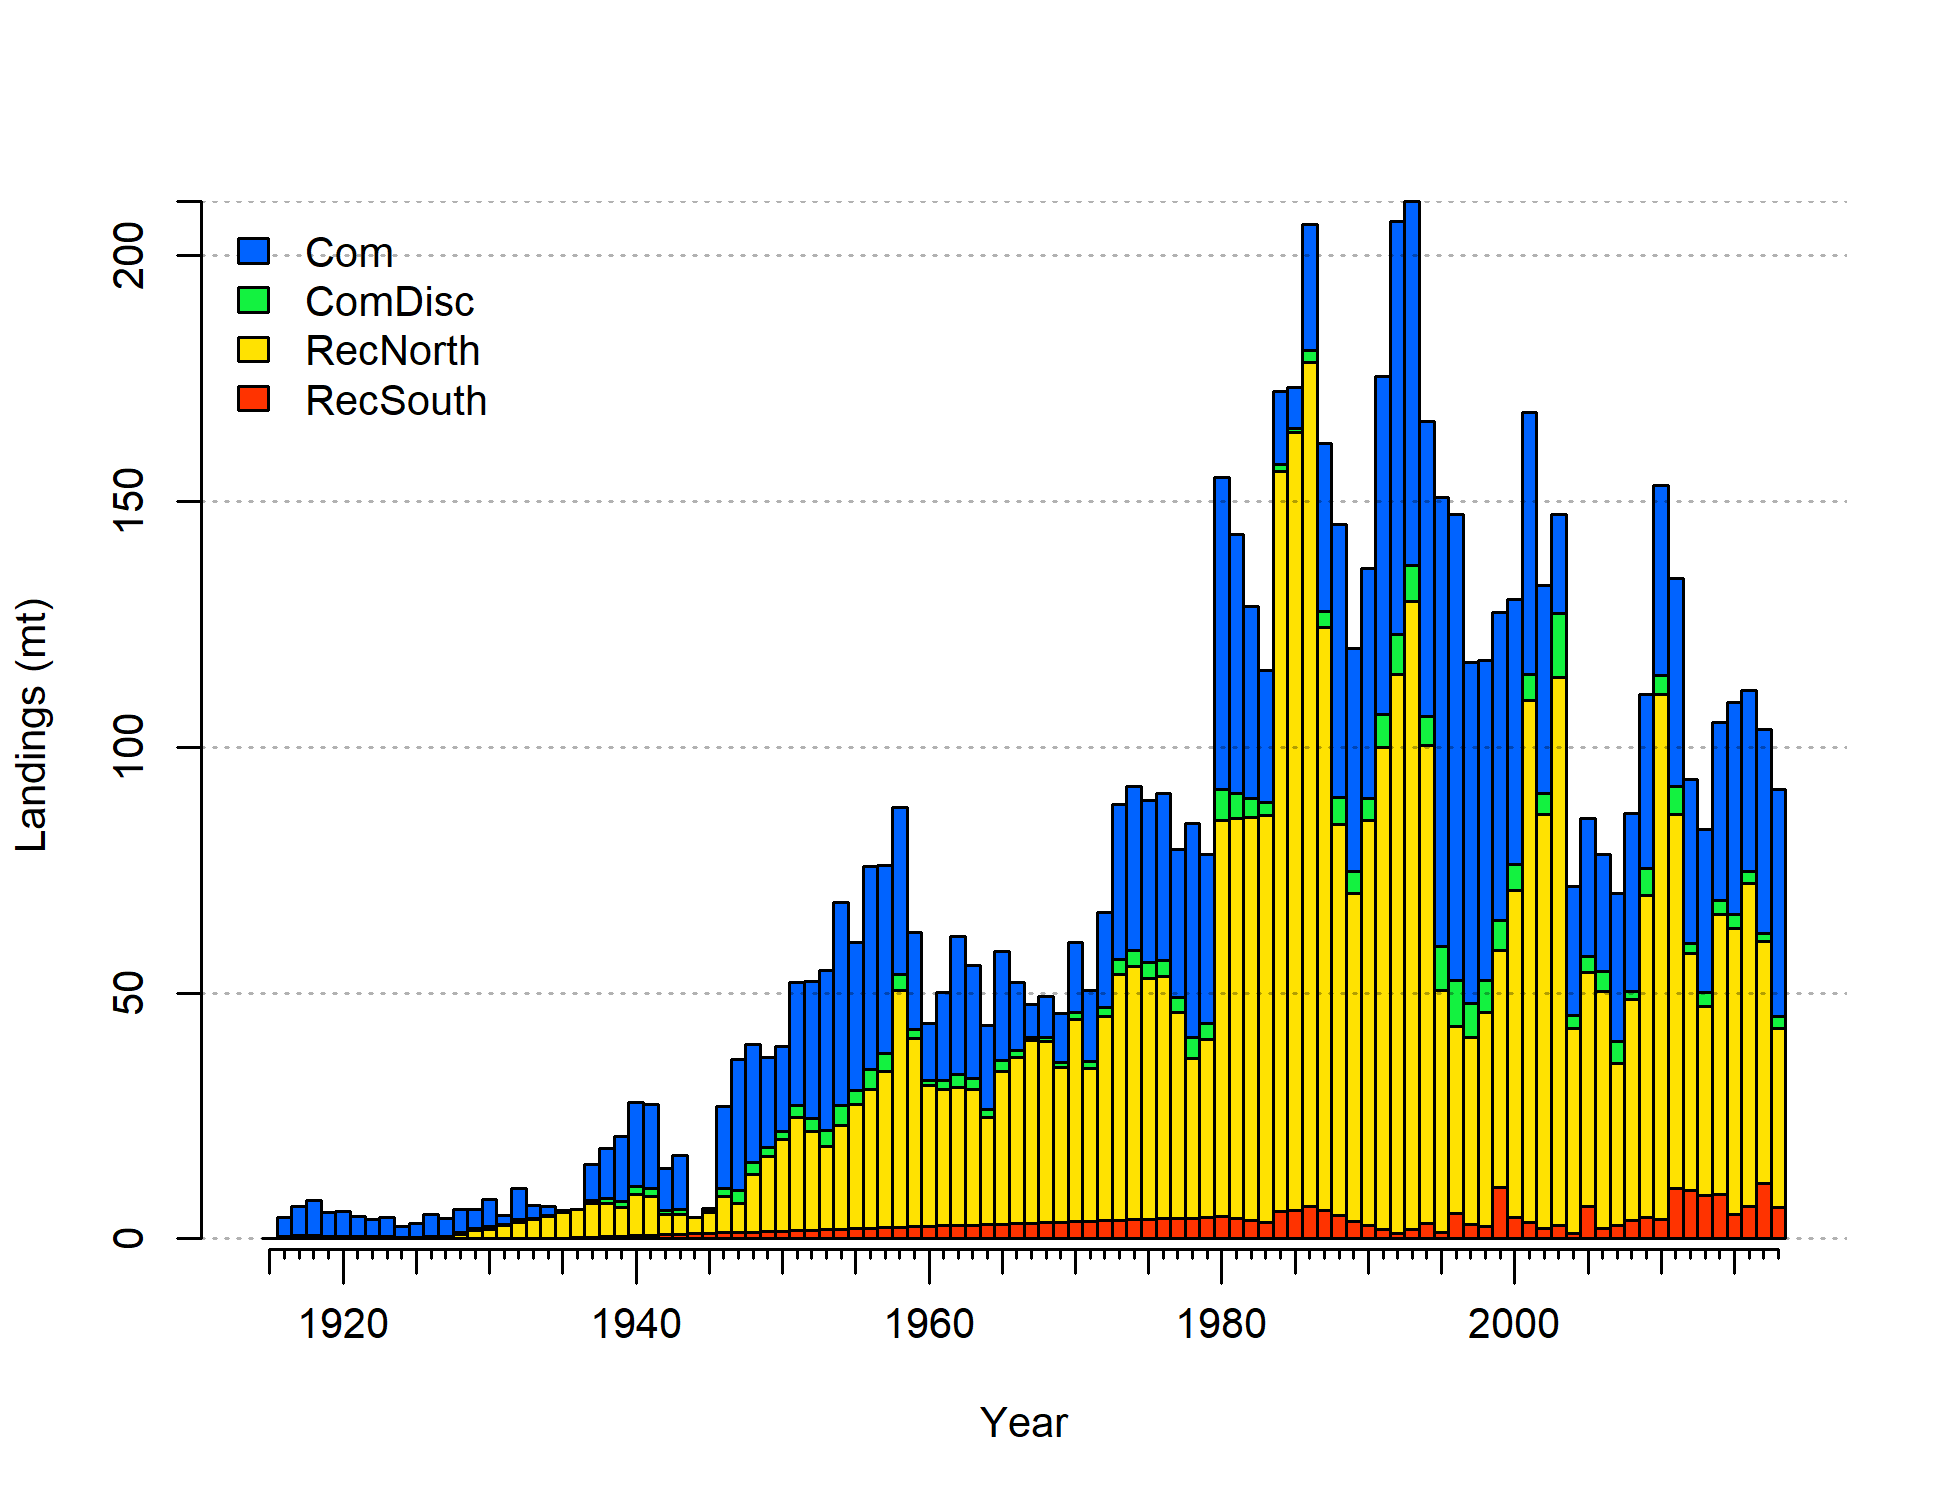
\includegraphics{r4ss/plots_mod1/catch2 landings stacked.png}
\caption{Catch history of GBYR in the model. \label{fig:r4ss_catches}}
\end{figure}

\begin{table}[ht]
\centering
\caption{Recent GBYR landings (mt) by 
                                            fleet.} 
\label{tab:Exec_catch}
\begin{tabular}{l>{\centering}p{1in}>{\centering}p{1in}>{\centering}p{1in}>{\centering}p{.9in}>{\centering}p{.9in}}
  \hline
Year & Commercial Retained & Commercial Discard & Recreational North & Recreational South & Total \\ 
  \hline
2009 & 35.42 & 5.38 & 65.64 & 4.30 & 110.73 \\ 
  2010 & 38.65 & 3.92 & 106.76 & 3.90 & 153.23 \\ 
  2011 & 42.28 & 5.72 & 76.16 & 10.24 & 134.41 \\ 
  2012 & 33.46 & 1.93 & 48.25 & 9.89 & 93.53 \\ 
  2013 & 33.17 & 2.85 & 38.43 & 8.86 & 83.30 \\ 
  2014 & 36.15 & 2.85 & 56.96 & 9.06 & 105.02 \\ 
  2015 & 43.18 & 2.93 & 58.09 & 5.00 & 109.20 \\ 
  2016 & 36.84 & 2.42 & 65.72 & 6.57 & 111.55 \\ 
  2017 & 41.51 & 1.65 & 49.36 & 11.15 & 103.66 \\ 
  2018 & 46.08 & 2.54 & 36.48 & 6.30 & 91.40 \\ 
   \hline
\end{tabular}
\end{table}

\FloatBarrier

\newpage

\subsection*{Data and Assessment}\label{data-and-assessment}
\addcontentsline{toc}{subsection}{Data and Assessment}

This a new full assessment for GBYR, which was last assessed in \ldots{}
using Stock Synthesis Version xx. This assessment uses the newest
version of Stock Synthesis (3.30.xx). The model begins in 1916, and
assumes the stock was at an unfished equilibrium that year.

(Figure \ref{fig:assess_region_map}).

\begin{figure}
\centering
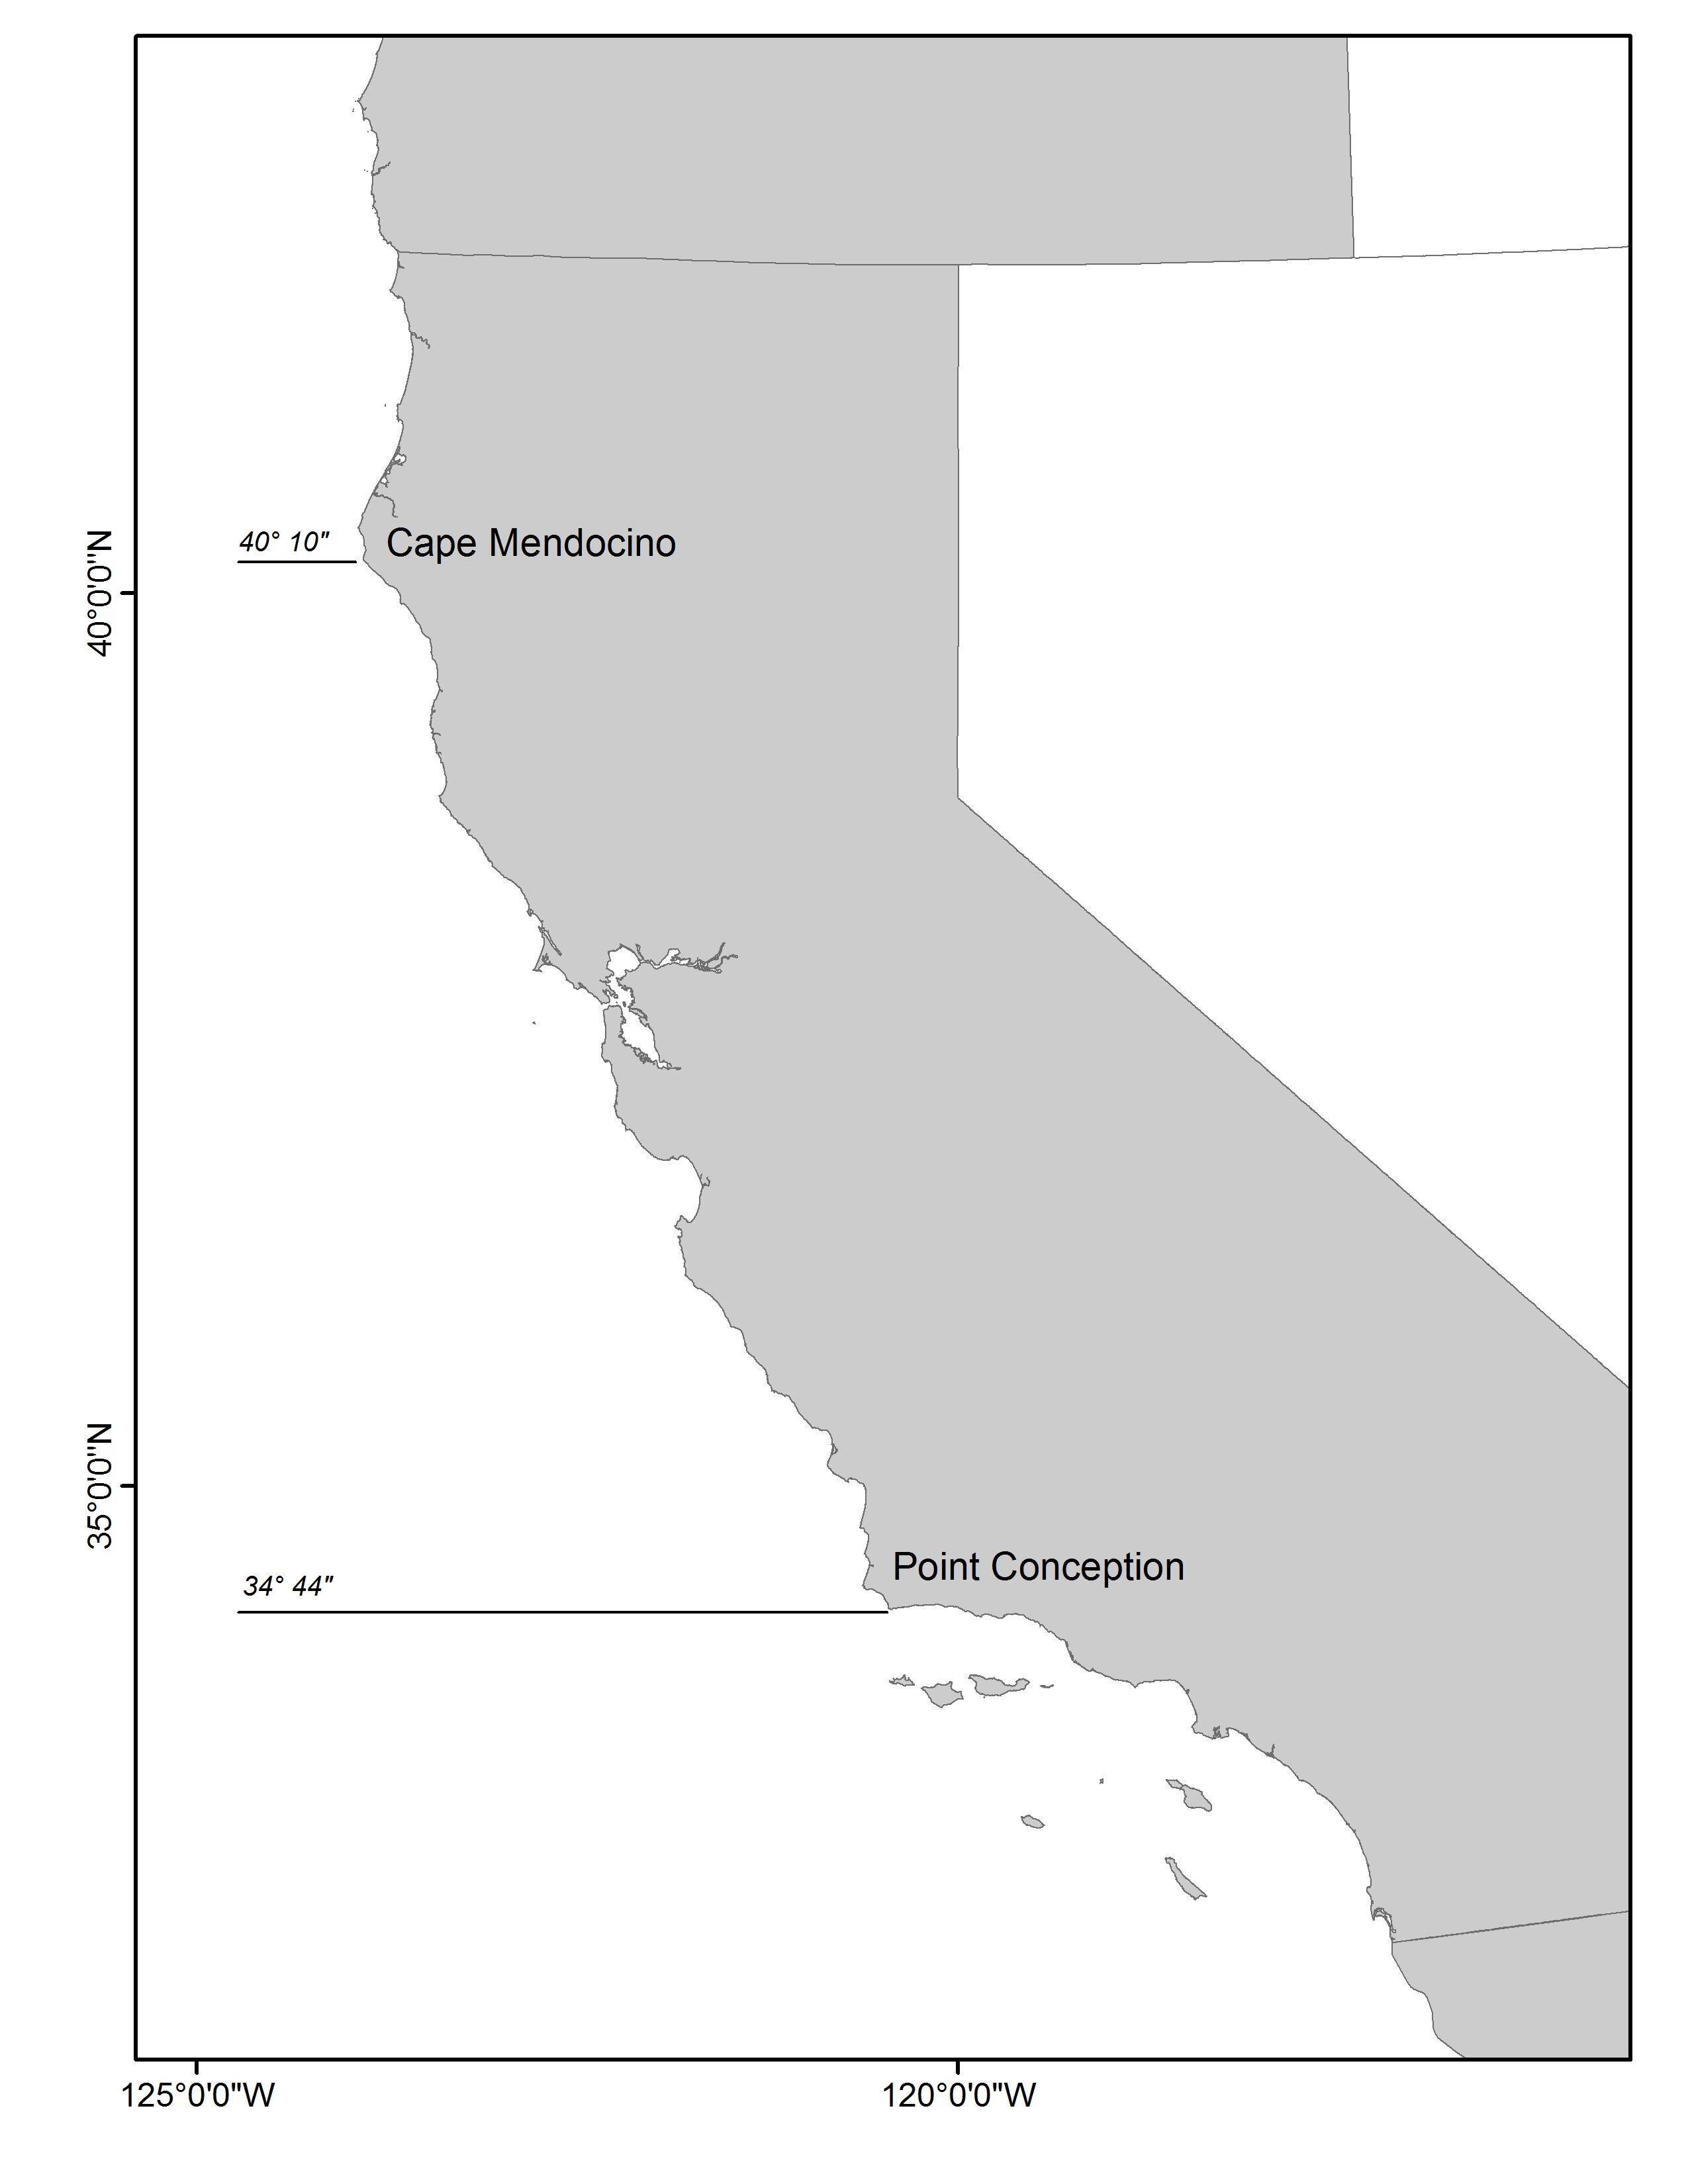
\includegraphics{Figures/assess_region_map.png}
\caption{Map depicting the core distribution of gopher and
black-and-yellow rockfishes. The stock assessment is bounded at Cape
Mendocino in the north to the U.S./Mexico border in the south.
\label{fig:assess_region_map}}
\end{figure}

\FloatBarrier

\subsection*{Stock Biomass}\label{stock-biomass}
\addcontentsline{toc}{subsection}{Stock Biomass}

(Figure \ref{fig:Spawnbio_all} and Table
\ref{tab:SpawningDeplete_mod1}).

The 2018 estimated spawning biomass relative to unfished equilibrium
spawning biomass is above the target of 40\% of unfished spawning
biomass at 4 520\% (95\% asymptotic interval: \(\pm\) 2 340\% - 6 700\%)
(Figure \ref{fig:RelDeplete_all}). Approximate confidence intervals
based on the asymptotic variance estimates show that the uncertainty in
the estimated spawning biomass is high.

\FloatBarrier

\begin{table}[ht]
\centering
\caption{Recent trend in beginning of the 
                                      year spawning output and depletion for
                                      the model for GBYR.} 
\label{tab:SpawningDeplete_mod1}
\begin{tabular}{l>{\centering}p{1.3in}>{\centering}p{1.2in}>{\centering}p{1in}>{\centering}p{1.2in}}
  \hline
Year & Spawning Output (million eggs) & \~{} 95\% confidence interval & Estimated depletion & \~{} 95\% confidence interval \\ 
  \hline
2010 & 877 & 550 - 1205 & 63.33 & 45.67 - 80.98 \\ 
  2011 & 805 & 497 - 1113 & 58.07 & 41.64 - 74.5 \\ 
  2012 & 745 & 454 - 1036 & 53.76 & 38.39 - 69.13 \\ 
  2013 & 712 & 434 - 990 & 51.37 & 36.9 - 65.84 \\ 
  2014 & 688 & 420 - 957 & 49.67 & 35.88 - 63.45 \\ 
  2015 & 658 & 395 - 921 & 47.49 & 34.08 - 60.9 \\ 
  2016 & 634 & 372 - 895 & 45.73 & 32.37 - 59.08 \\ 
  2017 & 616 & 351 - 880 & 44.43 & 30.83 - 58.03 \\ 
  2018 & 611 & 338 - 884 & 44.08 & 29.93 - 58.22 \\ 
  2019 & 626 & 332 - 919 & 45.17 & 23.35 - 66.98 \\ 
   \hline
\end{tabular}
\end{table}

\FloatBarrier

\begin{figure}
\centering
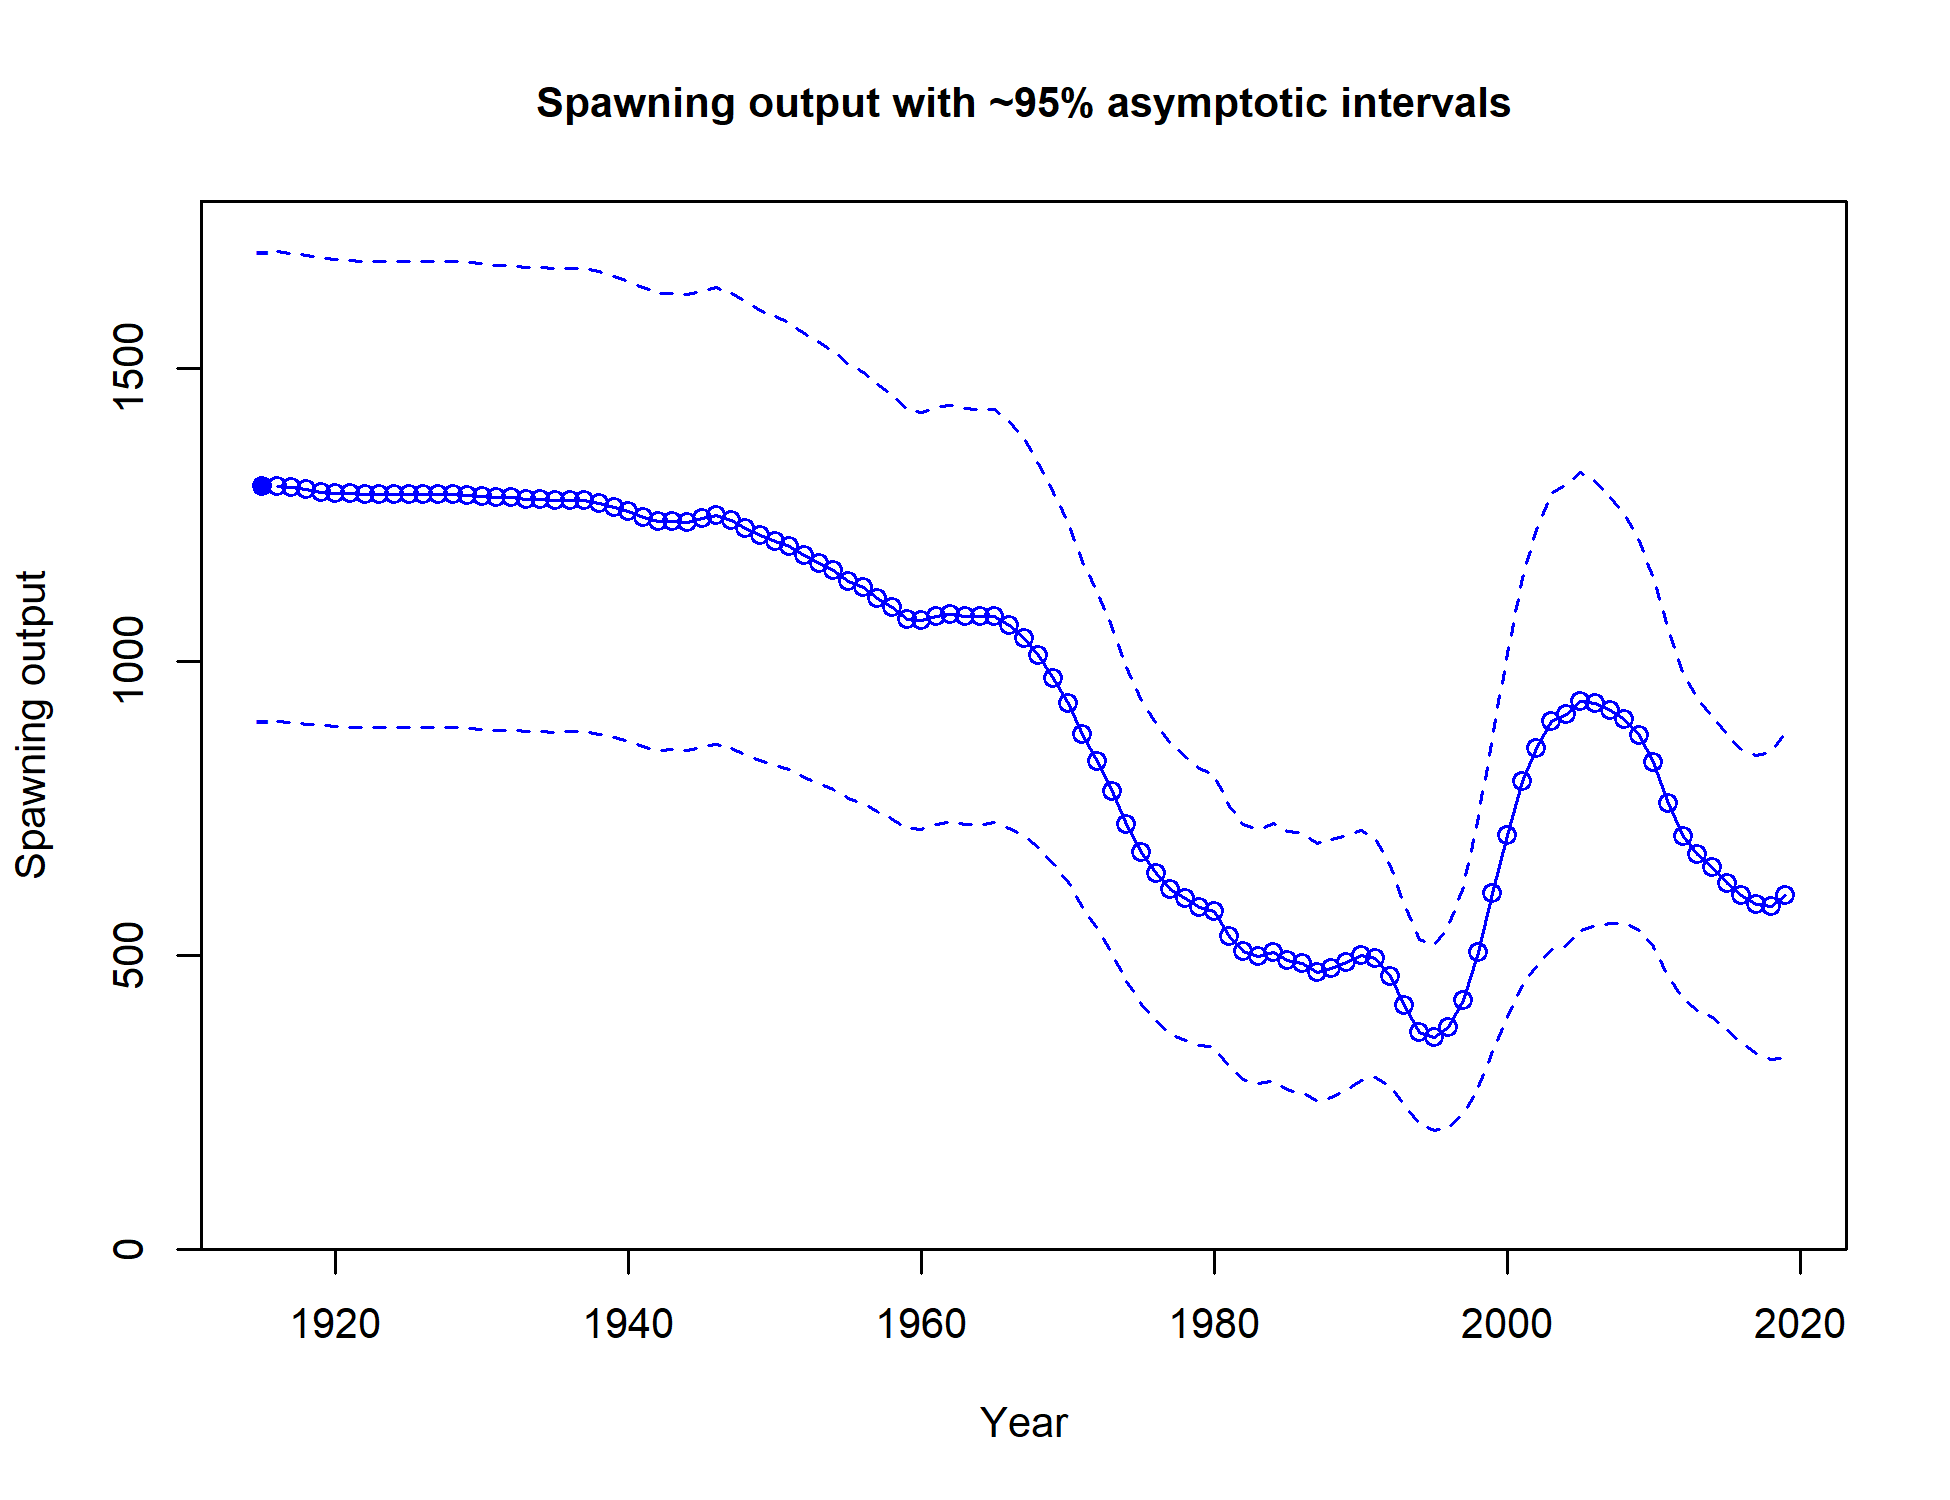
\includegraphics{r4ss/plots_mod1/ts7_Spawning_output_with_95_asymptotic_intervals_intervals.png}
\caption{Time series of spawning biomass trajectory (circles and line:
median; light broken lines: 95\% credibility intervals) for the base
case assessment model. \label{fig:Spawnbio_all}}
\end{figure}

\begin{figure}
\centering
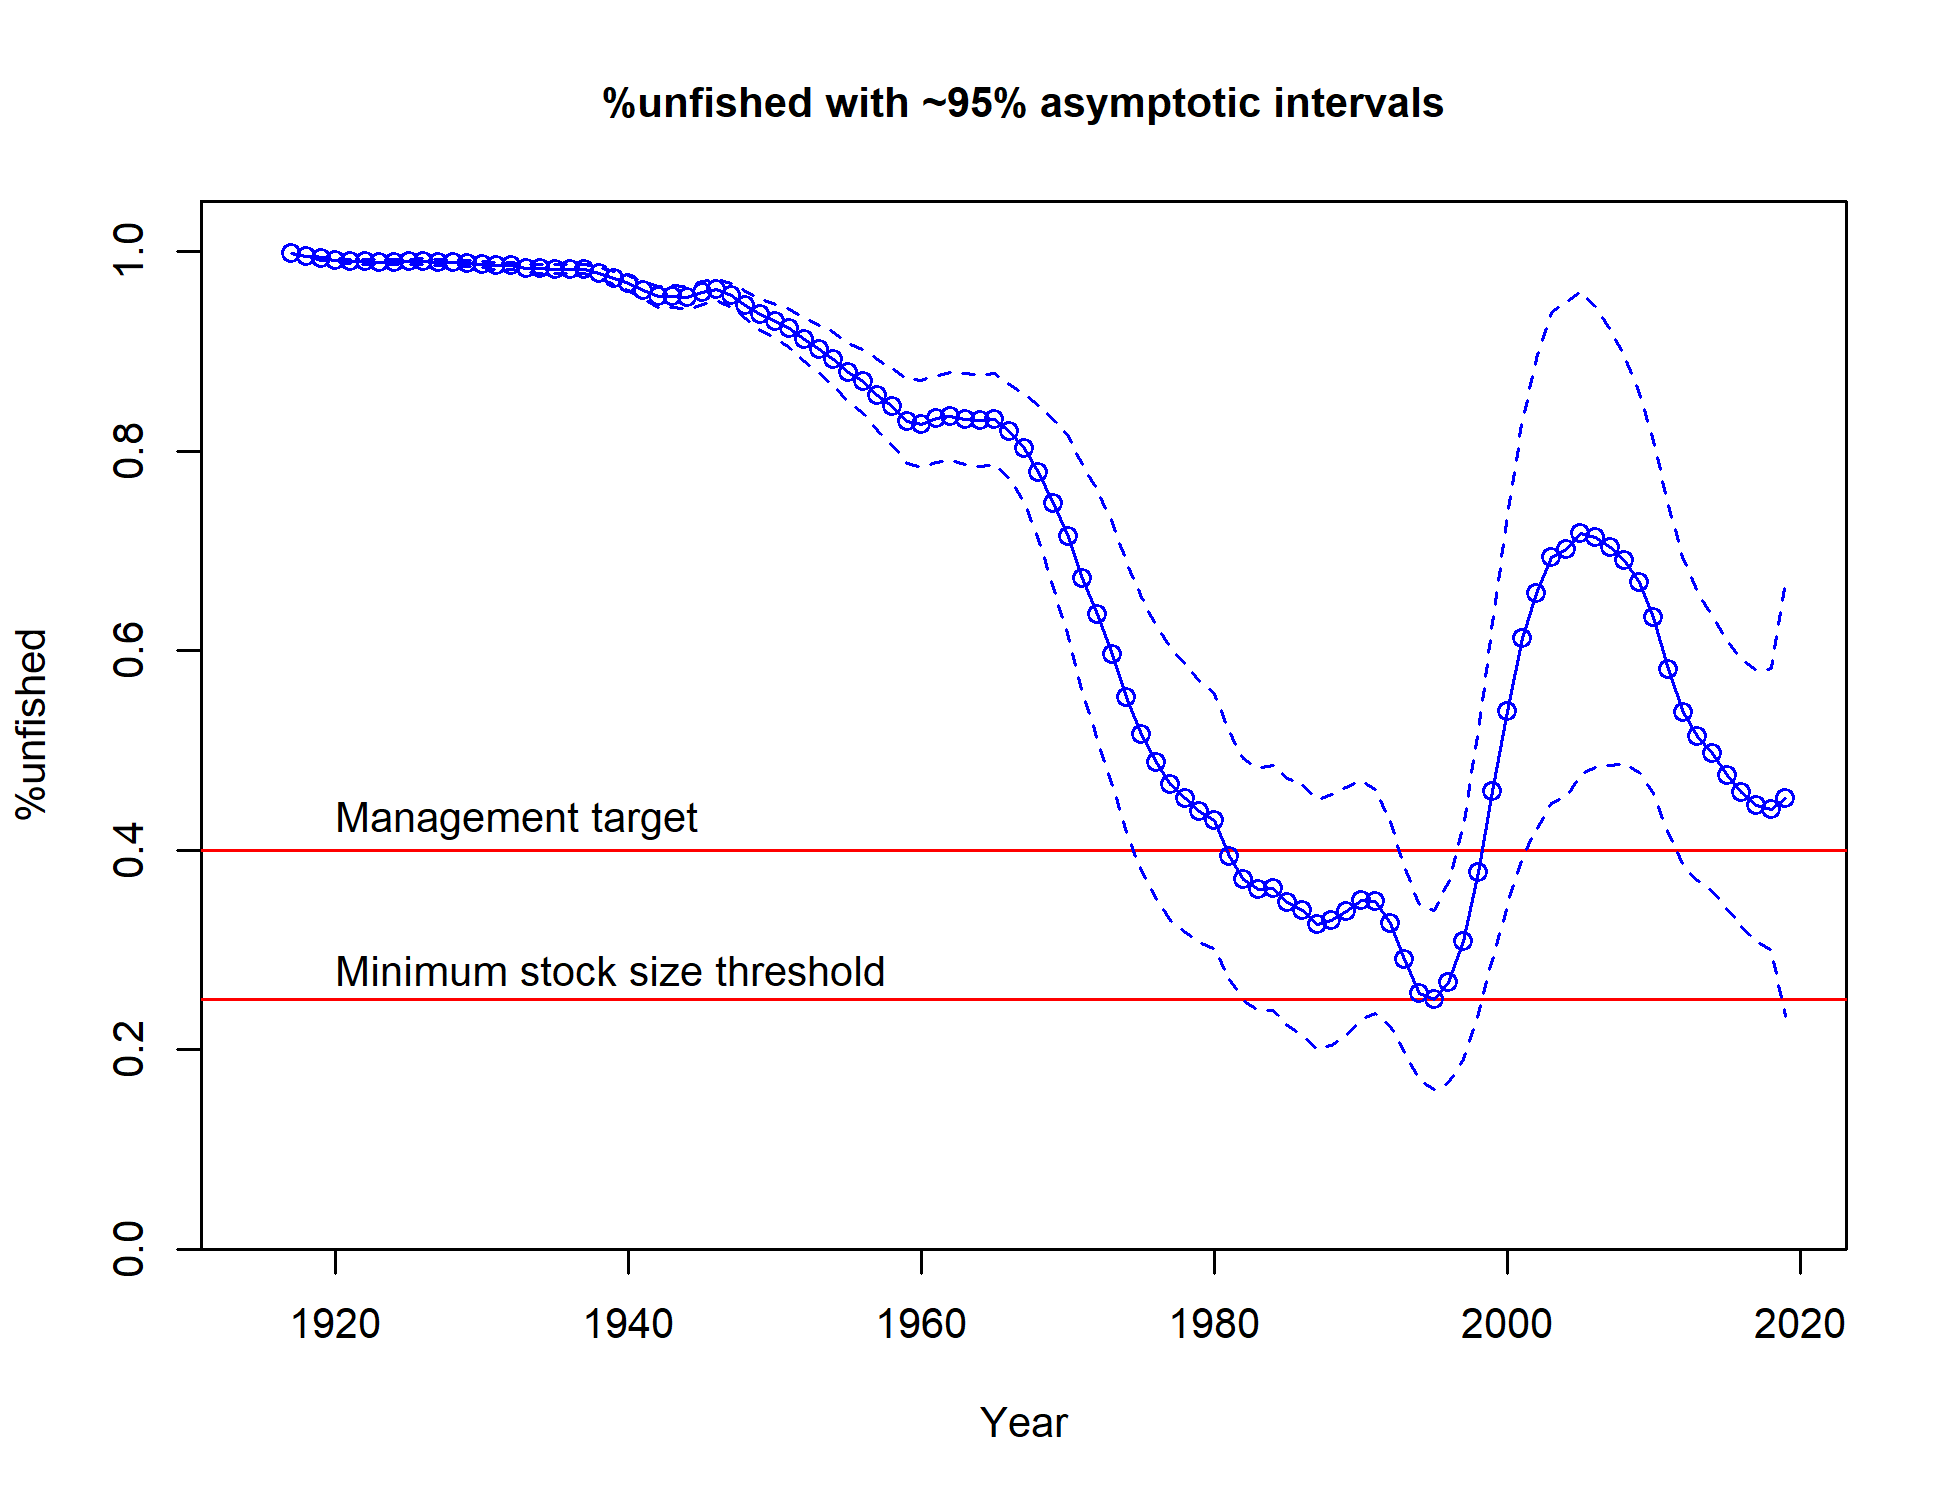
\includegraphics{r4ss/plots_mod1/ts9_unfished_with_95_asymptotic_intervals_intervals.png}
\caption{Estimated percent depletion with approximate 95\% asymptotic
confidence intervals (dashed lines) for the base case assessment model.
\label{fig:RelDeplete_all}}
\end{figure}

\FloatBarrier

\subsection*{Recruitment}\label{recruitment}
\addcontentsline{toc}{subsection}{Recruitment}

Recruitment deviations were estimated from xxxx-xxxx (Figure
\ref{fig:Recruits_all} and Table \ref{tab:Recruit_mod1}).

\begin{table}[ht]
\centering
\caption{Recent recruitment for the GBYR assessment.} 
\label{tab:Recruit_mod1}
\begin{tabular}{>{\centering}p{.8in}>{\centering}p{1.6in}>{\centering}p{1.6in}}
  \hline
Year & Estimated Recruitment (1,000s) & \~{} 95\% confidence interval \\ 
  \hline
2010 & 3817 & 1496 - 9738 \\ 
  2011 & 3564 & 1358 - 9354 \\ 
  2012 & 3610 & 1346 - 9679 \\ 
  2013 & 4355 & 1619 - 11711 \\ 
  2014 & 6351 & 2368 - 17032 \\ 
  2015 & 8323 & 3082 - 22476 \\ 
  2016 & 7554 & 2745 - 20791 \\ 
  2017 & 5963 & 2111 - 16842 \\ 
  2018 & 4790 & 1661 - 13814 \\ 
  2019 & 4789 & 1610 - 14244 \\ 
   \hline
\end{tabular}
\end{table}

\FloatBarrier

\begin{figure}
\centering
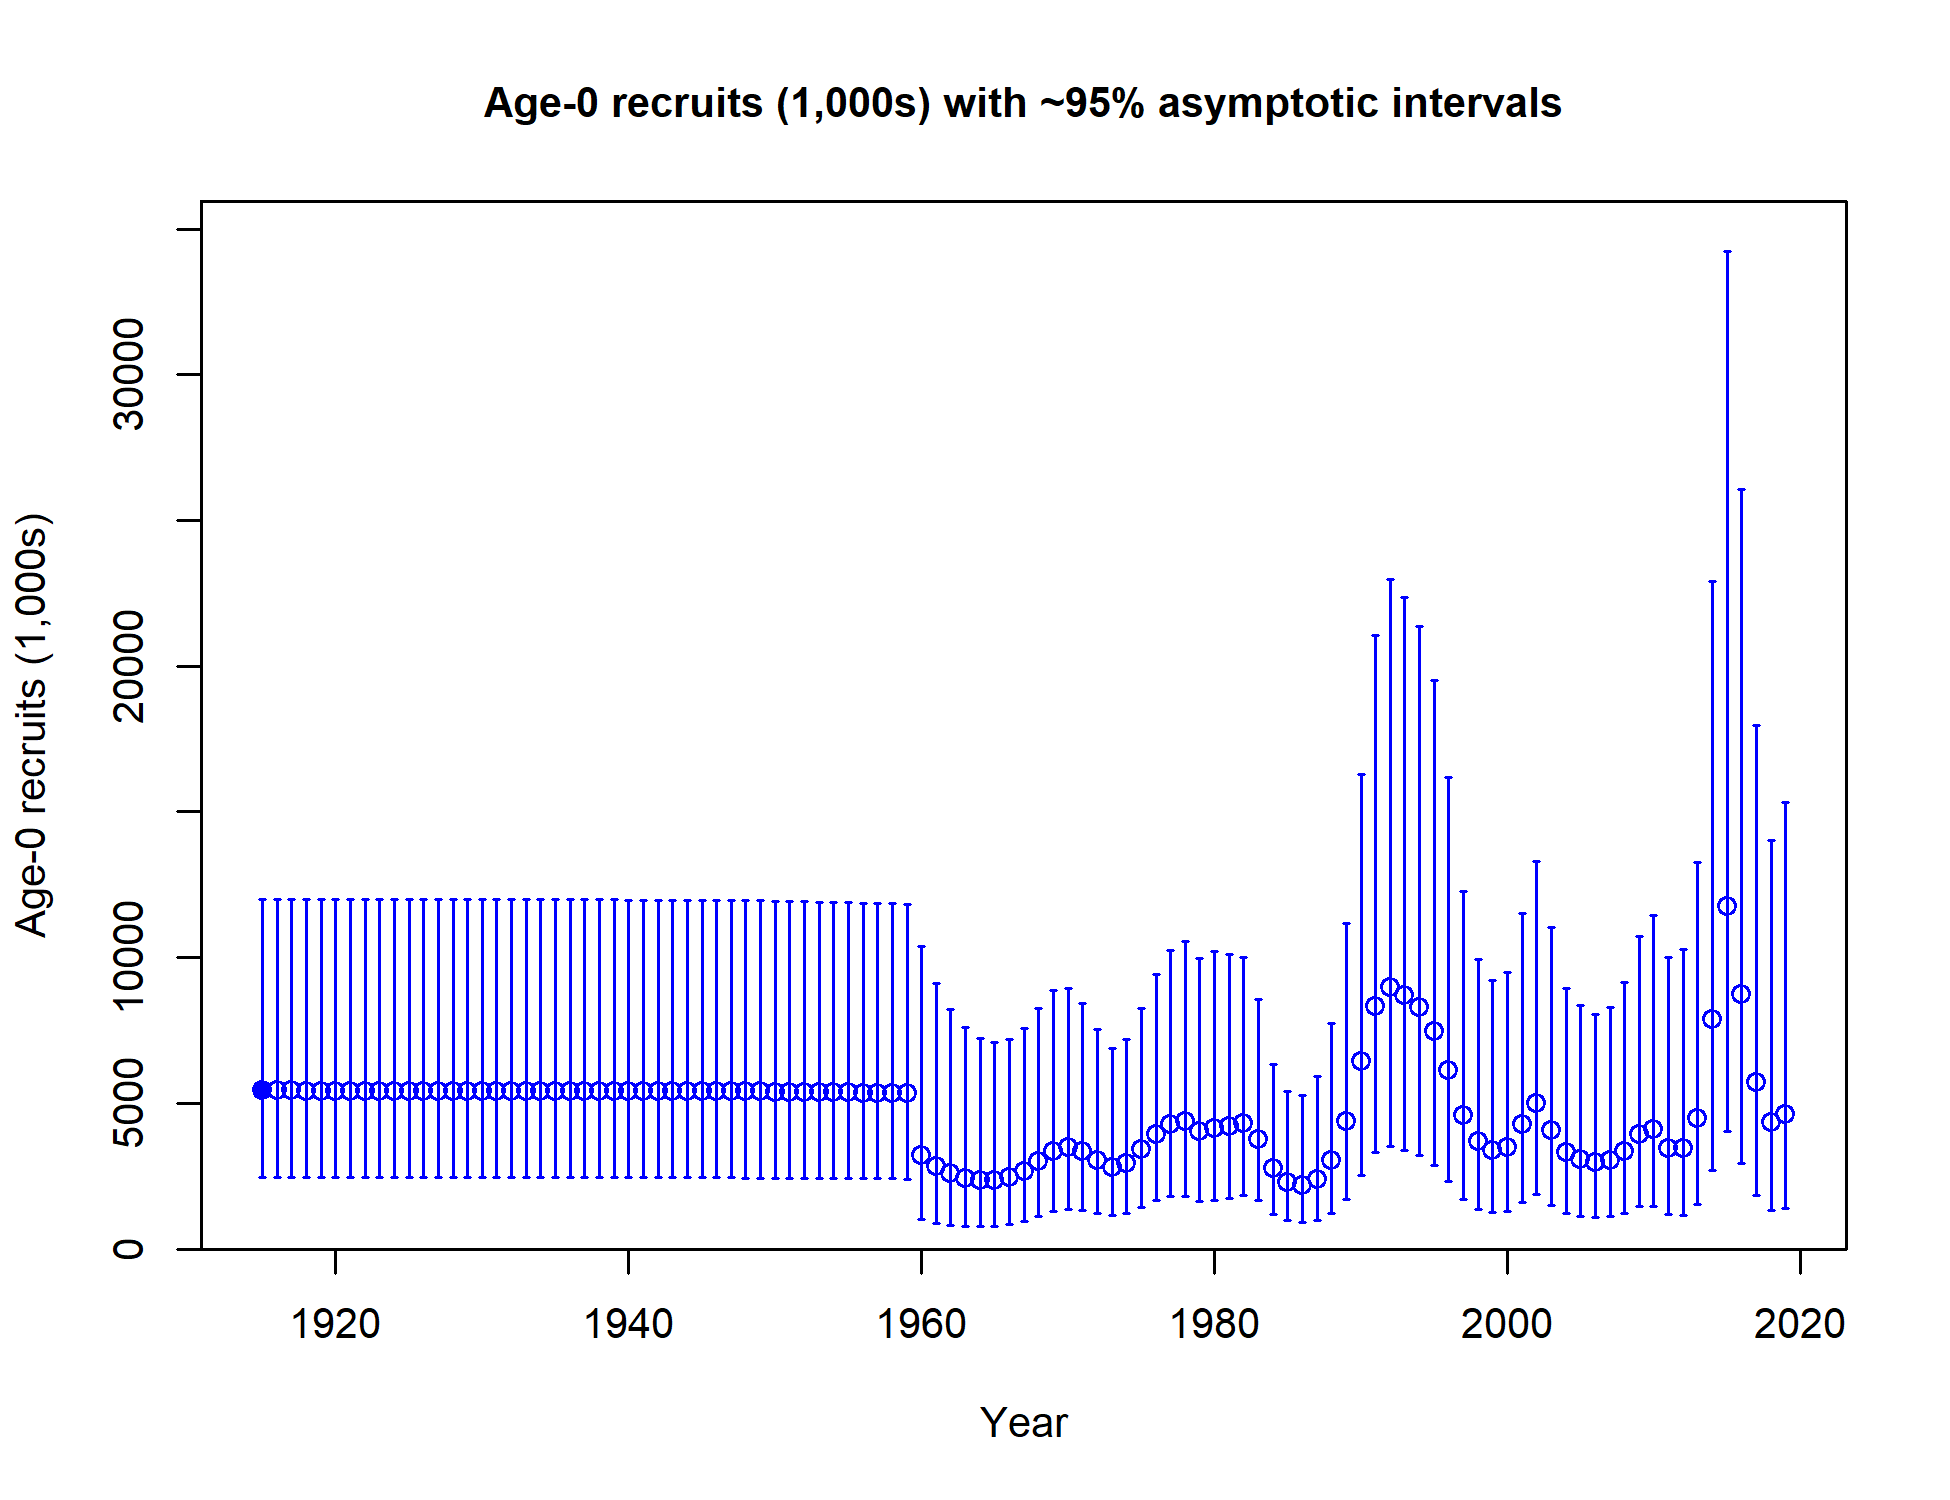
\includegraphics{r4ss/plots_mod1/ts11_Age-0_recruits_(1000s)_with_95_asymptotic_intervals.png}
\caption{Time series of estimated GBYR recruitments for the base-case
model with 95\% confidence or credibility intervals.
\label{fig:Recruits_all}}
\end{figure}

\FloatBarrier

\subsection*{Exploitation status}\label{exploitation-status}
\addcontentsline{toc}{subsection}{Exploitation status}

Harvest rates estimated by the base model \ldots{}.. management target
levels (Table \ref{tab:SPR_Exploit_mod1} and Figure \ref{fig:SPR_all}).

\FloatBarrier

\begin{table}[ht]
\centering
\caption{Recent trend in spawning potential 
                                        ratio and exploitation for GBYR in the model.  Fishing intensity is (1-SPR) 
                                        divided by 50\% (the SPR target) and exploitation 
                                        is F divided by F\textsubscript{SPR}.} 
\label{tab:SPR_Exploit_mod1}
\begin{tabular}{l>{\centering}p{1in}>{\centering}p{1.2in}>{\centering}p{1in}>{\centering}p{1.2in}}
  \hline
Year & Fishing intensity & \~{} 95\% confidence interval & Exploitation rate & \~{} 95\% confidence interval \\ 
  \hline
2009 & 0.60 & 0.37 - 0.82 & 0.07 & 0.05 - 0.1 \\ 
  2010 & 0.74 & 0.49 - 0.98 & 0.11 & 0.07 - 0.15 \\ 
  2011 & 0.73 & 0.48 - 0.98 & 0.10 & 0.06 - 0.14 \\ 
  2012 & 0.62 & 0.39 - 0.86 & 0.07 & 0.05 - 0.1 \\ 
  2013 & 0.60 & 0.37 - 0.83 & 0.07 & 0.04 - 0.09 \\ 
  2014 & 0.70 & 0.45 - 0.95 & 0.09 & 0.05 - 0.12 \\ 
  2015 & 0.73 & 0.48 - 0.99 & 0.09 & 0.05 - 0.13 \\ 
  2016 & 0.77 & 0.5 - 1.03 & 0.09 & 0.05 - 0.13 \\ 
  2017 & 0.76 & 0.49 - 1.03 & 0.08 & 0.04 - 0.12 \\ 
  2018 & 0.72 & 0.45 - 0.98 & 0.07 & 0.03 - 0.1 \\ 
   \hline
\end{tabular}
\end{table}

\FloatBarrier

\begin{figure}
\centering
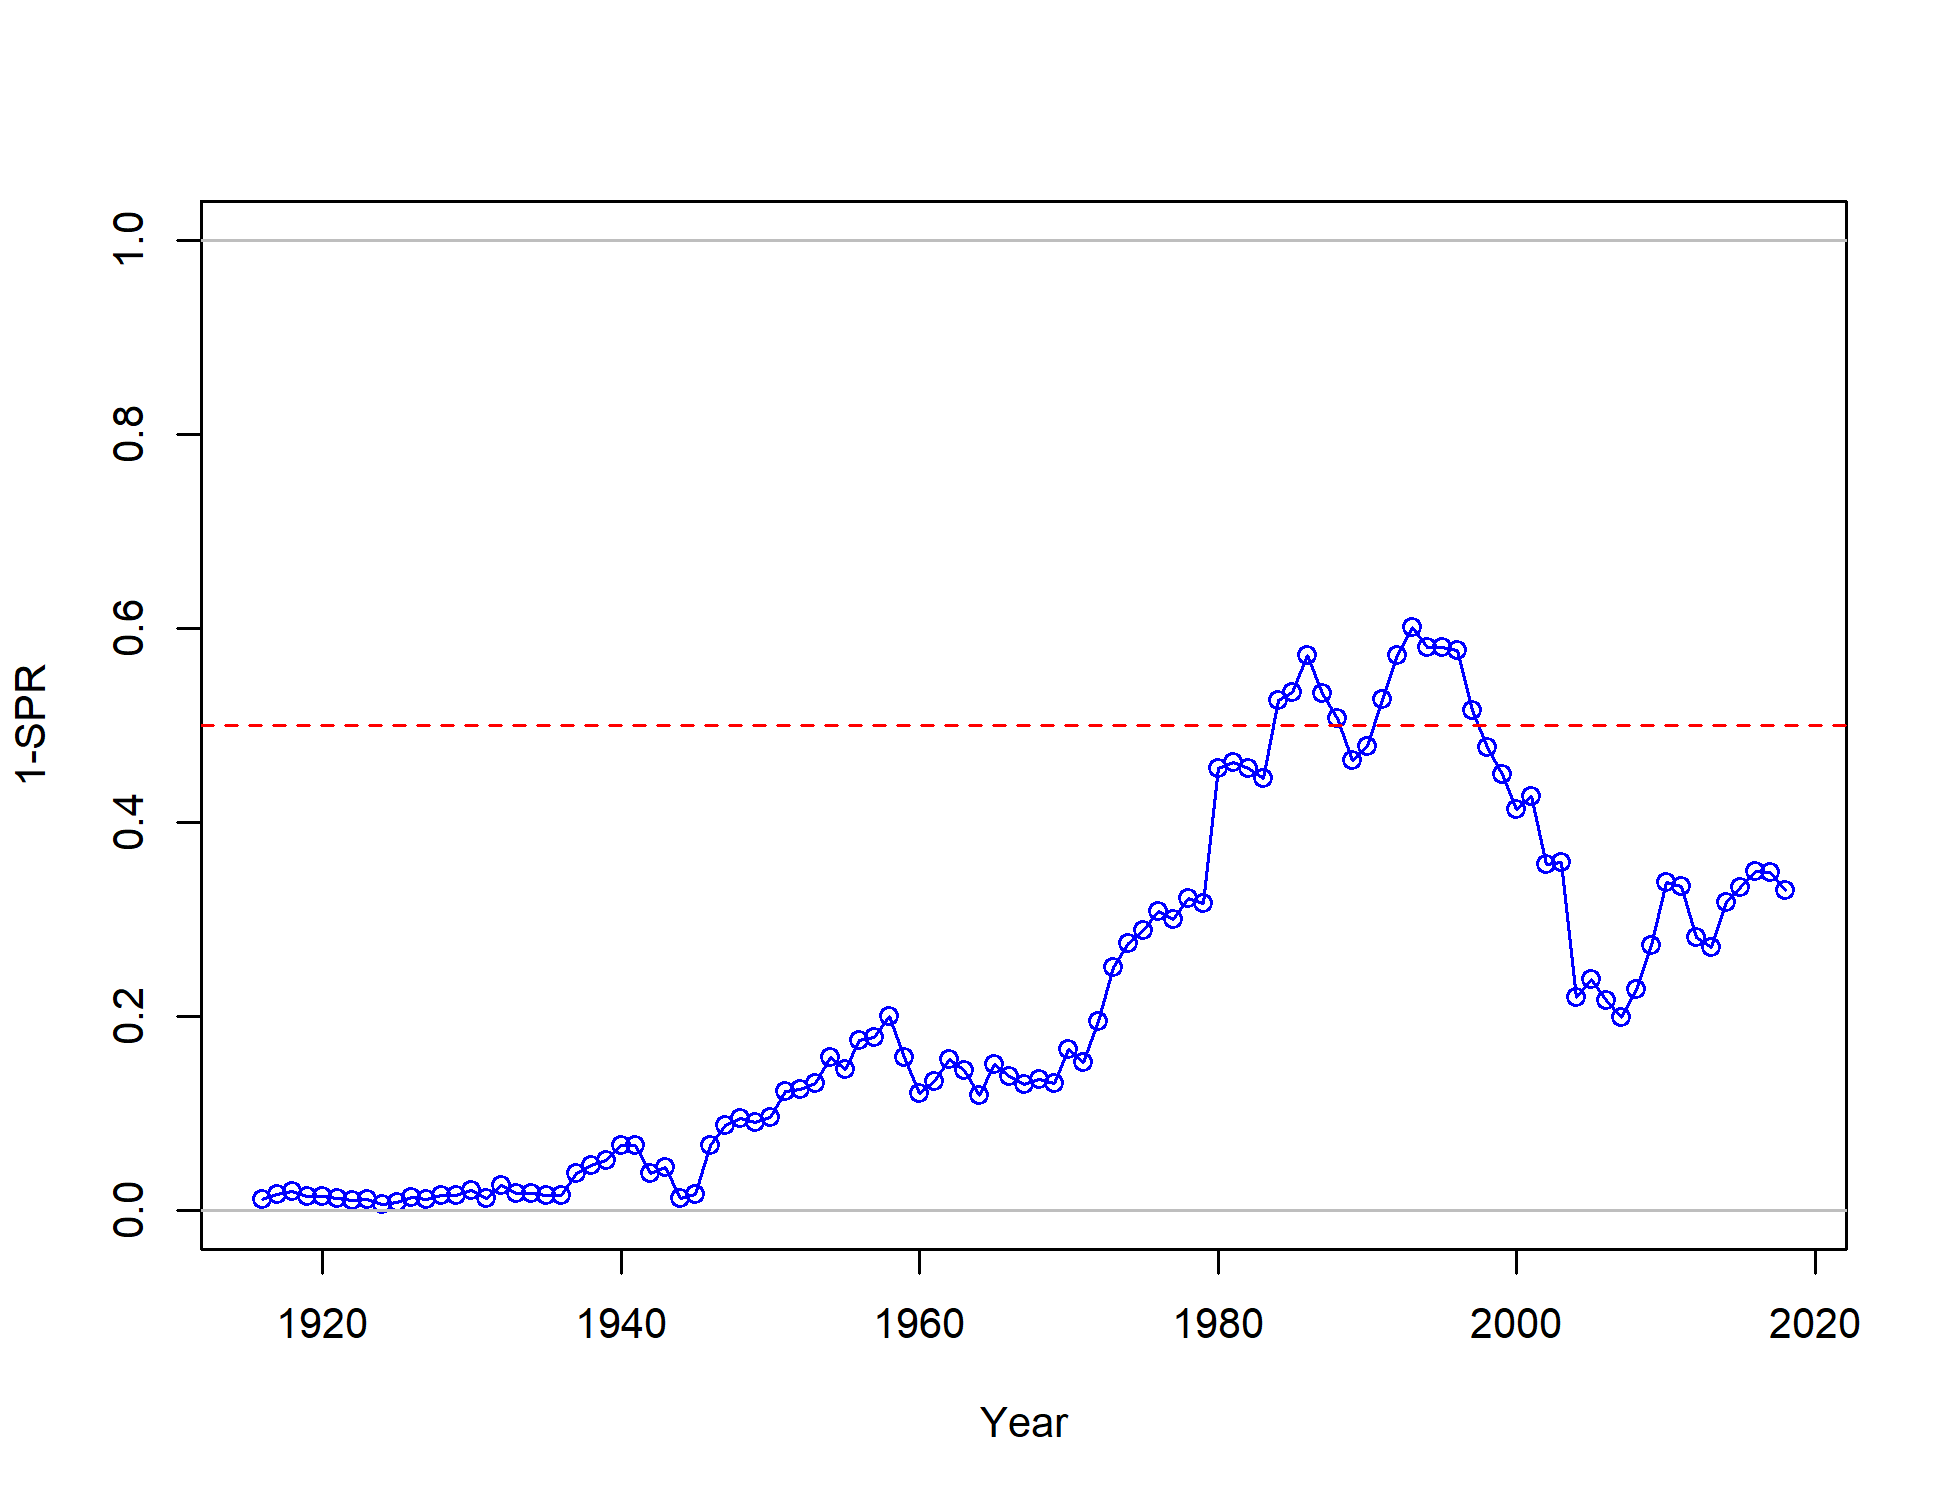
\includegraphics{r4ss/plots_mod1/SPR2_minusSPRseries.png}
\caption{Estimated spawning potential ratio (SPR) for the base-case
model. One minus SPR is plotted so that higher exploitation rates occur
on the upper portion of the y-axis. The management target is plotted as
a red horizontal line and values above this reflect harvests in excess
of the overfishing proxy based on the SPR\textsubscript{50\%} harvest
rate. The last year in the time series is 2018. \label{fig:SPR_all}}
\end{figure}

\FloatBarrier

\subsection*{Ecosystem Considerations}\label{ecosystem-considerations}
\addcontentsline{toc}{subsection}{Ecosystem Considerations}

In this assessment, ecosystem considerations were not explicitly
included in the analysis.\\
This is primarily due to a lack of relevant data and results of analyses
(conducted elsewhere) that could contribute ecosystem-related
quantitative information for the assessment.

\subsection*{Reference Points}\label{reference-points}
\addcontentsline{toc}{subsection}{Reference Points}

This stock assessment estimates that GBYR in the model is above the
biomass target (\(SB_{40\%}\)), and well above the minimum stock size
threshold (\(SB_{25\%}\)). The estimated relative depletion level for
the base model in 2019 is 4 520\% (95\% asymptotic interval: \(\pm\) 2
340\% - 6 700\%, corresponding to an unfished spawning biomass of 626
million eggs (95\% asymptotic interval: 332 - 919 million eggs) of
spawning biomass in the base model (Table \ref{tab:Ref_pts_mod1}).
Unfished age 1+ biomass was estimated to be 2,206 mt in the base case
model. The target spawning biomass (\(SB_{40\%}\)) is 554 million eggs,
which corresponds with an equilibrium yield of 181 mt. Equilibrium yield
at the proxy \(F_{MSY}\) harvest rate corresponding to \(SPR_{50\%}\) is
169 mt (Figure \ref{fig:Yield_all}).

\FloatBarrier

\begin{table}[ht]
\centering
\caption{Summary of reference 
                                      points and management quantities for the 
                                      base case model.} 
\label{tab:Ref_pts_mod1}
\begin{tabular}{>{\raggedright}p{4.1in}>{\raggedleft}p{.62in}>{\raggedleft}p{.62in}>{\raggedleft}p{.62in}}
  \hline
\textbf{Quantity} & \textbf{Estimate} & \textbf{Low 2.5\%  limit} & \textbf{High 2.5\%  limit} \\ 
  \hline
Unfished spawning output (million eggs) & 1,386 & 997 & 1,774 \\ 
  Unfished age 1+ biomass (mt) & 2,206 & 1,701 & 2,710 \\ 
  Unfished recruitment ($R_{0}$) & 5,057 & 1,156 & 8,958 \\ 
  Spawning output(2018 million eggs) & 611 & 338 & 884 \\ 
  Depletion (2018) & 0.441 & 0.299 & 0.582 \\ 
  \textbf{$\text{Reference points based on } \mathbf{SB_{40\%}}$} &  &  &  \\ 
  Proxy spawning output ($B_{40\%}$) & 554 & 449 & 659 \\ 
  SPR resulting in $B_{40\%}$ ($SPR_{B40\%}$) & 0.458 & 0.458 & 0.458 \\ 
  Exploitation rate resulting in $B_{40\%}$ & 0.151 & 0.109 & 0.194 \\ 
  Yield with $SPR_{B40\%}$ at $B_{40\%}$ (mt) & 181 & 110 & 252 \\ 
  \textbf{\textit{Reference points based on SPR proxy for MSY}} &  &  &  \\ 
  Spawning output & 618 & 501 & 735 \\ 
  $SPR_{proxy}$ & 0.5 &  &  \\ 
  Exploitation rate corresponding to $SPR_{proxy}$ & 0.132 & 0.095 & 0.169 \\ 
  Yield with $SPR_{proxy}$ at $SB_{SPR}$ (mt) & 169 & 104 & 235 \\ 
  \textbf{\textit{Reference points based on estimated MSY values}} &  &  &  \\ 
  Spawning output at $MSY$ ($SB_{MSY}$) & 298 & 239 & 357 \\ 
  $SPR_{MSY}$ & 0.291 & 0.282 & 0.3 \\ 
  Exploitation rate at $MSY$ & 0.262 & 0.18 & 0.344 \\ 
  Dead Catch $MSY$ (mt) & 209 & 123 & 296 \\ 
  Retained Catch $MSY$ (mt) & 209 & 123 & 296 \\ 
   \hline
\end{tabular}
\end{table}

\FloatBarrier

\subsection*{Management Performance}\label{management-performance}
\addcontentsline{toc}{subsection}{Management Performance}

Table \ref{tab:mnmgt_perform}

\begin{table}[ht]
\centering
\caption{Recent trend in total catch and commercial 
                              landings (mt) relative to the management guidelines. 
                              Estimated total catch reflect the commercial landings 
                              plus the model estimated discarded biomass.} 
\label{tab:mnmgt_perform}
\scalebox{0.9}{
\begin{tabular}{>{\raggedleft}p{1in}>{\centering}p{1in}>{\centering}p{1in}>{\centering}p{1in}>{\centering}p{1in}}
  \hline
Year & OFL (mt; ABC prior to 2011) & ABC (mt) & ACL (mt; OY prior to 2011) & Estimated total catch (mt) \\ 
  \hline
\textbf{2007} & - & - & - & - \\ 
  \textbf{2008} & - & - & - & - \\ 
  \textbf{2009} & - & - & - & - \\ 
  \textbf{2010} & - & - & - & - \\ 
  \textbf{2011} & - & - & - & - \\ 
  \textbf{2012} & - & - & - & - \\ 
  \textbf{2013} & - & - & - & - \\ 
  \textbf{2014} & - & - & - & - \\ 
  \textbf{2015} & - & - & - & - \\ 
  \textbf{2016} & - & - & - & - \\ 
  \textbf{2017} & - & - & - & - \\ 
  \textbf{2018} & - & - & - & - \\ 
   \hline
\end{tabular}
}
\end{table}

\subsection*{Unresolved Problems and Major
Uncertainties}\label{unresolved-problems-and-major-uncertainties}
\addcontentsline{toc}{subsection}{Unresolved Problems and Major
Uncertainties}

\FloatBarrier

\subsection*{Decision Table}\label{decision-table}
\addcontentsline{toc}{subsection}{Decision Table}

\begin{table}[ht]
\centering
\caption{Projections of potential OFL (mt) for 
                                        each model, using the base model forecast.} 
\label{tab:OFL_projection}
\begin{tabular}{lr}
  \hline
Year & OFL \\ 
  \hline
2019 & 182.79 \\ 
   \hline
\end{tabular}
\end{table}\begin{table}[ht]
\centering
\caption{Summary of 10-year 
                                             projections beginning in 2020 
                                             for alternate states of nature based on 
                                             an axis of uncertainty for the model.  Columns range over low, mid, and high
                                             states of nature, and rows range over different 
                                             assumptions of catch levels. An entry of "--" 
                                             indicates that the stock is driven to very low 
                                             abundance under the particular scenario.} 
\label{tab:Decision_table_mod1}
\scalebox{0.85}{
\begin{tabular}{l|cc|>{\centering}p{.7in}c|>{\centering}p{.7in}c|>{\centering}p{.7in}c}
   \multicolumn{3}{c}{}  &  \multicolumn{2}{c}{} 
                               & \multicolumn{2}{c}{\textbf{States of nature}} 
                               & \multicolumn{2}{c}{} \\
  \multicolumn{3}{c}{}  &  \multicolumn{2}{c}{Low M 0.05} 
                               & \multicolumn{2}{c}{Base M 0.07} 
                               &  \multicolumn{2}{c}{High M 0.09} \\
 \hline
 & Year & Catch & Spawning Output & Depletion & Spawning Output & Depletion & Spawning Output & Depletion \\ 
  \hline
 & 2019 & - & - & - & - & - & - & - \\ 
   & 2020 & - & - & - & - & - & - & - \\ 
   & 2021 & - & - & - & - & - & - & - \\ 
  40-10 Rule,  & 2022 & - & - & - & - & - & - & - \\ 
  Low M & 2023 & - & - & - & - & - & - & - \\ 
   & 2024 & - & - & - & - & - & - & - \\ 
   & 2025 & - & - & - & - & - & - & - \\ 
   & 2026 & - & - & - & - & - & - & - \\ 
   & 2027 & - & - & - & - & - & - & - \\ 
   & 2028 & - & - & - & - & - & - & - \\ 
   \hline
 & 2019 & - & - & - & - & - & - & - \\ 
   & 2020 & - & - & - & - & - & - & - \\ 
   & 2021 & - & - & - & - & - & - & - \\ 
  40-10 Rule & 2022 & - & - & - & - & - & - & - \\ 
   & 2023 & - & - & - & - & - & - & - \\ 
   & 2024 & - & - & - & - & - & - & - \\ 
   & 2025 & - & - & - & - & - & - & - \\ 
   & 2026 & - & - & - & - & - & - & - \\ 
   & 2027 & - & - & - & - & - & - & - \\ 
   & 2028 & - & - & - & - & - & - & - \\ 
   \hline
 & 2019 & - & - & - & - & - & - & - \\ 
   & 2020 & - & - & - & - & - & - & - \\ 
   & 2021 & - & - & - & - & - & - & - \\ 
  40-10 Rule, & 2022 & - & - & - & - & - & - & - \\ 
  High M & 2023 & - & - & - & - & - & - & - \\ 
   & 2024 & - & - & - & - & - & - & - \\ 
   & 2025 & - & - & - & - & - & - & - \\ 
   & 2026 & - & - & - & - & - & - & - \\ 
   & 2027 & - & - & - & - & - & - & - \\ 
   & 2028 & - & - & - & - & - & - & - \\ 
   \hline
 & 2019 & - & - & - & - & - & - & - \\ 
   & 2020 & - & - & - & - & - & - & - \\ 
   & 2021 & - & - & - & - & - & - & - \\ 
  Average & 2022 & - & - & - & - & - & - & - \\ 
  Catch & 2023 & - & - & - & - & - & - & - \\ 
   & 2024 & - & - & - & - & - & - & - \\ 
   & 2025 & - & - & - & - & - & - & - \\ 
   & 2026 & - & - & - & - & - & - & - \\ 
   & 2027 & - & - & - & - & - & - & - \\ 
   & 2028 & - & - & - & - & - & - & - \\ 
   \hline
\end{tabular}
}
\end{table}

\begin{sidewaystable}[ht]
\centering
\caption{Base case results summary.} 
\label{tab:base_summary}
\scalebox{0.6}{
\begin{tabular}{r>{\centering}p{1.1in}>{\centering}p{1.1in}>{\centering}p{1.1in}>{\centering}p{1.1in}>{\centering}p{1.1in}>{\centering}p{1.1in}>{\centering}p{1.1in}>{\centering}p{1.1in}>{\centering}p{1.1in}>{\centering}p{1.1in}}
  \hline
Quantity & 2010 & 2011 & 2012 & 2013 & 2014 & 2015 & 2016 & 2017 & 2018 & 2019 \\ 
  \hline
Landings (mt) &  &  &  &  &  &  &  &  &  &  \\ 
  Total Est. Catch (mt) &  &  &  &  &  &  &  &  &  &  \\ 
  OFL (mt) &  &  &  &  &  &  &  &  &  &  \\ 
  ACL (mt) &  &  &  &  &  &  &  &  &  &  \\ 
   \hline
(1-$SPR$)(1-$SPR_{50\%}$) & 0.74 & 0.73 & 0.62 & 0.60 & 0.70 & 0.73 & 0.77 & 0.76 & 0.72 &  \\ 
   \hline
Exploitation rate & 0.11 & 0.10 & 0.07 & 0.07 & 0.09 & 0.09 & 0.09 & 0.08 & 0.07 &  \\ 
  Age 1+ biomass (mt) & 1483.34 & 1412.40 & 1322.19 & 1255.68 & 1227.62 & 1215.60 & 1203.97 & 1213.90 & 1250.81 & 1322.40 \\ 
   \hline
Spawning Output & 877 & 805 & 745 & 712 & 688 & 658 & 634 & 616 & 611 & 626 \\ 
  ~95\% CI & 550 - 1205 & 497 - 1113 & 454 - 1036 & 434 - 990 & 420 - 957 & 395 - 921 & 372 - 895 & 351 - 880 & 338 - 884 & 332 - 919 \\ 
   \hline
Depletion & 63.3 & 58.1 & 53.8 & 51.4 & 49.7 & 47.5 & 45.7 & 44.4 & 44.1 & 45.2 \\ 
  ~95\% CI & 45.67 - 80.98 & 41.64 - 74.5 & 38.39 - 69.13 & 36.9 - 65.84 & 35.88 - 63.45 & 34.08 - 60.9 & 32.37 - 59.08 & 30.83 - 58.03 & 29.93 - 58.22 & 23.35 - 66.98 \\ 
   \hline
Recruits & 3817 & 3564 & 3610 & 4355 & 6351 & 8323 & 7554 & 5963 & 4790 & 4789 \\ 
  ~95\% CI & 1496 - 9738 & 1358 - 9354 & 1346 - 9679 & 1619 - 11711 & 2368 - 17032 & 3082 - 22476 & 2745 - 20791 & 2111 - 16842 & 1661 - 13814 & 1610 - 14244 \\ 
   \hline
\end{tabular}
}
\end{sidewaystable}

\begin{figure}
\centering
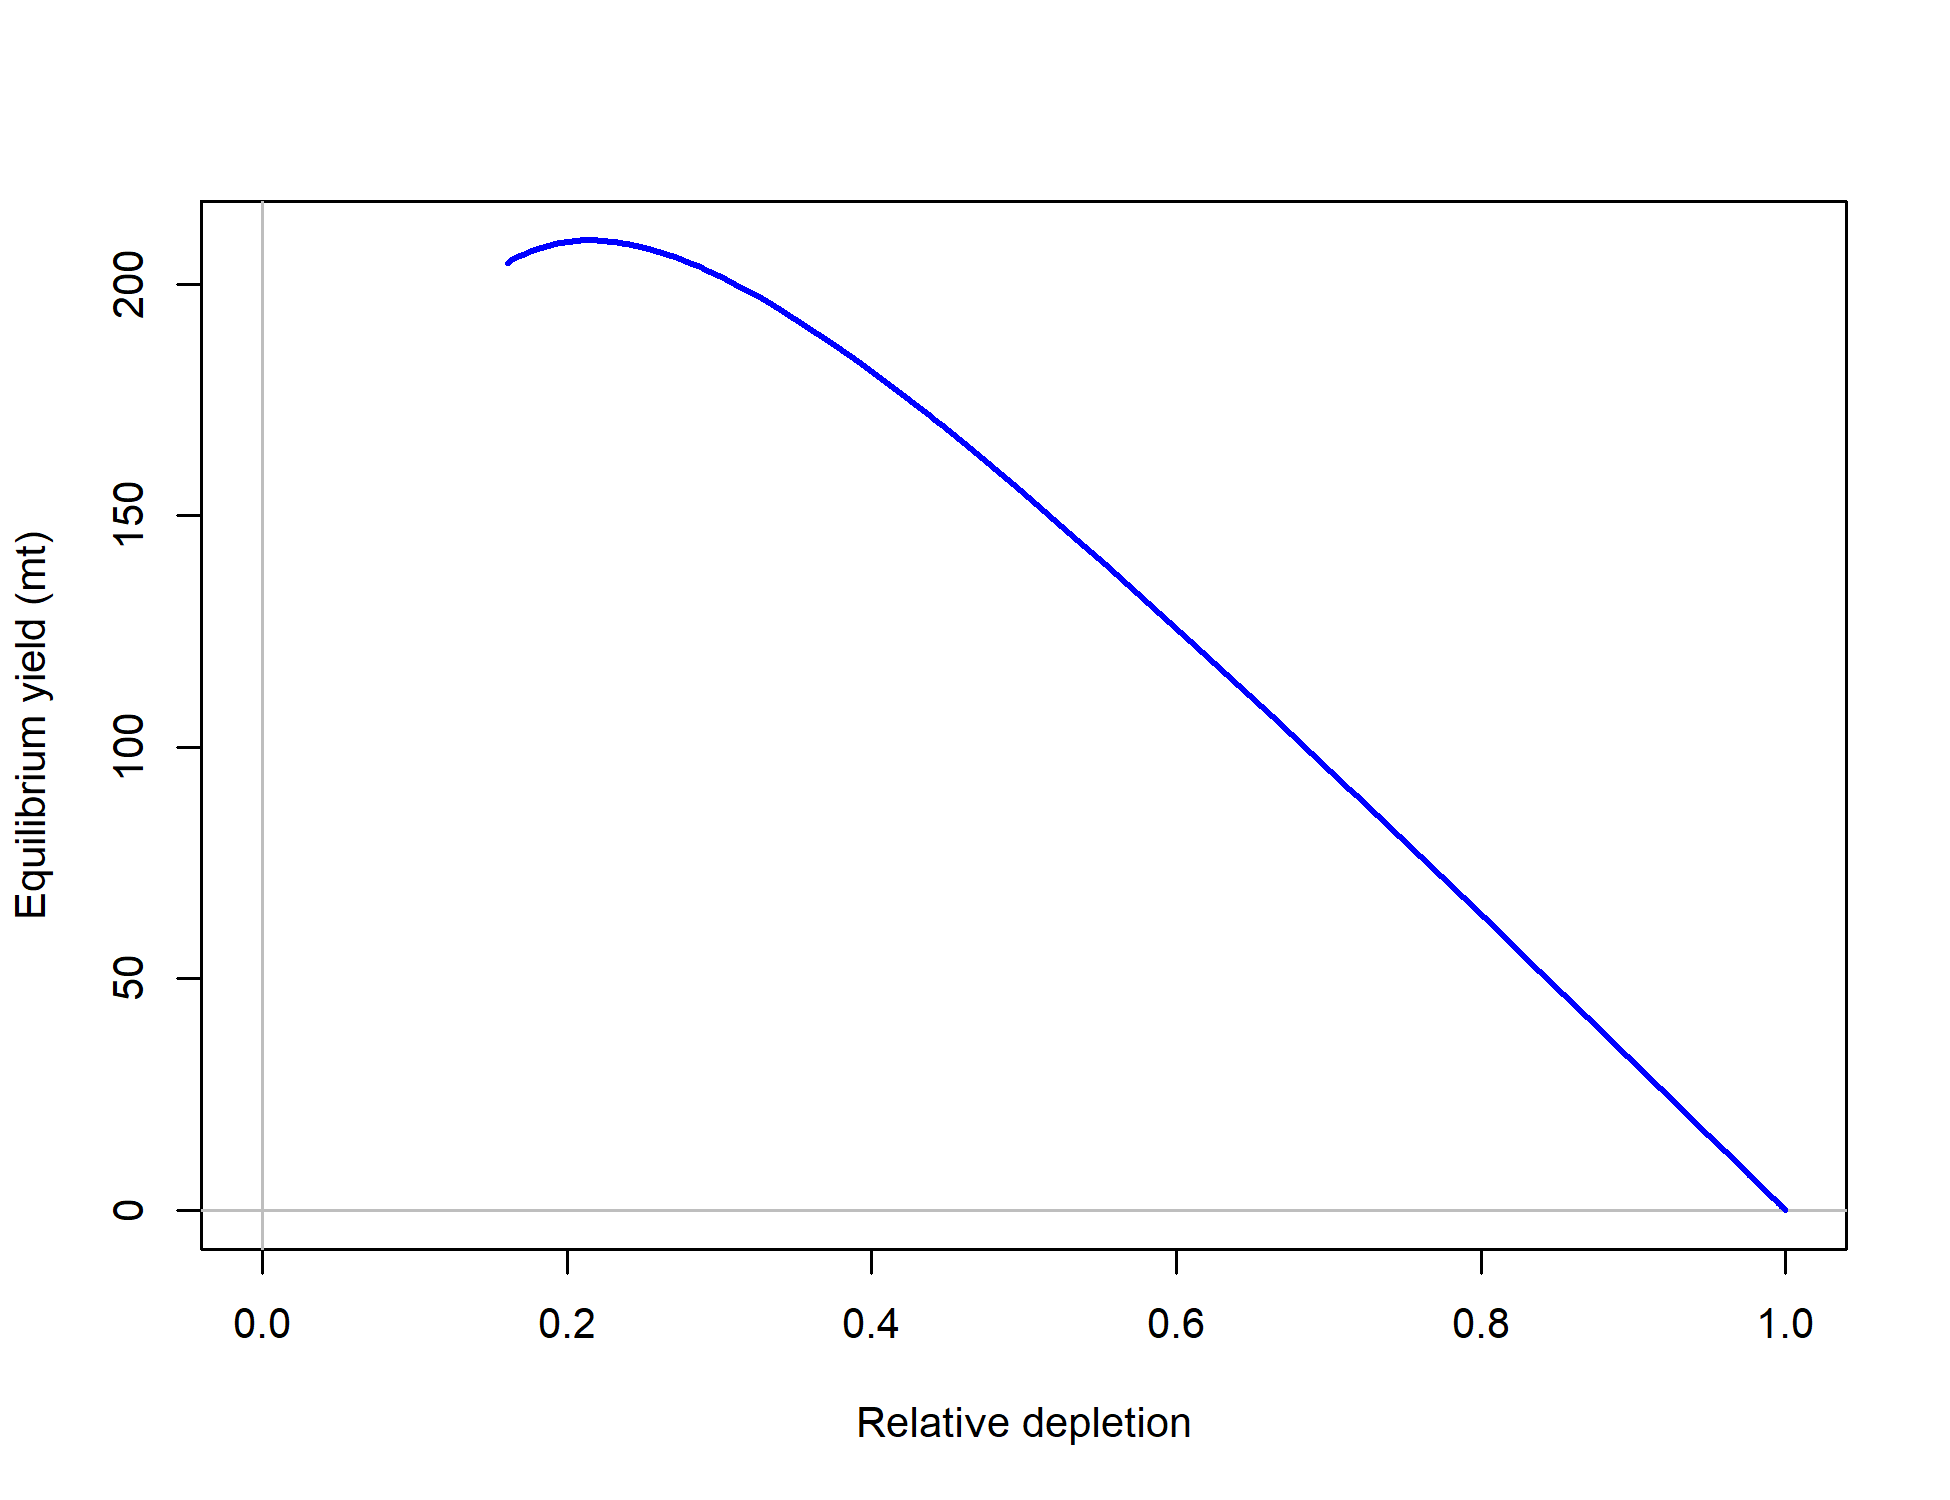
\includegraphics{r4ss/plots_mod1/yield1_yield_curve.png}
\caption{Equilibrium yield curve for the base case model. Values are
based on the 2018 fishery selectivity and with steepness fixed at 0.718.
\label{fig:Yield_all}}
\end{figure}

\FloatBarrier

\newpage

\subsection*{Research and Data Needs}\label{research-and-data-needs}
\addcontentsline{toc}{subsection}{Research and Data Needs}

We recommend the following research be conducted before the next
assessment:

\begin{enumerate}

\item \textbf{xxxx}: 

\item \textbf{xxxx}:

\item \textbf{xxxx}:

\item \textbf{xxxx}:

\item \textbf{xxxx}:

\end{enumerate}

\FloatBarrier

\newpage

\renewcommand{\thefigure}{\arabic{figure}}
\renewcommand{\thetable}{\arabic{table}}

\setcounter{figure}{0} \setcounter{table}{0}

\pagenumbering{arabic}

\section{Introduction}\label{introduction}

\subsection{Basic Information and Life
History}\label{basic-information-and-life-history}

\subsection{Early Life History}\label{early-life-history}

\subsection{Map}\label{map}

A map showing the scope of the assessment and depicting boundary at Pt.
Conception for the recreational fishing fleet (Figure
\ref{fig:assess_region_map}).

\subsection{Ecosystem Considerations}\label{ecosystem-considerations-1}

In this assessment, ecosystem considerations were not explicitly
included in the analysis. This is primarily due to a lack of relevant
data and results of analyses (conducted elsewhere) that could contribute
ecosystem-related quantitative information for the assessment.

\subsection{Fishery Information}\label{fishery-information}

\subsection{Summary of Management
History}\label{summary-of-management-history}

\subsection{Management Performance}\label{management-performance-1}

Table \ref{tab:mnmgt_perform}

\subsection{Fisheries Off Mexico or
Canada}\label{fisheries-off-mexico-or-canada}

\section{Assessment}\label{assessment}

\subsection{Data}\label{data}

Data used in the GBYR assessment are summarized in Figure
\ref{fig:data_plot}. Descriptions of the data sources are in the
following sections.

\subsubsection{Commercial Fishery
Landings}\label{commercial-fishery-landings}

\emph{Overview of gopher and black-and-yellow catch history}

Commercial fishery landings for gopher and black-and-yellow rockfishes
have not been reported consistently by species throughout the available
catch history (Figure \ref{fig:Catches_livedeadNS_gby}). The period from
1916-1935 indicates that only black-and-yellow rockfish were landed in
the commercial fishery, which then switched to predominately gopher
rockfish from 1937-1984. From 1985-1988 the landings data suggest that
only black-and-yellow rockfish were landed and not until 1995 are both
speices well-represented in the catches. There is not way to tease apart
the historical catches by species and even across north and south of Pt.
Conception prior to about 1995. This precludes the ability to model the
catch histories for eiether species accurately. Given these constraints,
all commercial dats were combined to represent one one commercial flee
in the assessment.

The stock assessment of gopher rockfish in 2005 did not include
black-and-yellow rockfish landings. A comparison of recreational and
commercial landings from the 2005 assessment to those used in this
assessment suggest the 2005 assessment may have included some
black-and-yellow rockfish landings (Figure
\ref{fig:Assessment_compare}). The 2005 assessment estimated
recreational landings from 1969-1980 based on a ratio of commercial to
recreational landings, where as this assessment makes use of the
California Catch Reconstruction landings estimates (Ralston et al.
\protect\hyperlink{ref-Ralston2010}{2010}).

\emph{Commercial Landings Data Sources}

Commercial landings in California are based on two primary data sources:
a cooperative port sampling program (California Cooperative Groundfish
Survey, \href{https://calcom.psmfc.org/}{CALCOM}) that collects
information including species composition data (i.e.~the proportion of
species landed in a sampling stratum), and landing receipts (sometimes
called ``fish tickets'') that are a record of pounds landed in a given
stratum. Strata in California are defined by market category, year,
quarter, gear group, port complex, and disposition (live or dead).
Although many market categories are named after actual species, catch in
a given market category can consist of several species. All landings
used in this assessment are ``expanded'' landings, i.e., species
composition data collected by port samplers were used to allocate pounds
recorded on landing receipts to species. Use of the ``Gopher Rockfish''
or the ``Black-and-Yellow Rockfish'' categories alone to represent
actual landings of GBY would not be accurate. See Pearson et al.
Appendix C (\protect\hyperlink{ref-Pearson2008}{2008}) for a simple
example of the expansion calculations. Data from the California
Cooperative Groundfish Survey, species compositions, and expanded
landings estimates are stored in the CALCOM database at the Pacific
States Marine Fisheries Commission, a central repository of commercial
landings data for the U.S. West Coast.

Commercial catches of black-and-yellow rockfish from 1916-1968 and for
gopher rockfish from 1937-1968 were queried (4 April 2019) from the
California Catch Reconstruction (Ralston et al.
\protect\hyperlink{ref-Ralston2010}{2010}). Landings in this database
are divided into trawl and `non-trawl.' Since the majority of GBYR are
caught in the commercial fixed gear fisheries, only estimated catch in
the `non-trawl' was used. A total of 0.154 mt (3.18\%) were removed from
Eureka commercial landings (based on current proportions of commercial
catch from north of Cape Mendocino in Eureka) since the assessment
represents the GBYR stock south of Cape Mendocino.

Commercial landings from 1969-2018 were queried for a final time from
the CALCOM database on 4 April 2019 (Table \ref{tab:commCatches}.
Commercial landings were also queried from PacFIN (Pacific Fisheries
Information Network) for a final time on 3 June 2019 for comparison to
CALCOM landings. There are very small differences in commercial landings
between CALCOM and PacFIN from 1981-2018 (Figure
\ref:fig:Calcom\_vs\_Pacfin\}). Landings estimates from CALCOM were used
in the assessment. Landings were stratified by year, quarter, live/dead,
market category, gear group, port complex, and source of species
composition data (actual port samples, borrowed samples, or assumed
nominal market category). Data from individual quarters were aggregated
at the year level. Fish landed live or dead were combined, due to
changes over time in the reliability of condition information (D.
Pearson, pers. comm.). From 1916-1968, on average, 74\% of GBYR were
landed north of Point Conception, which rose to 97\% from 1978-2018.
Given the smaller landings south of Point Conception and the similar
length composition of GBYR north and south of Pt. Conception, no spatial
separation was considered for the commercial fleet.

\subsubsection{Commercial Discards}\label{commercial-discards}

The West Coast Groundfish Observer Program (WCGOP) provides observer
data on discarding across fishery sectors back to 2003. Gopher and
black-and-yellow rockfishes have different depth-stratified commercial
fishery discard mortality rates (Pacific Fishery Managment Council
\protect\hyperlink{ref-PSMFC2018}{2018}). In consultation with WCGOP
staff, the STAT used estimates of total discard mortality from WCGOP's
Groundfish Expanded Mortality Multiyear (GEMM) report. WCGOP observes
between 1-5\% of nearshore fixed gear landings annually south of
\(40^\circ 10^\prime\) N. latitude (coverage rates available
\href{https://www.nwfsc.noaa.gov/research/divisions/fram/observation/data_products/sector_products.cfm\#ob}{here}).
The expanded estimates of total discard weight by species is calculated
as the ratio of the observed discard weight of the individual species
divided by the observed landed weight\\
from PacFIN landing receipts. WCGOP discard estimates for the nearshore
fixed gear fishery take into account the depth distribution of landings
in order to appropriately apply the depth-stratified discard mortality
rates by species (Somers, K.A., J. Jannot, V. Tuttle, K. Richerson and
McVeigh \protect\hyperlink{ref-Somers2018}{2018}). The discard mortality
for 2018 was estimated as an average of the discard mortality from
2013-2017. Discard mortality was estimated from the period prior to
WCGOP discard estimates (1916-2002) based on the average discard
mortality rate from 2003-2016 (2017 was excluded because 2017 discard
mortality was disproportionately higher than all other years) (Table
\ref{tab:CommCatches}).

\subsubsection{Commercial Fishery Length and Age
Data}\label{commercial-fishery-length-and-age-data}

Biological data from the commercial fisheries that caught GBYR were
extracted from CALCOM on 9 May 2019. The CALCOM length composition data
were catch-weighted to ``expanded'' length the raw lenght composition
data (Table \ref{tab:length_samples_fishery}). The 2005 assessment used
commercial length composition informtion from CALCOM, but did not
include black-and-yellow rockfish and is not directly comparable. The
2005 assessment used 2 cm length bins from 16-40 cm, where this
assessment uses 1 cm length bins from 4-40 cm. Sex was not available for
the majority (99.5\%) of the commercial length, and the assessment did
not find sexual dimorphism in growth for either species. We aggregated
the commercial length composition among all gears and regions south of
Cape Mendocino.

Discard length compositions from WCGOP (2003-2017) were expanded based
on the the discard estimates and were aggregated for all regions south
of Cape Mendocino and across all fixed gear fisheries.

A total of 46 ages were available for gopher rockfish from the
commercial fisheries 2009-2011, 2016, and 2018. Though sparse, the data
were included as conditional age-at-length for the commercial fleet.

The input sample sizes for commercial length composition data were
calculated via the Stewart Method for fisheries (Ian Stewart, personal
communication, IPHC):

\begin{centering}

Input effN = $N_{\text{trips}} + 0.138 * N_{\text{fish}}$ if $N_{\text{fish}}/N_{\text{trips}}$ is $<$ 44

Input effN = $7.06 * N_{\text{trips}}$ if $N_{\text{fish}}/N_{\text{trips}}$ is $\geq$ 44

\end{centering}

\subsubsection{Recreational Fishery Removals and
Discards}\label{recreational-fishery-removals-and-discards}

\emph{Historical recreational landings and discard, 1928-1980}

Ralston et al. (\protect\hyperlink{ref-Ralston2010}{2010}) reconstructed
estimates of recreational rockfish catch and discard in California,
1928-1980. Reported landings of total rockfish were allocated to species
based on several sources of species composition data. Estimates of GBYR
landings and discard (combined) from 1928-1979 are available from the
SWFSC. For this assessment, historical recreational catch was stratified
by year and area (north and south of Point Conception). The catches of
GBYR reported in Ralston et al.
(\protect\hyperlink{ref-Ralston2010}{2010}) are higher than expected
given the more recent catches of GBYR south of Pt. Conception and the
species' ranges (Figure \ref{fig:Catches_original}). The California
Catch Reconstruction used a linear ramp from from 1928-1936 that was not
altered in this assessment. From 1937-1979 linear ramp to the average
recreational landing from 1980 and 1983 (1981-1982 catches interpolated
as described in the next section) of 4.3 mt. The recreational catches
north of Pt. Conception were not altered from the original catch
reconstruction. The resulting alternate recreational catch streams are
in (Table \ref{tab:Rec_removal} and Figure \ref{fig:Catches_alternate}).

\emph{Marine Recreational Fisheries Statistics Survey (MRFSS),
1980-2003}

From 1980-2003, the Marine Recreational Fisheries Statistics Survey
(MRFSS) executed a dockside (angler intercept) sampling program in
Washington, Oregon, and California. Data from this survey are available
from the Recreational Fisheries Information Network
\href{www.recfin.org}{RecFIN}. RecFIN serves as a repository for
recreational fishery data for California, Oregon, and Washington. Catch
estimates for years 1980-2003 were downloaded on 23 March 2019 (), and
are consistent with the previous assessment {[}Key2005{]}. - need to
check again)

MRFSS-era recreational removals for California were estimated for two
regions: north and south of Point Conception. No finer-scale estimates
of landings are available for this period. Catches were downloaded in
numbers and weight. Catch in weight is sometimes missing from the
database due to missing average weight estimates. We estimated average
weights based on adjacent strata as needed, although the effect was
relatively minor (7.4 mt over all years for gopher rockfish and 0.6 mt
for black-and-yellow rockfish). Data were not available for the CPFVs in
Northern California from 1980-1982, and we used the average value from
this mode and region from 1983-1987 for these three years. MRFSS
sampling was temporarily suspended from 1990-1992, and we used linear
interpolation to fill the missing years. Sampling of CPFVs in Northern
California was further delayed, and the linear interpolation spans the
period 1990-1995 for this boat mode and region. Landings data for the
shore-based modes (beach/bank, man-made/jetty and shore) were sparse
throughout the MRFSS sampling. All three shore-based modes were combined
by region and linear interpolations were applied missing data in 1981
for the Northern California and 1995, 1996-2001, and 2004 in Southern
California.

Catches from north of Cape Mendocino were removed based on a CRFS-era
average of fraction of recreational landings north of Cape Mendocino by
mode (3.3\% of shore-based, 0.1\% of CPFV, and 0.2\% of private/rental
were removed). From 1980-1989, San Luis Obispo County was sampled as
part of Southern California (personal observation from MRFSS Type 3
sampler examined catch where county is available for 1980-2004). This
assessment separates the recreational fleet at Pt. Conception.
Recreational landings were re-allocated from southern California from
1980-1992 by fleet based on the average proportion of recreational
landings in northern California from 1996-2004 (after sampling of the
CPFV fleet in northern California resumed). The average proportion
re-allocated from southern to northern California for the CPFV mode was
85\%, 97\% for the private/rental mode, and 81\% for the shore-based
modes. Data were pooled over all years and modes to estimate the
landings re-allocation for the shore-based modes. Total recreational
landings for 1981 and 1982 were 18.8 mt and 18.6 mt, respectively. These
landings were \textgreater{}60 mt lower than any of the neighboring
years. Landings from 1981-1982 were interpolated from the 1980 and 1983
landings.

\emph{California Recreational Fisheries Survey (CRFS), 2004-2016}

MRFSS was replaced with the California Recreational Fisheries Survey
(CRFS) beginning January 1, 2004. Among other improvements to MRFSS,
CRFS provides higher sampling intensity, finer spatial resolution (6
districts vs.~2 regions), and onboard CPFV sampling. Estimates of catch
from 2004-2018 were downloaded from the RecFIN database a final time on
4 June 2019, We queried and aggregated CRFS data to match the structure
of the MRFSS data, by year, and region (Table \ref{tab:Rec_removal}.
Catches in the shore-based modes are small compared to the CPFV and
private rental modes. All modes are combined, but separated at Point
Conception for two recreational fleets in this assessment, just as was
done for the California Catch Recontruction and MRFSS time series.

\emph{Recreational Discard}

Recreational discards were only added to the California Catch
Reconstruction landings, as Ralston et al.
(\protect\hyperlink{ref-Ralston2010}{2010}) did not address discards for
the recreational recontruction. Recreational removals from the
California Department of Fish and Wildlife MRFSS era (1980-2003)
includes catch type A + B1. Catch type A refers to estimates of catch
based on sampler-examined catch. Catch type B1 includes mainly
angler-reported discard, but also angler-reported retained fish that
were unavailable to the sampler during the interview (e.g., fillets).
(2004-2018) databases. The CRFS era removals account for
depth-stratified discard mortality rate and the catch time series
includes both retained and discarded catch (toal mortality). We
calculated the ratio of dead discards to total mortality from the CRFS
era by region and mode. The region average across modes was applied to
the California Catch Reconstruction as a constant. The result added
4.68\% annually to recreational removals north of Pt. Conception and
4.05\% annutally to the removals South of Pt. Conception). The final
time series of landings and discard mortality are in Table
\ref{tab:Rec_removal}.

\subsubsection{Recreational Fishery Length and Age
Data}\label{recreational-fishery-length-and-age-data}

Recreational length composition samples for California were obtained
from several sources, depending on the time period and boat mode (Table
\ref{tab:length_samples_fishery}). This assessment makes use of a much
longer time series of length composition data, relative to the previous
assessment, as described below. Input sample sizes for recreational
length composition data were based on the number of observed trips, when
available. Other proxies that were used to estimate the number of trips
are described below.

There were no standardized coastwide surveys measure retained or
discarded fish from the recreational fleet prior to 1980.

\emph{CPFV length composition data, 1959-1978}

The earliest available length data for this assessment were described by
Karpov et al. (\protect\hyperlink{ref-Karpov1995}{1995}), who assembled
a time series (1959-1972) of available California CPFV length data (made
available courtesy of W. Van Buskirk). For GBYR, data from 1959-1961 and
1966 were available north of Pt. Conception and from 1959-1961 from
south of Pt Conception. A total of 716 (680 north of Pt. Conception)
unsexed measurement of retained fish (no discards, ) were included in
the assessment (Table ). Sampling of these length data did not follow
consistent protocol over time and areas (data are unweighted), and
therefore may not be representative of total catch. Since the number of
trips sampled was not reported by Karpov et al. (1995), we assume the
number of sampled trips is proportional to the number of measured fish
in each year, and estimated the number of trips using the ratio of fish
measured per trip in the MRFSS data (roughly 10 fish per trip).

Collins and Crooke (n.d.) conducted an onboard observer survey of the
CPFV fleet in southern California from 1975-1978. A total of 1,308 GBYR
lengths were available from the study and were assumed to all be from
retained fish. Ally et al. (\protect\hyperlink{ref-Ally1991}{1991})
conducted an onboard observer program of thee CPFV fleet from 1985-1987
in southern California. Becuase MRFSS data were available for this time
period as well and represents multiple recreational modes, the Ally et
al. (\protect\hyperlink{ref-Ally1991}{1991}) length data were not used
in the assessment.

\emph{MRFSS Recreational Length Data, 1980-1989 and 1993-2003}

Unsexed length data of retained fish were collected by MRFSS dockside
samplers and downloaded from the RecFIN website. We identified a subset
of lengths that were converted from weight measurements, and these were
excluded from the final data set (Table
\ref{tab:length_sample_fishery}). The length measurements from Collins
and Crooke (n.d.) from 1975-1978 are assumed to all be from retained
fish. As of 2003, the CDFW Onboard Observer program has taken length
measurements for discarded fish. The retained catch is measured during
the dockside (angler intercept) surveys.

The number of trips used as initial sample sizes for the MRFSS was based
on\ldots{}.

During the recent restructiong of the CRFS data on RecFIN, a ``trip''
identifier was not carried over for all modes, and trip-level sample
sizes could not be extracted from the biological detail table on RecFIN.
A proxy for initial sample sizes for 2004-2018 were developed using the
2015 data for which I had access to raw data files by mode from CDFW.\\
In more recent years, sampling of the shore-based modes has declined and
were not sampled at all in 2018. Samples sizes were calculated by mode
as the number of port-days (or site-days for shore-based modes) during
bi-weekly intervals (e.g., Jan 1-15, Jan 16-31, etc). The number of
port-days sampled in the bi-weekly intervals was used as the initial
sample size for number of trips to calculate initial input sample sizes
using Ian Stewart's method (described above). All lenght data were
re-weighted in the assessment model.

\subsubsection{Fishery-Dependent Indices of
Abundance}\label{fishery-dependent-indices-of-abundance}

\textbf{Data Source 1}

\emph{Data Source 1 Index Standardization}

Table \ref{tab:Indices})

(Table \ref{'tab:length_samples_survey}) \emph{Data Source 1 Length
Composition}

\textbf{Data Source 2}

\textbf{Data Source 3}

\subsubsection{Fishery-Independent Data
Sources}\label{fishery-independent-data-sources}

\textbf{Data Source 1}

\emph{Data Source 1 Index Standardization}

\emph{Data Source 1 Length Composition}

\textbf{Data Source 2}

\subsubsection{Biological Parameters and
Data}\label{biological-parameters-and-data}

\textbf{Length and Age Compositions}

Length compositions were provided from the following sources:

\begin{itemize}[noitemsep,nolistsep,topsep=0pt]
  \item Source 1 (\emph{type, e.g., commercial dead fish, research, recreational}, yyyy-yyyy)    
  \item Source 2 (\emph{type}, yyyy-yyyy)    
  \item Source 3 (\emph{research}, yyyy, yyyy, yyyy, yyyy) 
\end{itemize}

The length composition of all fisheries aggregated across time by fleet
is in Figure \ref{fig:comp_lendat_aggregated_across_time}. Descriptions
and details of the length composition data are in the above section for
each fleet or survey.

\vspace{.5cm} \textbf{Age Structures}

von Bertalanffy growth curve (Bertalanffy
\protect\hyperlink{ref-vonB1938}{1938}),
\(L_i = L_{\infty}e^{(-k[t-t_0])}\), where \(L_i\) is the length (cm) at
age \(i\), \(t\) is age in years, \(k\) is rate of increase in growth,
\(t_0\) is the intercept, and \(L_{\infty}\) is the asymptotic length.

\vspace{.5cm} \textbf{Aging Precision and Bias}

\vspace{.5cm} \textbf{Weight-Length}

\vspace{.5cm} \textbf{Sex Ratio, Maturity, and Fecundity}

\vspace{.5cm} \textbf{Natural Mortality}

\vspace{.5cm}

\subsubsection{Environmental or Ecosystem Data Included in the
Assessment}\label{environmental-or-ecosystem-data-included-in-the-assessment}

In this assessment, neither environmental nor ecosystem considerations
were explicitly included in the analysis. This is primarily due to a
lack of relevant data and results of analyses (conducted elsewhere) that
could contribute ecosystem-related quantitative information for the
assessment.

\subsection{Previous Assessments}\label{previous-assessments}

\subsubsection{History of Modeling Approaches Used for this
Stock}\label{history-of-modeling-approaches-used-for-this-stock}

\subsubsection{yyyy Assessment
Recommendations}\label{yyyy-assessment-recommendations}

\begin{description}[style=unboxed]

  \item[Recommendation 1: ] \hfill \\

   STAT response: xxxxx

\item[Recommendation 2: ] \hfill \\

  STAT response: xxxxx

\item[Recommendation 3: ] \hfill \\

  STAT response: xxxx

  
\end{description}

\subsection{Model Description}\label{model-description}

\subsubsection{Transition to the Current Stock
Assessment}\label{transition-to-the-current-stock-assessment}

\subsubsection{Summary of Data for Fleets and
Areas}\label{summary-of-data-for-fleets-and-areas}

There are xxx fleets in the base model. They include:

\emph{Commercial}: The commercial fleets include \ldots{}

\emph{Recreational}: The recreational fleets include \ldots{}

\emph{Research}: There are xx sources of fishery-independent data
available \ldots{}

\subsubsection{Other Specifications}\label{other-specifications}

\subsubsection{Modeling Software}\label{modeling-software}

The STAT team used Stock Synthesis 3 version 3.30.05.03 by Dr.~Richard
Methot at the NWFSC. This most recent version was used, since it
included improvements and corrections to older versions. The r4SS
package (GitHub release number v1.27.0) was used to post-processing
output data from Stock Synthesis.

\subsubsection{Data Weighting}\label{data-weighting}

\subsubsection{Priors}\label{priors}

The log-normal prior for female natural mortality were based on a
meta-analysis completed by Hamel
(\protect\hyperlink{ref-Hamel2015}{2015}), as described under ``Natural
Mortality.'' Female natural mortality was fixed at the median of the
prior, 0.xxx for an assumed maximum age of xx. An uninformative prior
was used for the male offset natural mortality, which was estimated.

The prior for steepness (\emph{h}) assumes a beta distribution with
parameters based on an update for the Thorson-Dorn rockfish prior (Dorn,
M. and Thorson, J., pers. comm.), which was endorsed by the Science and
Statistical Committee in 2018. The prior is a beta distribution with
\(mu\)=0.xxx and \(sigma\)=0.xxx. Steepness is fixed in the base model
at the mean of the prior. The priors were applied in sensitivity
analyses where these parameters were estimated.

\subsubsection{Estimated and Fixed
Parameters}\label{estimated-and-fixed-parameters}

A full list of all estimated and fixed parameters is provided in Tables
\ref{tab:model_params}.

The base model has a total of xxx estimated parameters in the following
categories:

\begin{itemize}
  \item xxx,
  \item xxx
  \item xxx, and
  \item xxx selectivity parameters
\end{itemize}

The estimated parameters are described in greater detail below and a
full list of all estimated and parameters is provided in Table
\ref{tab:model_params}.

\emph{Growth.}

\emph{Natural Mortality.}

\emph{Selectivity.}

\emph{Other Estimated Parameters.}

\emph{Other Fixed Parameters.}

\subsection{Model Selection and
Evaluation}\label{model-selection-and-evaluation}

\subsubsection{Key Assumptions and Structural
Choices}\label{key-assumptions-and-structural-choices}

\subsubsection{Alternate Models
Considered}\label{alternate-models-considered}

\subsubsection{Convergence}\label{convergence}

\subsection{Response to the Current STAR Panel
Requests}\label{response-to-the-current-star-panel-requests}

\begin{description}[style=sameline]

\item[Request No. 1: ] \hfill \\
  
\textbf{Rationale:} xxx   
    
\textbf{STAT Response:} xxx


\item[Request No. 2: ] \hfill \\


\textbf{Rationale:} xxx 


\textbf{STAT Response:} xxx
    

\item[Request No. 3: ] \hfill \\

\textbf{Rationale:} x.  
    
  
\textbf{STAT Response:} xxx

\item[Request No. 4: ] \hfill \\

\textbf{Rationale:} xxx 
    
    
\textbf{STAT Response:} xxx


\item[Request No. 5: ] \hfill \\

\textbf{Rationale:} xxx
  
\textbf{STAT Response:} xxx  
    


\end{description}

\subsection{Base Case Model Results}\label{base-case-model-results}

The following description of the model results reflects a base model
that incorporates all of the changes made during the STAR panel (see
previous section). The base model parameter estimates and their
approximate asymptotic standard errors are shown in Table
\ref{tab:model_params} and the likelihood components are in Table
\ref{tab:like_components}. Estimates of derived reference points and
approximate 95\% asymptotic confidence intervals are shown in Table
\ref{tab:Ref_pts_mod1}. Time-series of estimated stock size over time
are shown in Table \ref{tab:Timeseries_mod1}.

\subsubsection{Parameter Estimates}\label{parameter-estimates}

The additional survey variability (process error added directly to each
year's input variability) for all surveys was estimated within the
model.

(Figure
\ref{fig:ts11_Age-0_recruits_(1000s)_with_95_asymptotic_intervals} ).

The stock-recruit curve \ldots{} Figure \ref{fig:SR_curve2} with
estimated recruitments also shown.

\subsubsection{Fits to the Data}\label{fits-to-the-data}

Model fits to the indices of abundance, fishery length composition,
survey length composition, and conditional age-at-length observations
are all discussed below.

\subsubsection{Uncertainty and Sensitivity
Analyses}\label{uncertainty-and-sensitivity-analyses}

A number of sensitivity analyses were conducted, including:

\begin{enumerate}

  \item Sensitivity 1
  
  \item Sensitivity 2
  
  \item Sensitivity 3
  
  \item Sensitivity 4
  
  \item Sensitivity 5, etc/
  
  
\end{enumerate}

\subsubsection{Retrospective Analysis}\label{retrospective-analysis}

\subsubsection{Likelihood Profiles}\label{likelihood-profiles}

\subsubsection{Reference Points}\label{reference-points-1}

Reference points were calculated using the estimated selectivities and
catch distribution among fleets in the most recent year of the model,
(2017). Sustainable total yield (landings plus discards) were 169 mt
when using an \(SPR_{50\%}\) reference harvest rate and with a 95\%
confidence interval of 104 mt based on estimates of uncertainty. The
spawning biomass equivalent to 40\% of the unfished level
(\(SB_{40\%}\)) was 554 mt.

(Figure
\ref{fig:ts7_Spawning_biomass_(mt)_with_95_asymptotic_intervals_intervals}

The 2018 spawning biomass relative to unfished equilibrium spawning
biomass is above/below the target of 40\% of unfished levels (Figure
\ref{fig:ts9_Spawning_depletion_with_95_asymptotic_intervals_intervals}).
The relative fishing intensity, \((1-SPR)/(1-SPR_{50\%})\), has been xxx
the management target for the entire time series of the model.

Table \ref{tab:Ref_pts_mod1} shows the full suite of estimated reference
points for the base model and Figure \ref{fig:yield1_yield_curve} shows
the equilibrium curve based on a steepness value xxx.

\section{Harvest Projections and Decision
Tables}\label{harvest-projections-and-decision-tables}

The forecasts of stock abundance and yield were developed using the
final base model, with the forecasted projections of the OFL presented
in Table \ref{tab:OFL_projection}.

The forecasted projections of the OFL for each model are presented in
Table \ref{tab:Decision_table_mod1}.

\section{Regional Management
Considerations}\label{regional-management-considerations}

\section{Research Needs}\label{research-needs}

There are a number of areas of research that could improve the stock
assessment for GBYR. Below are issues identified by the STAT team and
the STAR panel:

\begin{enumerate}

\item \textbf{xxxx}: 

\item \textbf{xxxx}:

\item \textbf{xxxx}:

\item \textbf{xxxx}:

\item \textbf{xxxx}:

\end{enumerate}

\section{Acknowledgments}\label{acknowledgments}

\newpage

\FloatBarrier

\section{Tables}\label{tables}

\FloatBarrier

\begin{longtable}{c>{\centering}p{1in}>{\centering}p{.6in}>{\centering}p{1in}l}
\caption{Commercial landings and discards (mt) from the commercial 
                                fisheries. Data sources are the California Catch 
                                Reconstruction, CALCOM, and WCGOP GEMM report.} \\ 
  \hline
Year & Landings & Discards & Total Commercial Removals & Source \\ 
  \hline  \endfirsthead \caption[]{Commercial landings and discards (mt) from the commercial 
                                fisheries. Data sources are the California Catch 
                                Reconstruction, CALCOM, and WCGOP GEMM report.} \label{tab:CommCatches} \\ \hline Year & Landings & Discards & Total Commercial Removals & Source \\ \hline  \endhead \hline \multicolumn{4}{l}{\textit{Continues next page}} \ 
                                 \endfoot
                                 \endlastfoot \hline
1916 & 3.88 & 0.38 & 4.27 & Catch Reconstruction \\ 
  1917 & 6.03 & 0.59 & 6.63 & Catch Reconstruction \\ 
  1918 & 7.06 & 0.69 & 7.75 & Catch Reconstruction \\ 
  1919 & 4.91 & 0.48 & 5.39 & Catch Reconstruction \\ 
  1920 & 5.01 & 0.49 & 5.50 & Catch Reconstruction \\ 
  1921 & 4.13 & 0.41 & 4.54 & Catch Reconstruction \\ 
  1922 & 3.56 & 0.35 & 3.90 & Catch Reconstruction \\ 
  1923 & 3.84 & 0.38 & 4.22 & Catch Reconstruction \\ 
  1924 & 2.22 & 0.22 & 2.44 & Catch Reconstruction \\ 
  1925 & 2.78 & 0.27 & 3.05 & Catch Reconstruction \\ 
  1926 & 4.48 & 0.44 & 4.92 & Catch Reconstruction \\ 
  1927 & 3.81 & 0.37 & 4.18 & Catch Reconstruction \\ 
  1928 & 4.60 & 0.45 & 5.06 & Catch Reconstruction \\ 
  1929 & 3.81 & 0.37 & 4.18 & Catch Reconstruction \\ 
  1930 & 5.40 & 0.53 & 5.93 & Catch Reconstruction \\ 
  1931 & 1.93 & 0.19 & 2.11 & Catch Reconstruction \\ 
  1932 & 6.24 & 0.61 & 6.85 & Catch Reconstruction \\ 
  1933 & 2.58 & 0.25 & 2.84 & Catch Reconstruction \\ 
  1934 & 1.75 & 0.17 & 1.92 & Catch Reconstruction \\ 
  1935 & 0.43 & 0.04 & 0.47 & Catch Reconstruction \\ 
  1936 & 0.01 & 0.00 & 0.01 & Catch Reconstruction \\ 
  1937 & 7.27 & 0.71 & 7.98 & Catch Reconstruction \\ 
  1938 & 10.29 & 1.01 & 11.30 & Catch Reconstruction \\ 
  1939 & 13.13 & 1.29 & 14.42 & Catch Reconstruction \\ 
  1940 & 16.90 & 1.66 & 18.56 & Catch Reconstruction \\ 
  1941 & 17.06 & 1.67 & 18.73 & Catch Reconstruction \\ 
  1942 & 8.55 & 0.84 & 9.38 & Catch Reconstruction \\ 
  1943 & 11.00 & 1.08 & 12.08 & Catch Reconstruction \\ 
  1944 & 0.05 & 0.00 & 0.05 & Catch Reconstruction \\ 
  1945 & 0.59 & 0.06 & 0.65 & Catch Reconstruction \\ 
  1946 & 16.71 & 1.64 & 18.35 & Catch Reconstruction \\ 
  1947 & 26.71 & 2.62 & 29.33 & Catch Reconstruction \\ 
  1948 & 23.95 & 2.35 & 26.30 & Catch Reconstruction \\ 
  1949 & 18.29 & 1.79 & 20.09 & Catch Reconstruction \\ 
  1950 & 17.15 & 1.68 & 18.83 & Catch Reconstruction \\ 
  1951 & 24.83 & 2.44 & 27.26 & Catch Reconstruction \\ 
  1952 & 27.59 & 2.71 & 30.29 & Catch Reconstruction \\ 
  1953 & 32.30 & 3.17 & 35.47 & Catch Reconstruction \\ 
  1954 & 40.75 & 4.00 & 44.74 & Catch Reconstruction \\ 
  1955 & 29.49 & 2.89 & 32.38 & Catch Reconstruction \\ 
  1956 & 40.66 & 3.99 & 44.65 & Catch Reconstruction \\ 
  1957 & 37.52 & 3.68 & 41.20 & Catch Reconstruction \\ 
  1958 & 33.56 & 3.29 & 36.86 & Catch Reconstruction \\ 
  1959 & 19.62 & 1.92 & 21.54 & Catch Reconstruction \\ 
  1960 & 11.30 & 1.11 & 12.41 & Catch Reconstruction \\ 
  1961 & 17.49 & 1.72 & 19.20 & Catch Reconstruction \\ 
  1962 & 27.18 & 2.67 & 29.85 & Catch Reconstruction \\ 
  1963 & 22.29 & 2.19 & 24.48 & Catch Reconstruction \\ 
  1964 & 16.55 & 1.62 & 18.17 & Catch Reconstruction \\ 
  1965 & 21.50 & 2.11 & 23.61 & Catch Reconstruction \\ 
  1966 & 13.44 & 1.32 & 14.76 & Catch Reconstruction \\ 
  1967 & 6.70 & 0.66 & 7.36 & Catch Reconstruction \\ 
  1968 & 8.29 & 0.81 & 9.10 & Catch Reconstruction \\ 
  1969 & 9.99 & 0.98 & 10.97 & CALCOM \\ 
  1970 & 14.21 & 1.39 & 15.60 & CALCOM \\ 
  1971 & 14.41 & 1.41 & 15.83 & CALCOM \\ 
  1972 & 19.42 & 1.91 & 21.33 & CALCOM \\ 
  1973 & 31.43 & 3.08 & 34.51 & CALCOM \\ 
  1974 & 33.41 & 3.28 & 36.69 & CALCOM \\ 
  1975 & 33.08 & 3.25 & 36.33 & CALCOM \\ 
  1976 & 33.90 & 3.33 & 37.23 & CALCOM \\ 
  1977 & 30.13 & 2.96 & 33.09 & CALCOM \\ 
  1978 & 43.41 & 4.26 & 47.67 & CALCOM \\ 
  1979 & 34.24 & 3.36 & 37.60 & CALCOM \\ 
  1980 & 63.65 & 6.24 & 69.89 & CALCOM \\ 
  1981 & 52.67 & 5.17 & 57.84 & CALCOM \\ 
  1982 & 38.96 & 3.82 & 42.78 & CALCOM \\ 
  1983 & 26.89 & 2.64 & 29.52 & CALCOM \\ 
  1984 & 14.82 & 1.45 & 16.27 & CALCOM \\ 
  1985 & 8.42 & 0.83 & 9.25 & CALCOM \\ 
  1986 & 25.49 & 2.50 & 27.99 & CALCOM \\ 
  1987 & 34.21 & 3.36 & 37.57 & CALCOM \\ 
  1988 & 55.73 & 5.47 & 61.20 & CALCOM \\ 
  1989 & 45.48 & 4.46 & 49.94 & CALCOM \\ 
  1990 & 46.77 & 4.59 & 51.36 & CALCOM \\ 
  1991 & 68.85 & 6.75 & 75.60 & CALCOM \\ 
  1992 & 83.99 & 8.24 & 92.23 & CALCOM \\ 
  1993 & 74.09 & 7.27 & 81.35 & CALCOM \\ 
  1994 & 60.06 & 5.89 & 65.95 & CALCOM \\ 
  1995 & 91.42 & 8.97 & 100.39 & CALCOM \\ 
  1996 & 94.71 & 9.29 & 104.00 & CALCOM \\ 
  1997 & 69.37 & 6.81 & 76.18 & CALCOM \\ 
  1998 & 65.28 & 6.40 & 71.68 & CALCOM \\ 
  1999 & 62.70 & 6.15 & 68.85 & CALCOM \\ 
  2000 & 53.91 & 5.29 & 59.20 & CALCOM \\ 
  2001 & 53.41 & 5.24 & 58.65 & CALCOM \\ 
  2002 & 42.28 & 4.15 & 46.42 & CALCOM \\ 
  2003 & 20.18 & 13.04 & 33.22 & CALCOM \& WCGOP \\ 
  2004 & 26.27 & 2.66 & 28.93 & CALCOM \& WCGOP \\ 
  2005 & 28.09 & 3.33 & 31.42 & CALCOM \& WCGOP \\ 
  2006 & 23.87 & 4.10 & 27.96 & CALCOM \& WCGOP \\ 
  2007 & 30.14 & 4.50 & 34.64 & CALCOM \& WCGOP \\ 
  2008 & 36.06 & 1.63 & 37.69 & CALCOM \& WCGOP \\ 
  2009 & 35.42 & 5.38 & 40.80 & CALCOM \& WCGOP \\ 
  2010 & 38.65 & 3.92 & 42.57 & CALCOM \& WCGOP \\ 
  2011 & 42.28 & 5.72 & 48.01 & CALCOM \& WCGOP \\ 
  2012 & 33.46 & 1.93 & 35.39 & CALCOM \& WCGOP \\ 
  2013 & 33.17 & 2.85 & 36.02 & CALCOM \& WCGOP \\ 
  2014 & 36.15 & 2.85 & 39.00 & CALCOM \& WCGOP \\ 
  2015 & 43.18 & 2.93 & 46.11 & CALCOM \& WCGOP \\ 
  2016 & 36.84 & 2.42 & 39.26 & CALCOM \& WCGOP \\ 
  2017 & 41.51 & 1.65 & 43.15 & CALCOM \& WCGOP \\ 
  2018 & 46.08 & 2.54 & 48.62 & CALCOM \& WCGOP \\ 
   \hline
\hline
\end{longtable}

\FloatBarrier

\begin{table}[ht]
\centering
\caption{Length composition sample sizes for fishery dependent data. Continuous years begin in 1975. 
           Recreational north samples include Karpov et al., MRFSS, and CRFS data. 
           Recreational south samples include Karpov et al., Collins and Crooke unpub.,
           Ally et al. 1991, MRFSS, and CRFS data.} 
\label{tab:length_samples_fishery}
\scalebox{0.76}{
\begin{tabular}{l>{\centering}p{0.6in}>{\centering}p{0.6in}>{\centering}p{0.6in}>{\centering}p{0.6in}>{\centering}p{0.6in}>{\centering}p{0.6in}>{\centering}p{0.6in}>{\centering}p{0.6in}>{\centering}p{0.6in}>{\centering}p{0.6in}}
  \hline
   \multicolumn{1}{c}{} & \multicolumn{2}{c}{CALCOM} & \multicolumn{2}{c}{WCGOP} & \multicolumn{2}{c}{Rec North} & \multicolumn{2}{c}{Rec South} & \multicolumn{2}{c}{Deb VW} \\  \cmidrule(lr){2-3} \cmidrule(lr){4-5} \cmidrule(lr){6-7} \cmidrule(lr){8-9} \cmidrule(lr){10-11}
  Year & Trips & Lengths & Trips & Lengths & Trips & Lengths & Trips & Lengths & Trips & Lengths \\ 
  \hline
1959 &  &  &  &  &  27 & 271 & 2.10 &  21 &  &  \\ 
  1960 &  &  &  &  &  39 & 394 & 1.40 &  14 &  &  \\ 
  1961 &  &  &  &  &   1 &   8 & 0.10 &   1 &  &  \\ 
  1966 &  &  &  &  &   1 &   7 &  &  &  &  \\ 
  1975 &  &  &  &  &  &  & 50.00 & 159 &  &  \\ 
  1976 &  &  &  &  &  &  & 73.00 & 224 &  &  \\ 
  1977 &  &  &  &  &  &  & 96.00 & 392 &  &  \\ 
  1978 &  &  &  &  &  &  & 91.00 & 533 &  &  \\ 
  1979 &  &  &  &  &  &  &  &  &  &  \\ 
  1980 &  &  &  &  &   4 & 164 & 21.00 &  53 &  &  \\ 
  1981 &  &  &  &  &   1 &  19 & 30.00 & 100 &  &  \\ 
  1982 &  &  &  &  &   1 &  50 & 17.00 &  58 &  &  \\ 
  1983 &  &  &  &  &   6 & 323 & 60.00 & 170 &  &  \\ 
  1984 &  &  &  &  &  14 & 849 & 42.00 & 150 &  &  \\ 
  1985 &  &  &  &  &  35 & 1027 & 34.00 & 180 &  &  \\ 
  1986 &  &  &  &  &  36 & 826 & 28.00 &  86 &  &  \\ 
  1987 &   2 &  82 &  &  &  28 & 392 & 5.00 &   7 &  14 &  73 \\ 
  1988 &  &  &  &  &  30 & 303 & 10.00 &  30 &  54 & 664 \\ 
  1989 &  &  &  &  &  19 & 303 & 7.00 &  11 &  70 & 727 \\ 
  1990 &  &  &  &  &  &  &  &  &  17 & 109 \\ 
  1991 &  &  &  &  &  &  &  &  &  38 & 722 \\ 
  1992 &  56 & 671 &  &  &  &  &  &  &  55 & 838 \\ 
  1993 & 148 & 1648 &  &  &  14 & 1094 & 8.00 &  24 &  75 & 614 \\ 
  1994 & 170 & 1379 &  &  &  12 & 608 & 1.00 &  15 &  86 & 735 \\ 
  1995 & 174 & 1523 &  &  &  &  &  &  &  90 & 1171 \\ 
  1996 & 256 & 3270 &  &  &  74 & 607 & 14.00 &  32 & 100 & 1364 \\ 
  1997 & 140 & 1319 &  &  &  95 & 1424 & 7.00 &  23 & 107 & 1415 \\ 
  1998 & 206 & 2549 &  &  &  89 & 614 & 19.00 &  66 &  83 & 1048 \\ 
  1999 & 251 & 3283 &  &  &  49 & 1112 & 33.00 & 301 &  &  \\ 
  2000 & 384 & 4918 &  &  &  21 & 695 & 12.00 &  58 &  &  \\ 
  2001 & 142 & 2179 &  &  &  46 & 929 & 14.00 &  35 &  &  \\ 
  2002 &  59 & 870 &  &  &  58 & 1656 & 22.00 &  65 &  &  \\ 
  2003 &  55 & 625 &  &  &  72 & 1690 & 15.00 & 100 &  &  \\ 
  2004 &  63 & 770 &  72 & 572 &  19 & 2023 & 3.00 &  42 &  &  \\ 
  2005 &  72 & 700 &  42 & 260 &  30 & 3217 & 8.00 &  93 &  &  \\ 
  2006 &  31 & 478 &  42 & 266 &  35 & 3737 & 9.00 & 106 &  &  \\ 
  2007 &  80 & 1165 &  37 & 268 &  30 & 3200 & 10.00 & 126 &  &  \\ 
  2008 &  46 & 503 &  12 &  46 &  39 & 4165 & 11.00 & 132 &  &  \\ 
  2009 &  73 & 854 &  22 & 263 &  43 & 4612 & 15.00 & 184 &  &  \\ 
  2010 &  75 & 925 &  37 & 344 &  47 & 4992 & 16.00 & 192 &  &  \\ 
  2011 &  61 & 858 &  68 & 366 &  44 & 4692 & 22.00 & 270 &  &  \\ 
  2012 &  57 & 709 &  69 & 302 &  46 & 4904 & 89.00 & 1081 &  &  \\ 
  2013 &  48 & 581 &  56 & 348 &  40 & 4339 & 77.00 & 930 &  &  \\ 
  2014 &  15 & 184 &  62 & 388 &  44 & 4746 & 49.00 & 595 &  &  \\ 
  2015 &  48 & 578 &  93 & 521 &  54 & 5789 & 36.00 & 436 &  &  \\ 
  2016 &  77 & 928 &  56 & 317 &  58 & 6265 & 37.00 & 444 &  &  \\ 
  2017 &  67 & 1581 &  49 & 226 &  44 & 4691 & 39.00 & 478 &  &  \\ 
  2018 &  67 & 1210 &  &  &  33 & 3563 & 26.00 & 317 &  &  \\ 
   \hline
  \end{tabular}
}
\end{table}

\FloatBarrier
\newpage

\begin{longtable}{c>{\centering}p{1.2in}>{\centering}p{1.2in}>{\centering}p{1in}l}
\caption{Recreational removals (mt) of GBYR. Data sources are the California Catch 
                                Reconstruction (modified for south of Pt. Conception), MRFSS (modified for 1981-1982), and CRFS.} \\ 
  \hline
Year & North of Pt. Conception & South of Pt. Conception & Total Recreational Removals & Source \\ 
  \hline  \endfirsthead \caption[]{Recreational removals (mt) of GBYR. Data sources are the California Catch 
                                Reconstruction (modified for south of Pt. Conception), 
                              MRFSS (modified for 1981-1982), and CRFS.} \label{tab:Rec_removal} \\ \hline Year & North of Pt. Conception & South of Pt. Conception & Total Recreational Removals & Source \\ \hline  \endhead \hline \multicolumn{4}{l}{\textit{Continues next page}} \ 
                                 \endfoot
                                 \endlastfoot \hline
1928 & 0.84 & 0.02 & 0.85 & Catch Reconstruction \\ 
  1929 & 1.67 & 0.03 & 1.70 & Catch Reconstruction \\ 
  1930 & 1.92 & 0.05 & 1.97 & Catch Reconstruction \\ 
  1931 & 2.56 & 0.06 & 2.62 & Catch Reconstruction \\ 
  1932 & 3.20 & 0.08 & 3.28 & Catch Reconstruction \\ 
  1933 & 3.84 & 0.09 & 3.93 & Catch Reconstruction \\ 
  1934 & 4.48 & 0.11 & 4.59 & Catch Reconstruction \\ 
  1935 & 5.12 & 0.12 & 5.24 & Catch Reconstruction \\ 
  1936 & 5.76 & 0.22 & 5.98 & Catch Reconstruction \\ 
  1937 & 6.82 & 0.31 & 7.14 & Catch Reconstruction \\ 
  1938 & 6.71 & 0.41 & 7.12 & Catch Reconstruction \\ 
  1939 & 5.87 & 0.50 & 6.37 & Catch Reconstruction \\ 
  1940 & 8.45 & 0.60 & 9.05 & Catch Reconstruction \\ 
  1941 & 7.81 & 0.69 & 8.51 & Catch Reconstruction \\ 
  1942 & 4.15 & 0.79 & 4.94 & Catch Reconstruction \\ 
  1943 & 3.97 & 0.88 & 4.85 & Catch Reconstruction \\ 
  1944 & 3.26 & 0.98 & 4.24 & Catch Reconstruction \\ 
  1945 & 4.35 & 1.07 & 5.42 & Catch Reconstruction \\ 
  1946 & 7.48 & 1.17 & 8.65 & Catch Reconstruction \\ 
  1947 & 5.92 & 1.26 & 7.18 & Catch Reconstruction \\ 
  1948 & 11.81 & 1.36 & 13.17 & Catch Reconstruction \\ 
  1949 & 15.30 & 1.45 & 16.76 & Catch Reconstruction \\ 
  1950 & 18.65 & 1.55 & 20.20 & Catch Reconstruction \\ 
  1951 & 22.97 & 1.64 & 24.61 & Catch Reconstruction \\ 
  1952 & 19.99 & 1.74 & 21.73 & Catch Reconstruction \\ 
  1953 & 17.02 & 1.83 & 18.85 & Catch Reconstruction \\ 
  1954 & 21.16 & 1.93 & 23.09 & Catch Reconstruction \\ 
  1955 & 25.23 & 2.02 & 27.25 & Catch Reconstruction \\ 
  1956 & 28.17 & 2.12 & 30.28 & Catch Reconstruction \\ 
  1957 & 31.80 & 2.21 & 34.01 & Catch Reconstruction \\ 
  1958 & 48.15 & 2.31 & 50.46 & Catch Reconstruction \\ 
  1959 & 38.25 & 2.40 & 40.65 & Catch Reconstruction \\ 
  1960 & 28.66 & 2.50 & 31.15 & Catch Reconstruction \\ 
  1961 & 27.74 & 2.59 & 30.33 & Catch Reconstruction \\ 
  1962 & 28.04 & 2.69 & 30.73 & Catch Reconstruction \\ 
  1963 & 27.53 & 2.78 & 30.32 & Catch Reconstruction \\ 
  1964 & 21.73 & 2.88 & 24.61 & Catch Reconstruction \\ 
  1965 & 31.10 & 2.97 & 34.07 & Catch Reconstruction \\ 
  1966 & 33.85 & 3.07 & 36.91 & Catch Reconstruction \\ 
  1967 & 37.08 & 3.16 & 40.25 & Catch Reconstruction \\ 
  1968 & 36.78 & 3.26 & 40.03 & Catch Reconstruction \\ 
  1969 & 31.46 & 3.35 & 34.81 & Catch Reconstruction \\ 
  1970 & 41.25 & 3.45 & 44.70 & Catch Reconstruction \\ 
  1971 & 31.18 & 3.54 & 34.72 & Catch Reconstruction \\ 
  1972 & 41.50 & 3.64 & 45.13 & Catch Reconstruction \\ 
  1973 & 50.02 & 3.73 & 53.75 & Catch Reconstruction \\ 
  1974 & 51.60 & 3.83 & 55.43 & Catch Reconstruction \\ 
  1975 & 49.01 & 3.92 & 52.93 & Catch Reconstruction \\ 
  1976 & 49.30 & 4.02 & 53.32 & Catch Reconstruction \\ 
  1977 & 41.99 & 4.11 & 46.10 & Catch Reconstruction \\ 
  1978 & 32.57 & 4.21 & 36.77 & Catch Reconstruction \\ 
  1979 & 36.23 & 4.30 & 40.53 & Catch Reconstruction \\ 
  1980 & 80.56 & 4.54 & 85.10 & MRFSS \\ 
  1981 & 81.32 & 1.42 & 82.74 & Estimated \\ 
  1982 & 82.08 & 0.90 & 82.99 & Estimated \\ 
  1983 & 82.85 & 3.29 & 86.14 & MRFSS \\ 
  1984 & 150.47 & 5.58 & 156.05 & MRFSS \\ 
  1985 & 158.34 & 5.74 & 164.08 & MRFSS \\ 
  1986 & 171.81 & 6.52 & 178.33 & MRFSS \\ 
  1987 & 118.51 & 5.78 & 124.29 & MRFSS \\ 
  1988 & 79.43 & 4.80 & 84.23 & MRFSS \\ 
  1989 & 66.61 & 3.57 & 70.19 & MRFSS \\ 
  1990 & 82.33 & 2.73 & 85.06 & MRFSS \\ 
  1991 & 98.04 & 1.89 & 99.93 & MRFSS \\ 
  1992 & 113.76 & 1.04 & 114.80 & MRFSS \\ 
  1993 & 127.71 & 1.97 & 129.68 & MRFSS \\ 
  1994 & 97.39 & 3.03 & 100.42 & MRFSS \\ 
  1995 & 49.25 & 1.19 & 50.44 & MRFSS \\ 
  1996 & 38.06 & 5.23 & 43.28 & MRFSS \\ 
  1997 & 38.15 & 2.84 & 40.99 & MRFSS \\ 
  1998 & 43.55 & 2.52 & 46.07 & MRFSS \\ 
  1999 & 48.17 & 10.45 & 58.61 & MRFSS \\ 
  2000 & 66.53 & 4.39 & 70.92 & MRFSS \\ 
  2001 & 106.23 & 3.29 & 109.53 & MRFSS \\ 
  2002 & 84.28 & 2.15 & 86.43 & MRFSS \\ 
  2003 & 111.50 & 2.70 & 114.20 & MRFSS \\ 
  2004 & 41.75 & 0.98 & 42.73 & CRFS \\ 
  2005 & 47.51 & 6.59 & 54.10 & CRFS \\ 
  2006 & 48.10 & 2.13 & 50.22 & CRFS \\ 
  2007 & 32.88 & 2.70 & 35.58 & CRFS \\ 
  2008 & 45.14 & 3.61 & 48.74 & CRFS \\ 
  2009 & 65.64 & 4.30 & 69.94 & CRFS \\ 
  2010 & 106.76 & 3.90 & 110.67 & CRFS \\ 
  2011 & 76.16 & 10.24 & 86.40 & CRFS \\ 
  2012 & 48.25 & 9.89 & 58.14 & CRFS \\ 
  2013 & 38.43 & 8.86 & 47.28 & CRFS \\ 
  2014 & 56.96 & 9.06 & 66.02 & CRFS \\ 
  2015 & 58.09 & 5.00 & 63.09 & CRFS \\ 
  2016 & 65.72 & 6.57 & 72.29 & CRFS \\ 
  2017 & 49.36 & 11.15 & 60.51 & CRFS \\ 
  2018 & 36.48 & 6.30 & 42.78 & CRFS \\ 
   \hline
\hline
\end{longtable}

\newpage

\FloatBarrier

\begin{table}[ht]
\centering
\caption{Length composition sample sizes for survey data.} 
\label{tab:length_samples_survey}
\begin{tabular}{l>{\centering}p{0.6in}>{\centering}p{0.6in}>{\centering}p{0.6in}>{\centering}p{0.6in}}
  \hline
   \multicolumn{1}{c}{} & \multicolumn{2}{c}{CCFRP} & \multicolumn{2}{c}{PISCO} \\  \cmidrule(lr){2-3} \cmidrule(lr){4-5}
  Year & Trips & Lengths & Trips & Lengths \\ 
  \hline
2001 &  &  &  55 & 222 \\ 
  2002 &  &  &  56 & 438 \\ 
  2003 &  &  &  64 & 473 \\ 
  2004 &  &  &  64 & 312 \\ 
  2005 &  &  &  65 & 241 \\ 
  2006 &  &  &  68 & 220 \\ 
  2007 &  35 & 2147 &  68 & 156 \\ 
  2008 &  52 & 3143 &  67 & 198 \\ 
  2009 &  35 & 1579 &  68 & 154 \\ 
  2010 &  32 & 2201 &  58 & 144 \\ 
  2011 &  32 & 1727 &  68 & 260 \\ 
  2012 &  32 & 1820 &  40 & 183 \\ 
  2013 &  32 & 685 &  61 & 258 \\ 
  2014 &  32 & 1655 &  61 & 313 \\ 
  2015 &  18 & 1121 &  64 & 622 \\ 
  2016 &  32 & 2015 &  56 & 346 \\ 
  2017 &  58 & 2402 &  58 & 317 \\ 
  2018 &  29 & 1975 &  60 & 264 \\ 
   \hline
  \end{tabular}
\end{table}

\FloatBarrier
<!-- ********************************************************************** -->

\begin{sidewaystable}[ht]
\centering
\caption{Summary of indices used in this                                                   assessment.} 
\label{tab:Index_summary}
\begin{tabular}{r>{\centering}p{1in}>{\centering}p{2in}>{\centering}p{1in}>{\centering}p{1in}>{\centering}p{1in}>{\centering}p{1.5in}}
  \hline
Fleet & Years & Name & Type & Area & Method & Endorsed \\ 
  \hline
  5 & 1988-1998 & Deb Wilson-Vandenberg's Onboard Observer Survey & Fishery-dependent & Central California & Delta lognormal & SSC \\ 
    6 & 2001-2018 & CRFS CPFV Onboard Observer Survey & Fishery-dependent & North of Pt. Conception & Delta lognormal & SSC \\ 
    7 & 2001-2018 & CRFS CPFV Onboard Observer Survey & Fishery-dependent & South of Pt. Conception & Delta lognormal & SSC \\ 
    8 & 2001-2018 & PISCO Dive Survey & Fishery-independent & North of Pt. Conception & Negative Binomial & First use in stock assessment \\ 
    9 & 2007-2018 & CCFRP Hook-and-Line Survey & Fishery-independent & Central California & Negative Binomial & First use in stock assessment \\ 
   10 & 1984-1999 & MRFSS Dockside Survey & Fishery-dependent & North of Pt. Conception & Negative Binomial & SSC \\ 
   11 & 1980-1999 & MRFSS Dockside Survey & Fishery-dependent & South of Pt. Conception & Negative Binomial & SSC \\ 
   \hline
\end{tabular}
\end{sidewaystable}

\begin{table}[ht]
\centering
\caption{Index inpus.} 
\label{tab:Indices}
\scalebox{0.84}{
\begin{tabular}{rrrrrrrrrrrrrrr}
  \hline
   \multicolumn{1}{c}{} & \multicolumn{2}{c}{Deb WV} & \multicolumn{2}{c}{MRFSS N} & \multicolumn{2}{c}{MRFSS S} & \multicolumn{2}{c}{Onboard N} & \multicolumn{2}{c}{Onboard S} & \multicolumn{2}{c}{CCFRP} & \multicolumn{2}{c}{PISCO} \\  \cmidrule(lr){2-3} \cmidrule(lr){4-5} \cmidrule(lr){6-7} \cmidrule(lr){8-9} \cmidrule(lr){10-11} \cmidrule(lr){12-13} \cmidrule(lr){14-15}
  Year & Obs & se\_log & Obs & se\_log & Obs & se\_log & Obs & se\_log & Obs & se\_log & Obs & se\_log & Obs & se\_log \\ 
  \hline
1980 &  &  &  &  & 0.08 & 0.21 &  &  &  &  &  &  &  &  \\ 
  1981 &  &  &  &  & 0.05 & 0.24 &  &  &  &  &  &  &  &  \\ 
  1982 &  &  &  &  & 0.07 & 0.25 &  &  &  &  &  &  &  &  \\ 
  1983 &  &  &  &  & 0.13 & 0.13 &  &  &  &  &  &  &  &  \\ 
  1984 &  &  & 0.04 & 0.60 & 0.09 & 0.17 &  &  &  &  &  &  &  &  \\ 
  1985 &  &  & 0.03 & 0.55 & 0.09 & 0.21 &  &  &  &  &  &  &  &  \\ 
  1986 &  &  & 0.09 & 0.58 & 0.03 & 0.19 &  &  &  &  &  &  &  &  \\ 
  1987 &  &  & 0.02 & 0.66 &  &  &  &  &  &  &  &  &  &  \\ 
  1988 & 0.22 & 0.17 & 0.03 & 0.61 &  &  &  &  &  &  &  &  &  &  \\ 
  1989 & 0.34 & 0.15 & 0.02 & 0.66 &  &  &  &  &  &  &  &  &  &  \\ 
  1990 &  &  &  &  &  &  &  &  &  &  &  &  &  &  \\ 
  1991 &  &  &  &  &  &  &  &  &  &  &  &  &  &  \\ 
  1992 & 0.30 & 0.17 &  &  &  &  &  &  &  &  &  &  &  &  \\ 
  1993 & 0.20 & 0.14 &  &  &  &  &  &  &  &  &  &  &  &  \\ 
  1994 & 0.23 & 0.12 &  &  &  &  &  &  &  &  &  &  &  &  \\ 
  1995 & 0.25 & 0.10 & 0.04 & 0.64 &  &  &  &  &  &  &  &  &  &  \\ 
  1996 & 0.28 & 0.10 & 0.04 & 0.52 & 0.04 & 0.28 &  &  &  &  &  &  &  &  \\ 
  1997 & 0.21 & 0.09 &  &  &  &  &  &  &  &  &  &  &  &  \\ 
  1998 & 0.24 & 0.11 &  &  & 0.05 & 0.26 &  &  &  &  &  &  &  &  \\ 
  1999 &  &  & 0.03 & 0.53 & 0.05 & 0.22 &  &  &  &  &  &  &  &  \\ 
  2000 &  &  &  &  &  &  &  &  &  &  &  &  &  &  \\ 
  2001 &  &  &  &  &  &  & 0.32 & 0.12 & 0.01 & 0.52 &  &  & 1.66 & 0.23 \\ 
  2002 &  &  &  &  &  &  & 0.19 & 0.14 & 0.01 & 0.37 &  &  & 2.05 & 0.21 \\ 
  2003 &  &  &  &  &  &  & 0.28 & 0.07 & 0.03 & 0.33 &  &  & 2.53 & 0.19 \\ 
  2004 &  &  &  &  &  &  & 0.27 & 0.06 & 0.01 & 0.37 &  &  & 1.29 & 0.22 \\ 
  2005 &  &  &  &  &  &  & 0.26 & 0.08 & 0.02 & 0.24 &  &  & 0.91 & 0.24 \\ 
  2006 &  &  &  &  &  &  & 0.34 & 0.08 & 0.04 & 0.21 &  &  & 0.87 & 0.23 \\ 
  2007 &  &  &  &  &  &  & 0.33 & 0.08 & 0.08 & 0.16 & 1.20 & 0.15 & 0.69 & 0.24 \\ 
  2008 &  &  &  &  &  &  & 0.33 & 0.08 & 0.06 & 0.16 & 1.14 & 0.16 & 0.92 & 0.22 \\ 
  2009 &  &  &  &  &  &  & 0.27 & 0.08 & 0.07 & 0.16 & 1.13 & 0.16 & 0.59 & 0.22 \\ 
  2010 &  &  &  &  &  &  & 0.26 & 0.07 & 0.08 & 0.15 & 1.32 & 0.16 & 0.67 & 0.21 \\ 
  2011 &  &  &  &  &  &  & 0.24 & 0.07 & 0.15 & 0.11 & 0.97 & 0.16 & 1.24 & 0.19 \\ 
  2012 &  &  &  &  &  &  & 0.18 & 0.08 & 0.09 & 0.11 & 1.00 & 0.15 & 1.34 & 0.23 \\ 
  2013 &  &  &  &  &  &  & 0.09 & 0.09 & 0.07 & 0.12 & 0.38 & 0.16 & 1.45 & 0.22 \\ 
  2014 &  &  &  &  &  &  & 0.10 & 0.10 & 0.09 & 0.13 & 0.81 & 0.15 & 1.43 & 0.23 \\ 
  2015 &  &  &  &  &  &  & 0.17 & 0.10 & 0.06 & 0.17 & 1.03 & 0.16 & 2.55 & 0.22 \\ 
  2016 &  &  &  &  &  &  & 0.18 & 0.08 & 0.09 & 0.14 & 0.96 & 0.16 & 2.17 & 0.22 \\ 
  2017 &  &  &  &  &  &  & 0.15 & 0.12 & 0.08 & 0.17 & 1.18 & 0.16 & 1.80 & 0.23 \\ 
  2018 &  &  &  &  &  &  & 0.30 & 0.10 & 0.08 & 0.18 & 1.33 & 0.16 & 1.24 & 0.19 \\ 
   \hline
  \end{tabular}
}
\end{table}

\FloatBarrier
<!-- ********************************************************************** -->

\begin{table}[ht]
\centering
\caption{Data filtering steps for Deb Wilson-Vandenberg's CPFV onboard observer 
                                        index of abundance} 
\label{tab:Fleet5_Filter}
\begin{tabular}{lll}
  \hline
Filter & Drifts & Positive Drifts \\ 
  \hline
Remove errors, missing data & 6691 & 1470 \\ 
  Remove 1987 (sampled only MNT), 1990-1991 low sample sizes & 4283 & 1372 \\ 
  Remove reefs that never encountered GBY & 4022 & 1372 \\ 
  Remove lower and upper 2.5\% of time fished & 3762 & 1300 \\ 
  Remove depth less than 9 m and greater than 69 m & 3515 & 1279 \\ 
  Remove reefs with low sample rates & 2411 & 1096 \\ 
   \hline
\end{tabular}
\end{table}\begin{table}[ht]
\centering
\caption{Model selection for Deb Wilson-Vandenberg's CPFV onboard observer 
                                        index of abundance. Bold values indicate the model selected.} 
\label{tab:Fleet5_AIC}
\begin{tabular}{lll}
  \hline
Model & Lognormal & Binomial \\ 
  \hline
Year & 2834 & 3330 \\ 
  Year + Depth & 2781 & 2906 \\ 
  Year + Reef & 2716 & 2880 \\ 
  Year + Month & 2839 & 3286 \\ 
  Year + Depth + Reef & \textbf{2625} & \textbf{2488} \\ 
  Year + Month+ Reef & 2725 & 2844 \\ 
  Year + Depth + Month & 2780 & 2902 \\ 
  Year+ Depth+Month+Reef & 2632 & 2479 \\ 
   \hline
\end{tabular}
\end{table}

\FloatBarrier
<!-- ********************************************************************** -->

\FloatBarrier

\newpage

\section{Figures}\label{figures}

\begin{figure}
\centering
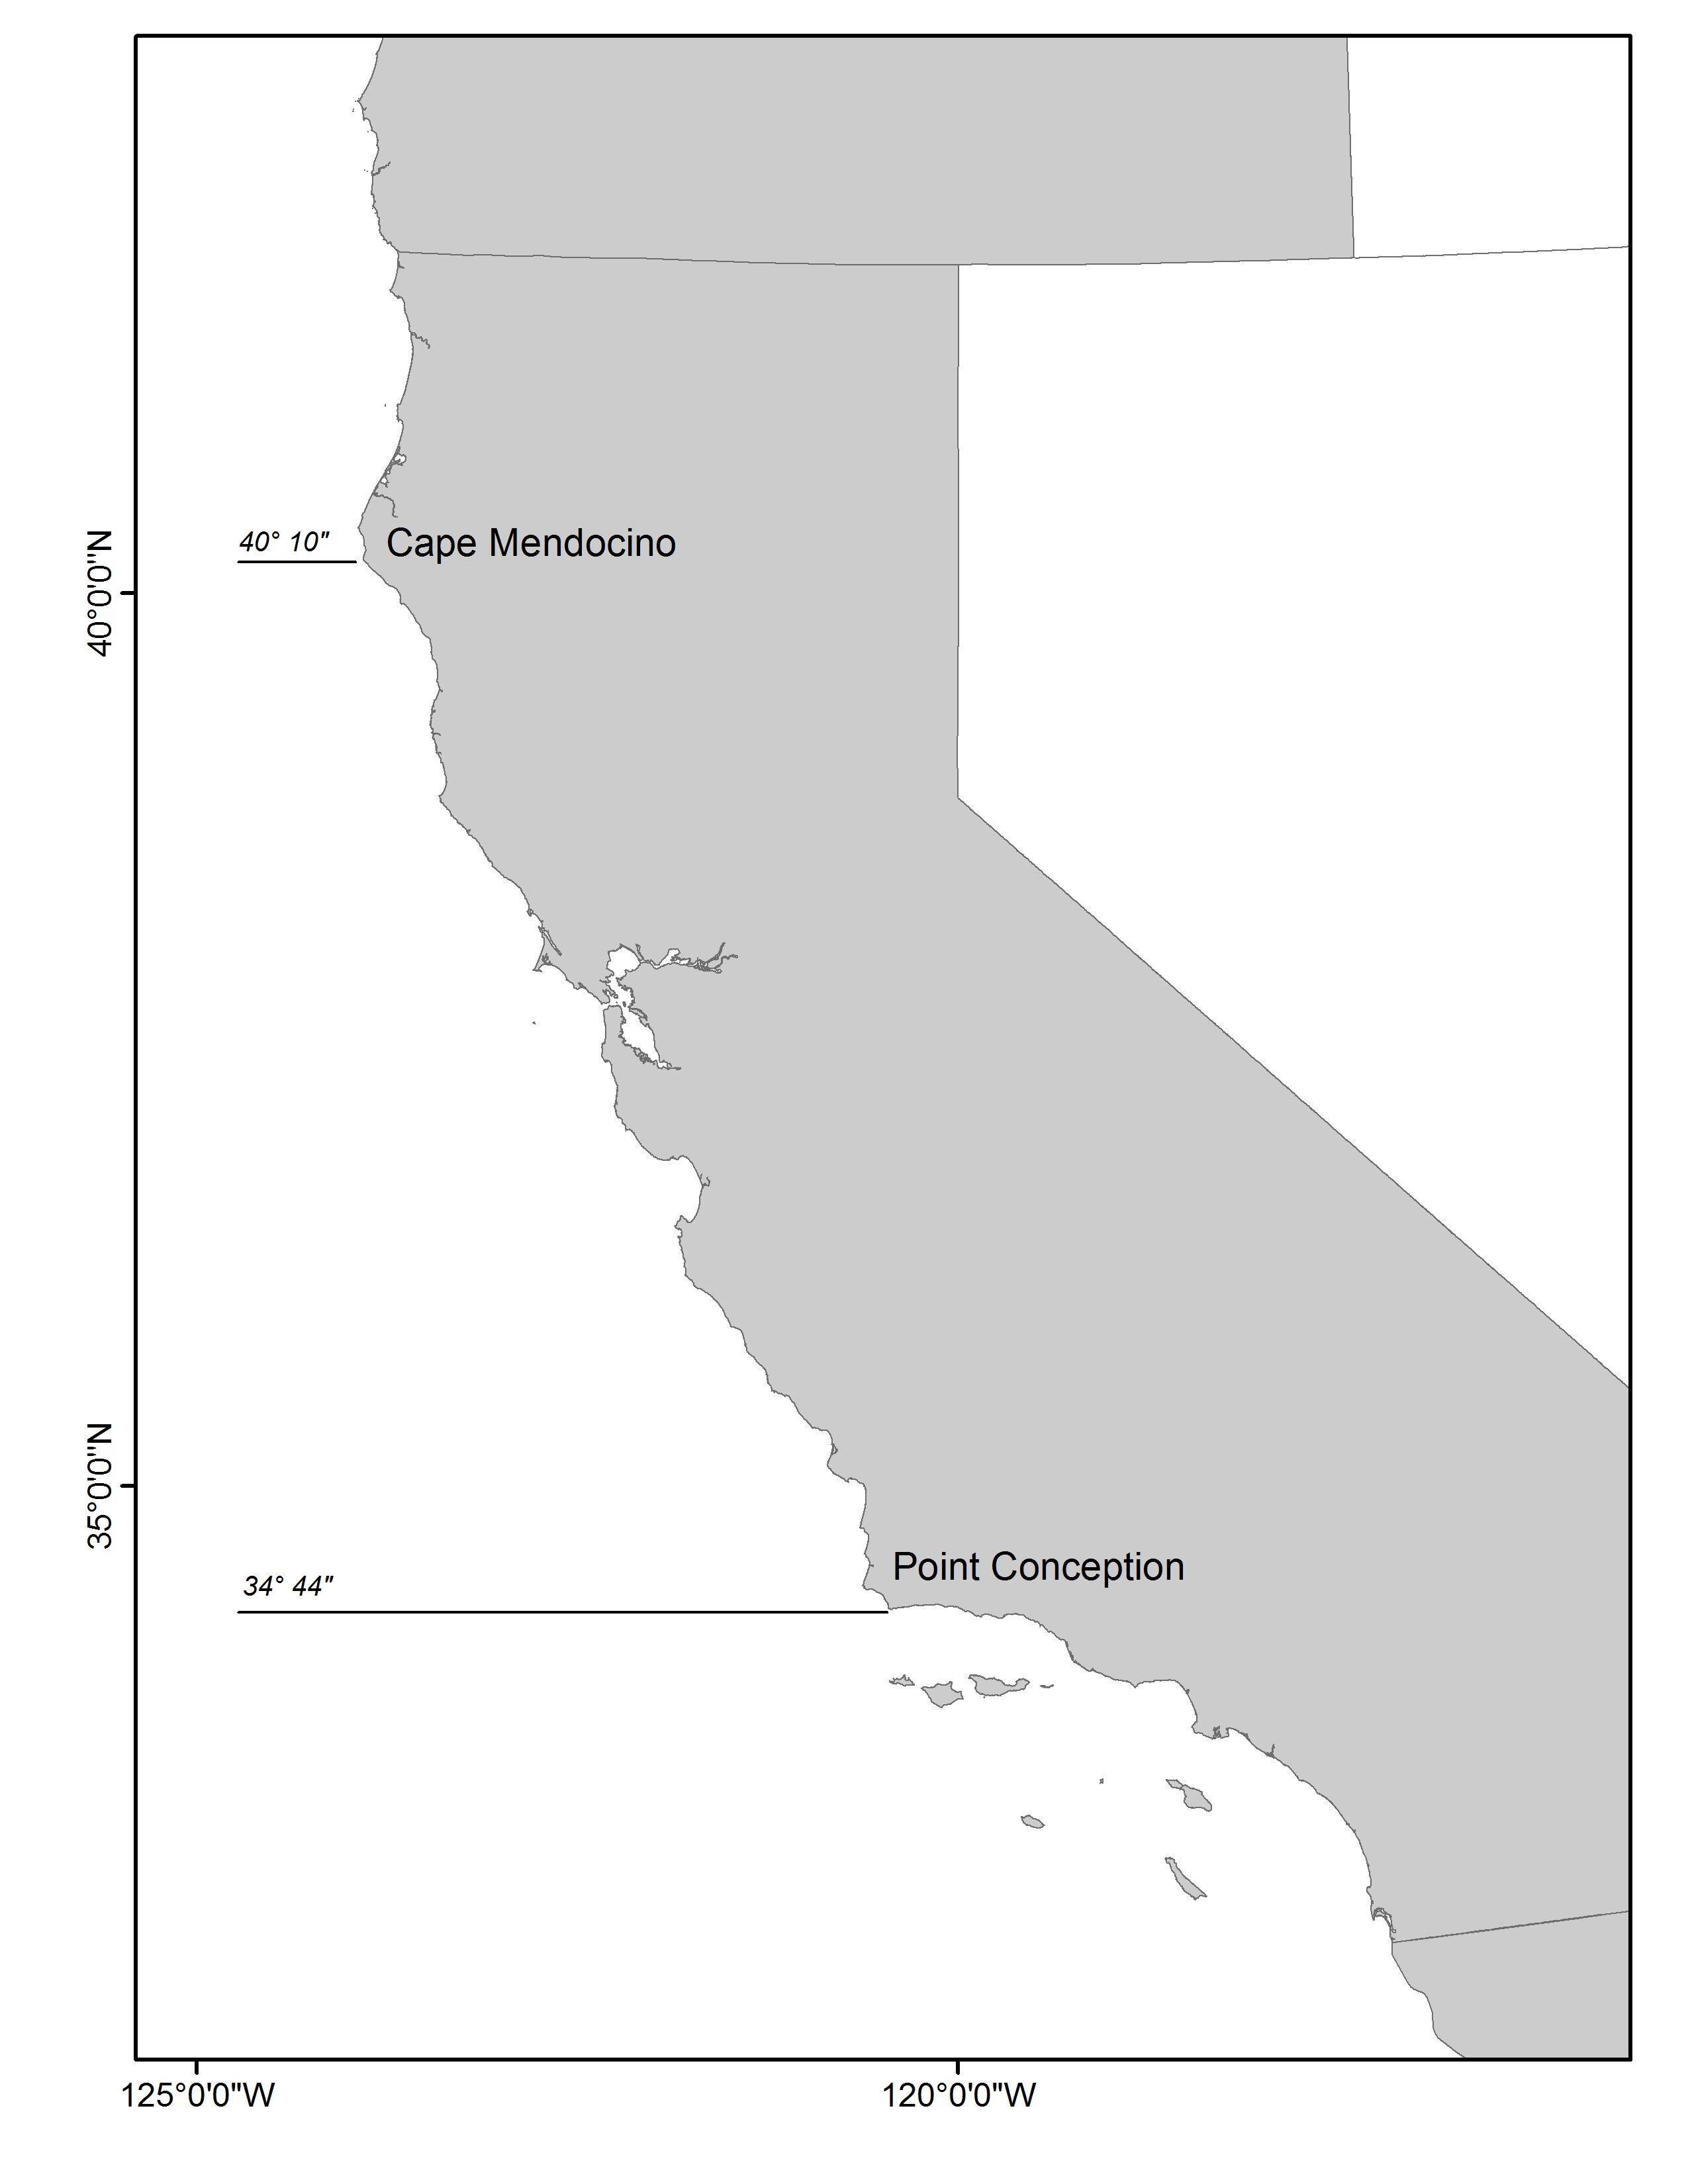
\includegraphics{Figures/assess_region_map.png}
\caption{Map showing the management area for gopher and black-and-yellow
rockfish from Cape Mendocino to the U.S. Mexico
border.\{fig:assess\_reagion\_map\}}
\end{figure}

\begin{figure}
\centering
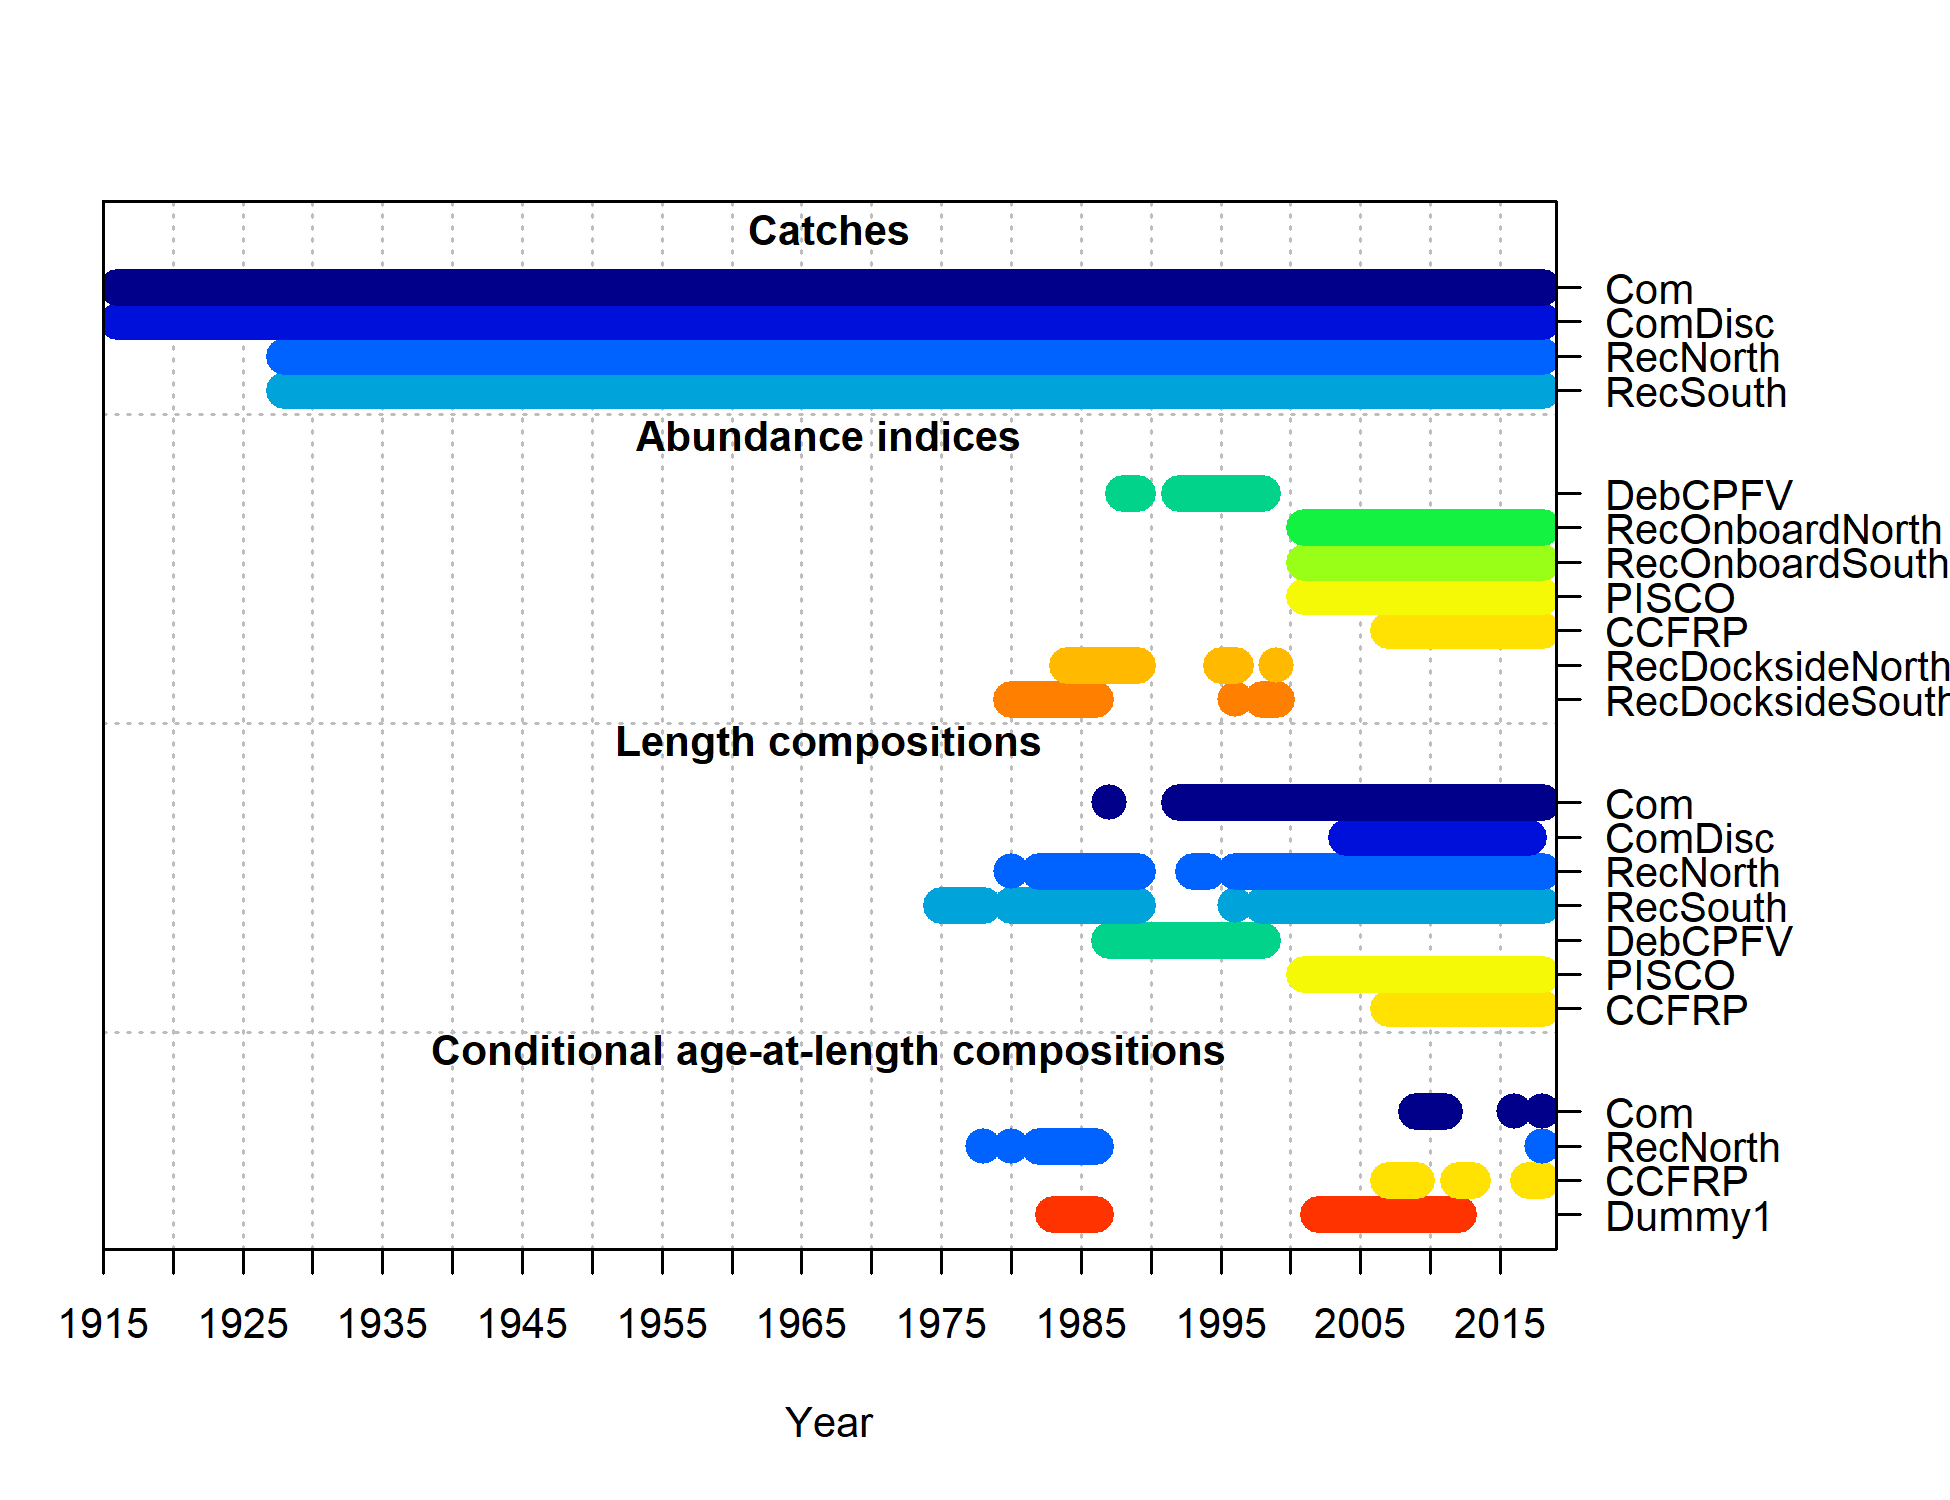
\includegraphics{r4ss/plots_mod1/data_plot.png}
\caption{Summary of data sources used in the model.
\label{fig:data_plot}}
\end{figure}

\begin{figure}
\centering
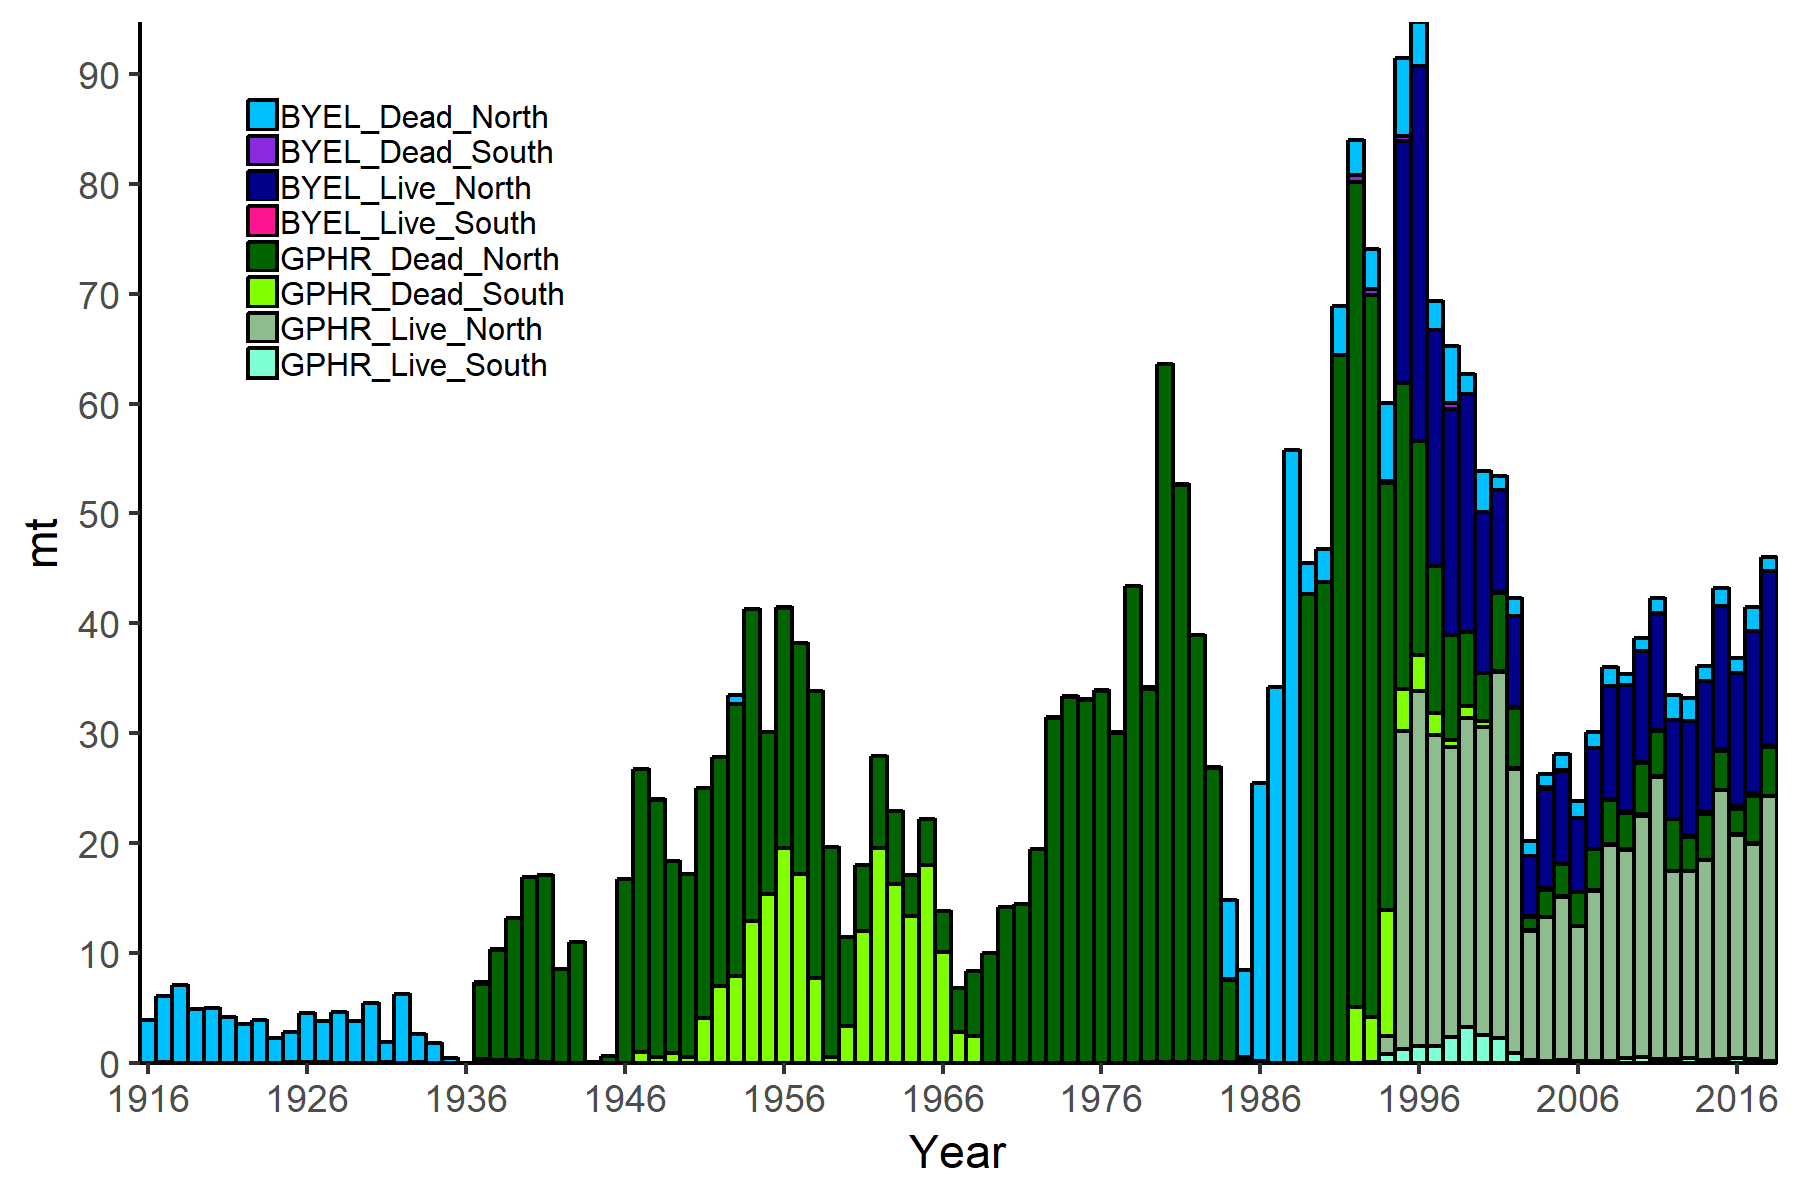
\includegraphics{Figures/Catches_livedeadNS_gby.png}
\caption{Commercial landings for gopher (GPHR) and black-and-yellow
(BYEL) rockfishes landed live and dead north and south of Pt.
Conception. All catch time series were combined for the assessment into
one commercial fleet. \label{fig:Catches_livedeadNS_gby}}
\end{figure}

\begin{figure}
\centering
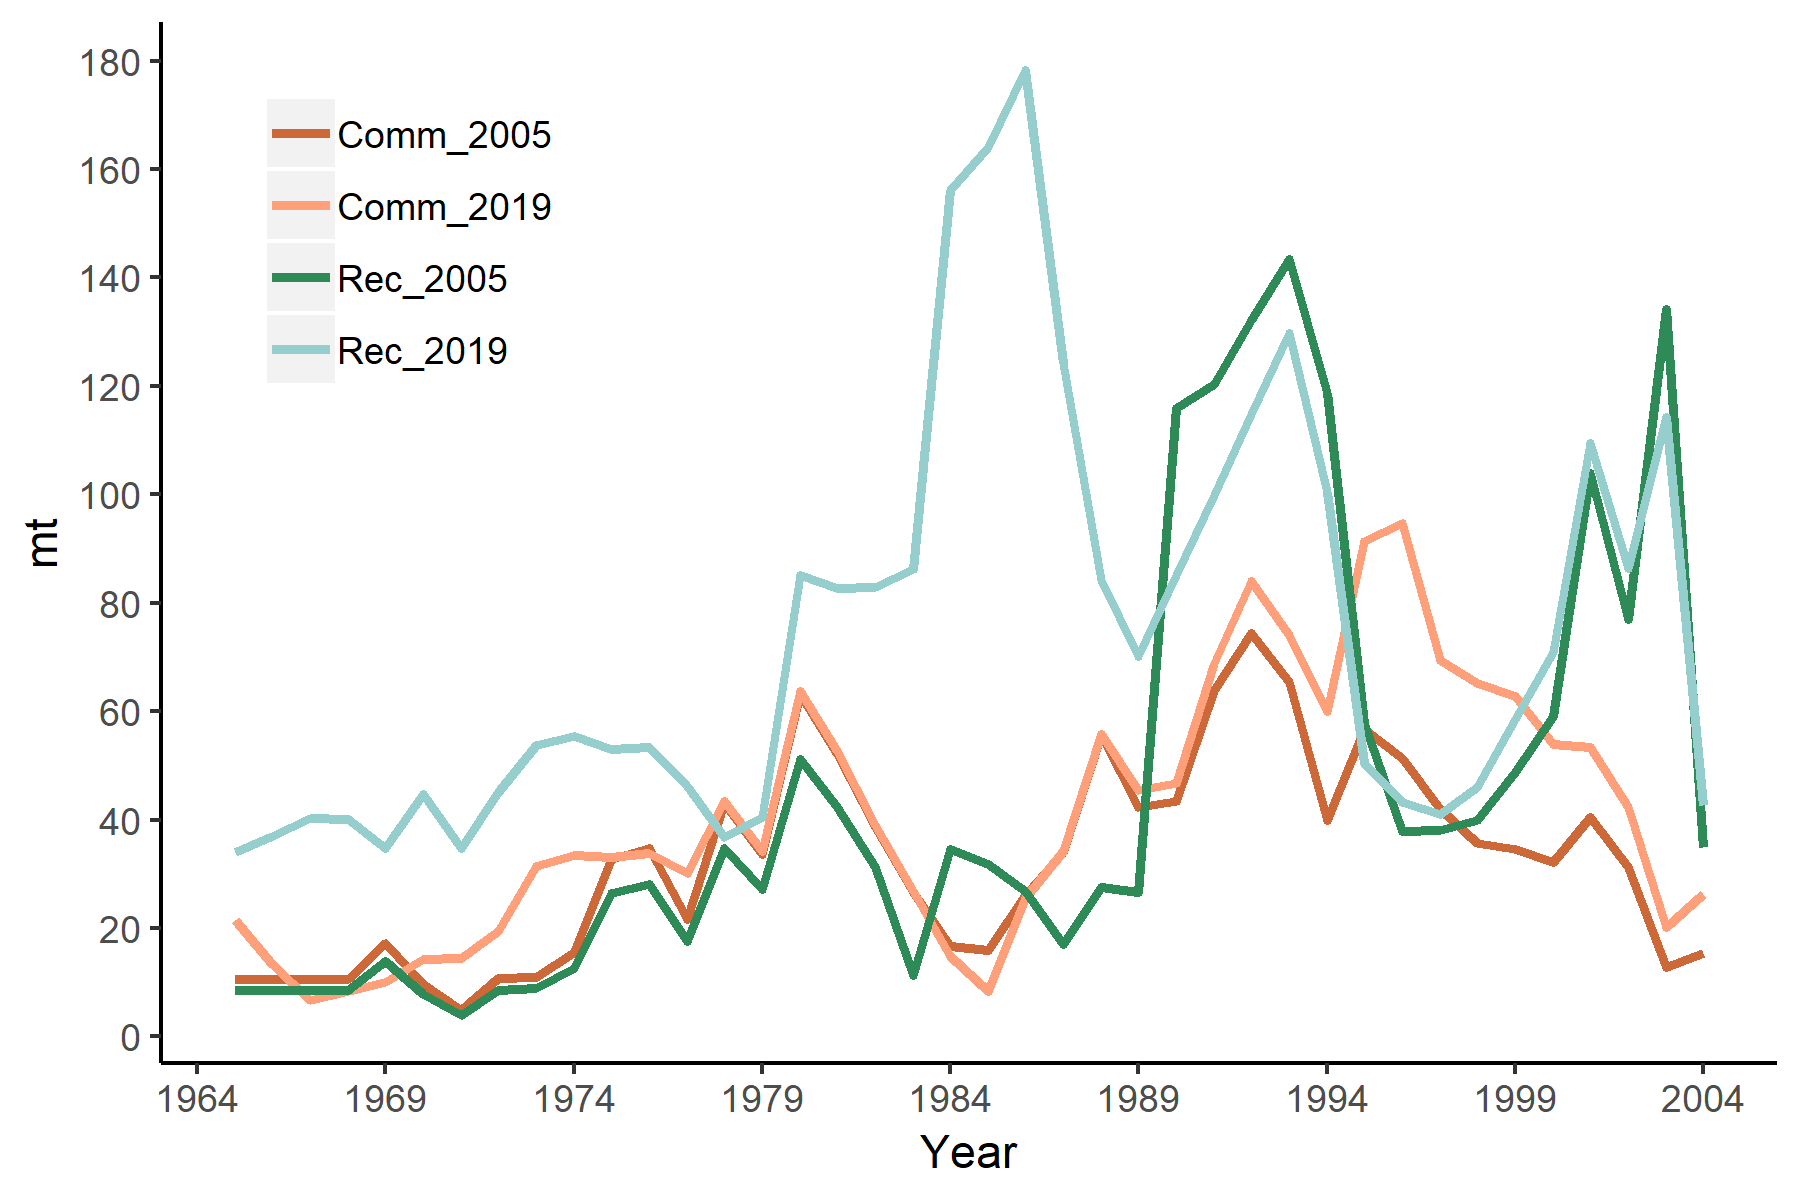
\includegraphics{Figures/assessment_compare.png}
\caption{Comparison of the recreational and commercial fishery landings
from the 2005 assessment to this 2019 assessment. Note that the 2019
assessment includes both gopher and black-and-yellow rockfish where the
2005 assessment represents gopher rockfish only. The 2005 assessment
also did not include landings from south of Pt. Conception.
\label{fig:Assessment_compare}}
\end{figure}

\begin{figure}
\centering
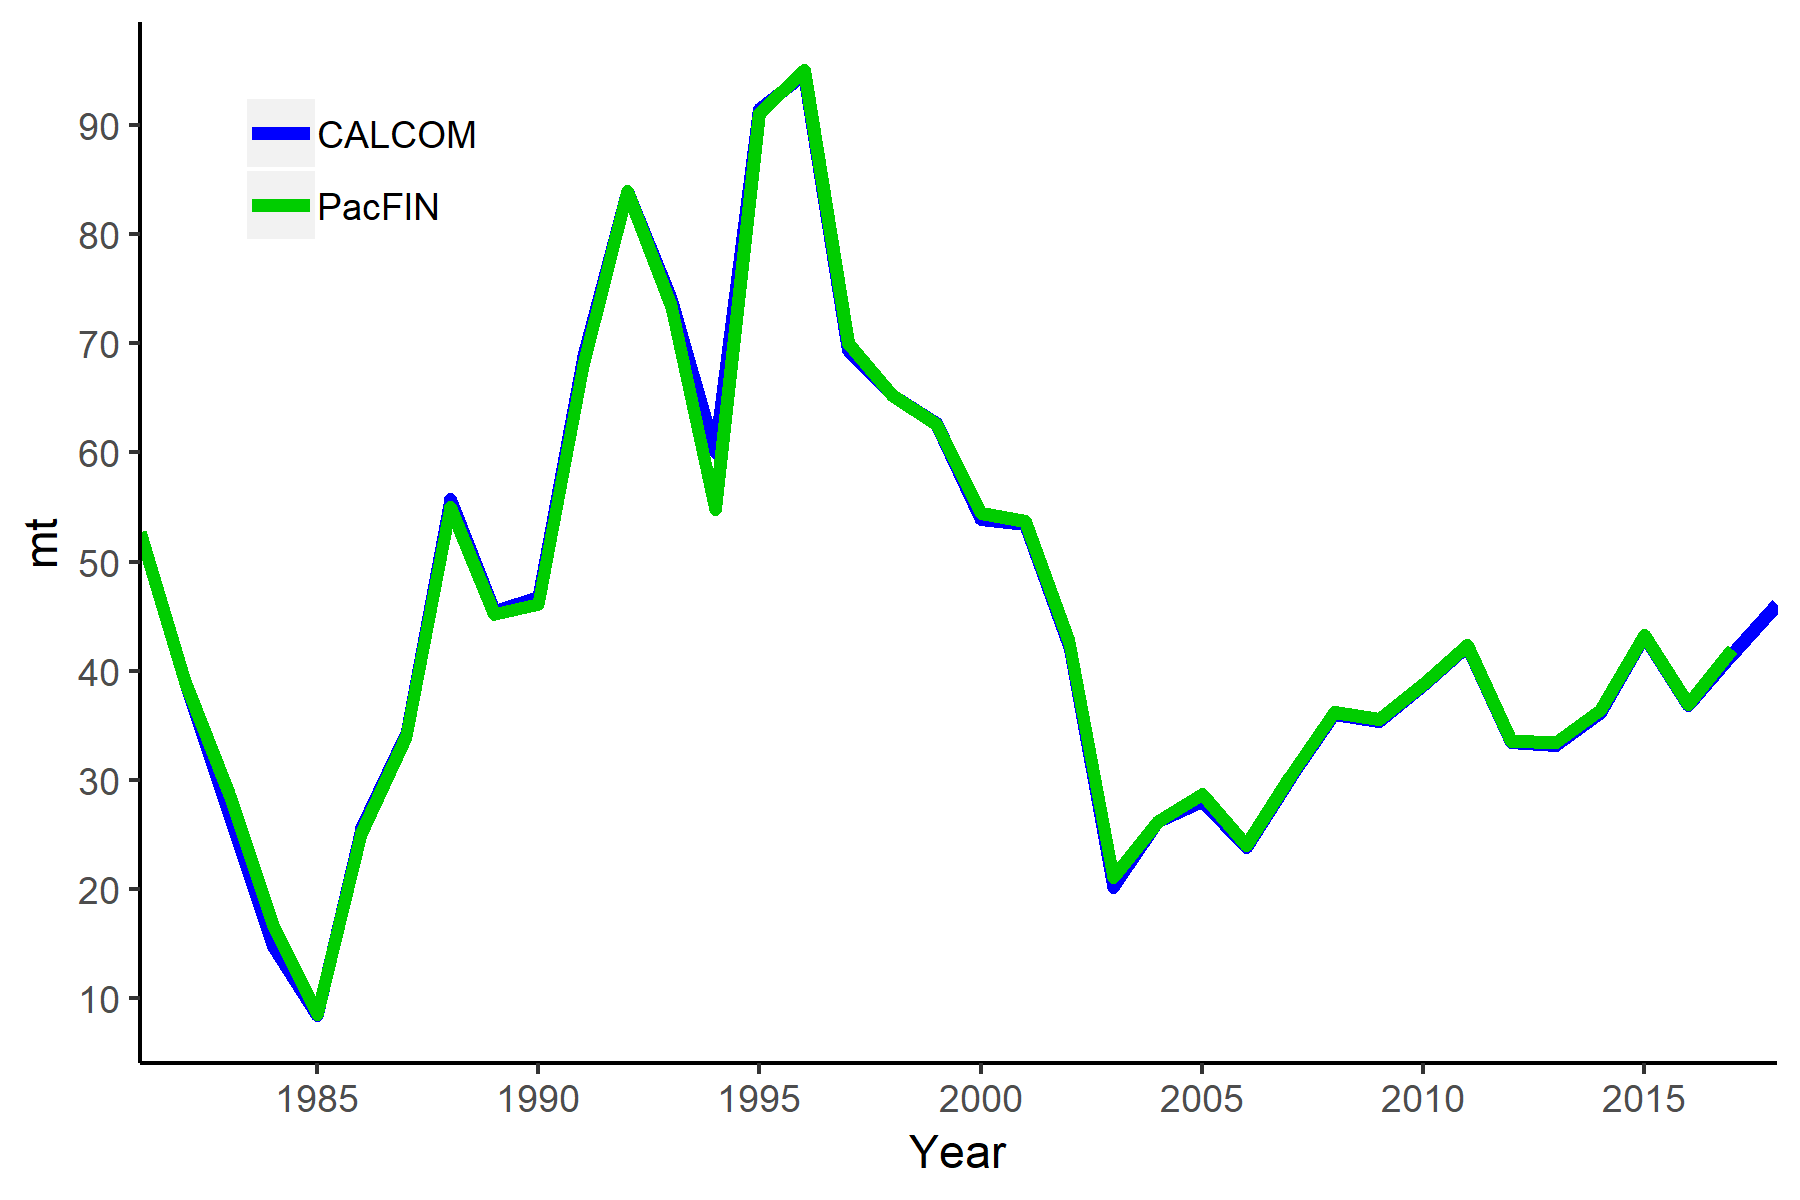
\includegraphics{Figures/Calcom_vs_Pacfin.png}
\caption{Commercial landings estimates from CALCOM add PacFIN.
\label{fig:Calcom_vs_Pacfin}}
\end{figure}

\begin{figure}
\centering
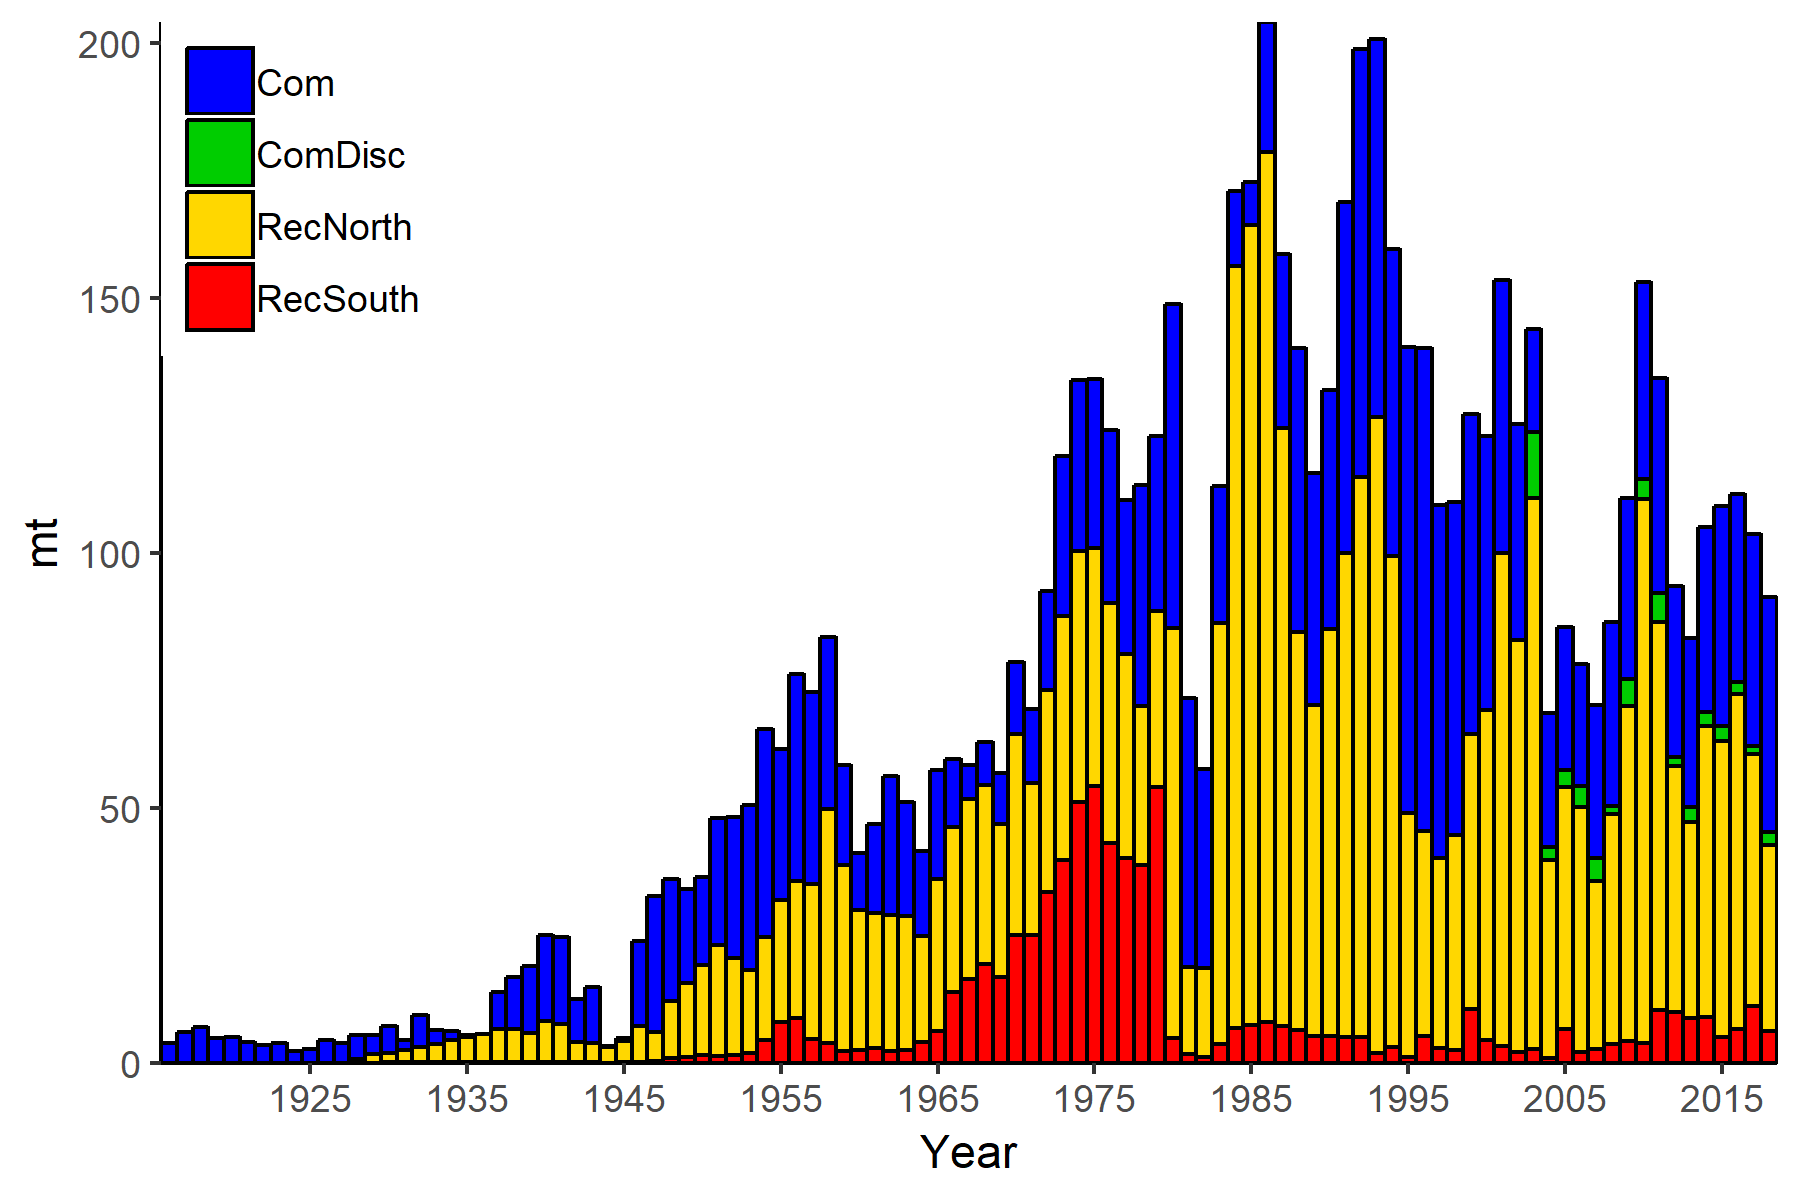
\includegraphics{Figures/Catches_original.png}
\caption{Commercial and recreational landings estimates prior to any
data modification or interpolation to the recreational catches or
hindcasting of commercial discards. \label{fig:Catches_original}}
\end{figure}

\begin{figure}
\centering
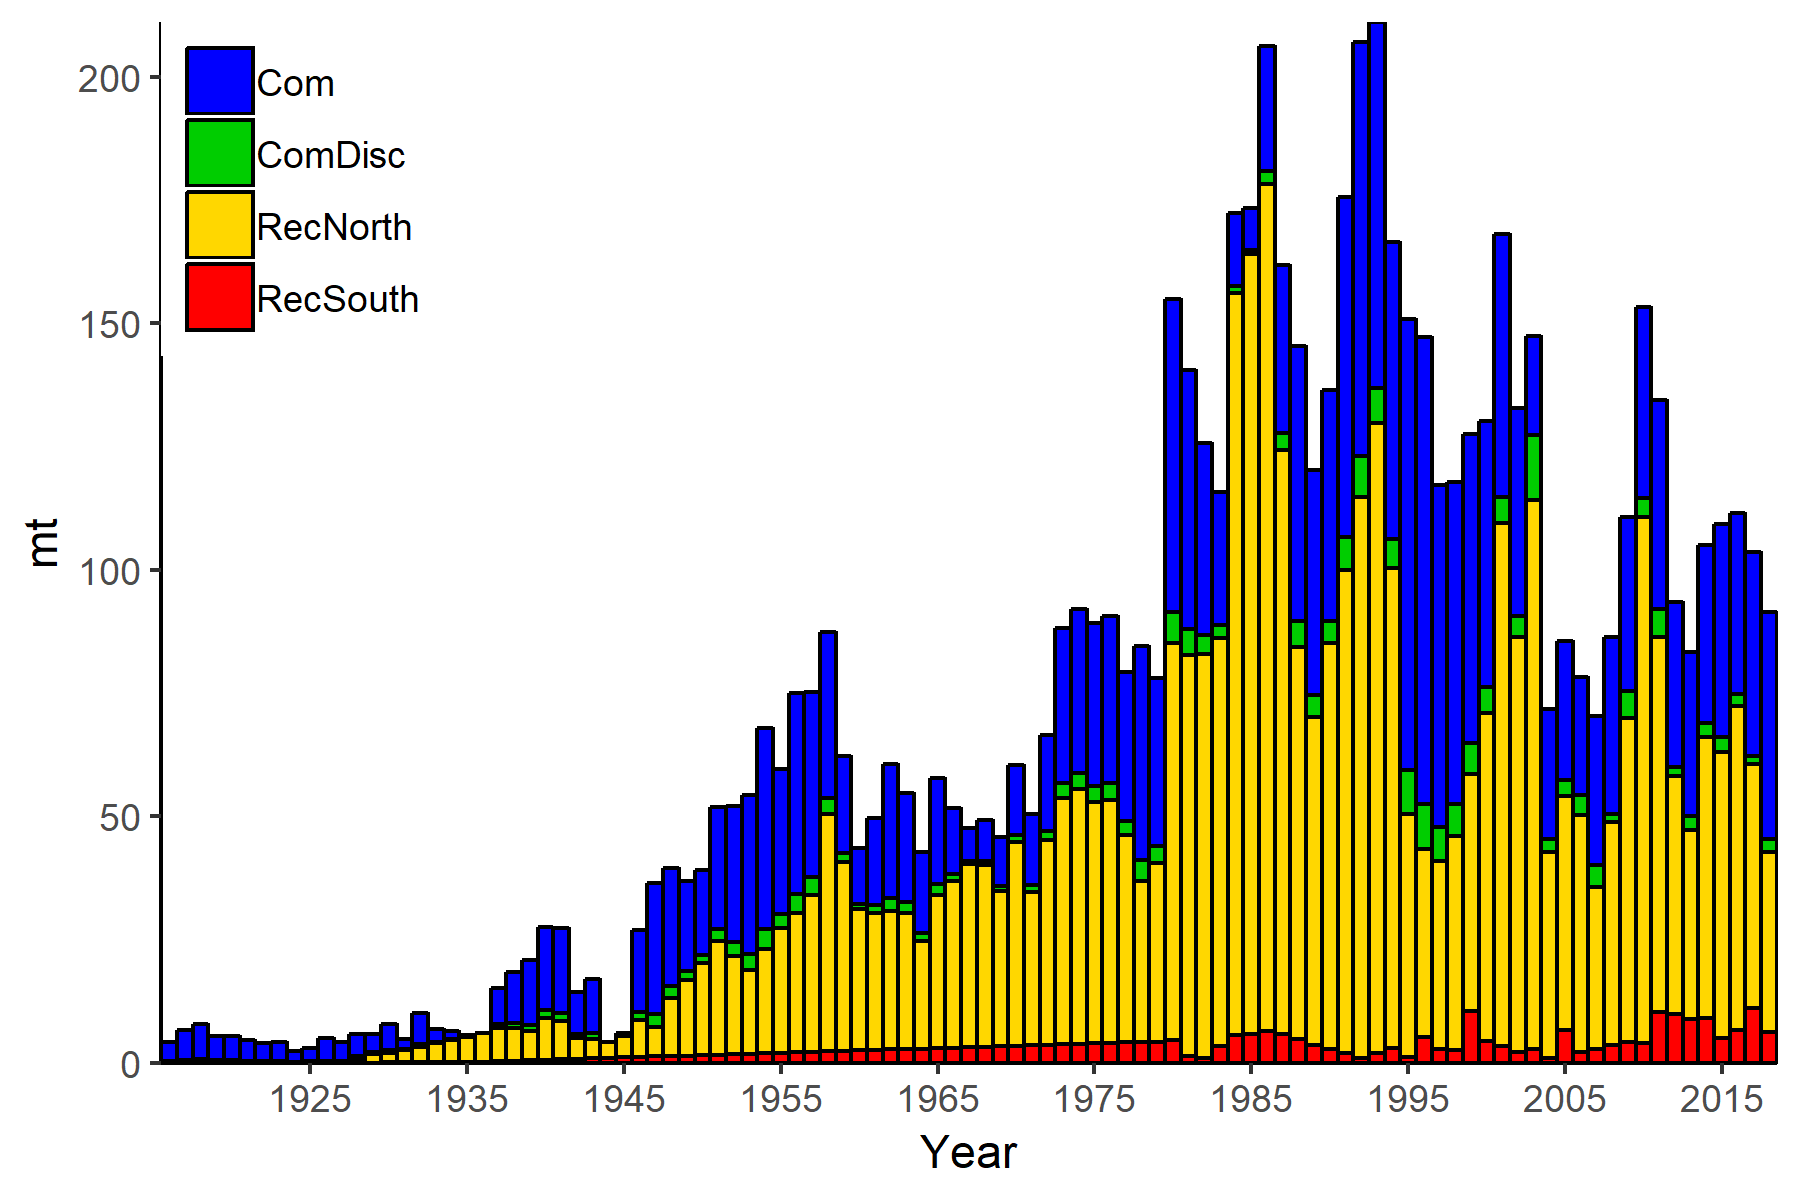
\includegraphics{Figures/Catches_alternate.png}
\caption{Commercial and recreational landings estimates after data
modification and interpolations were made to the recreational catches
and commercial discards. \label{fig:Catches_alternate}}
\end{figure}

\FloatBarrier

\FloatBarrier

\FloatBarrier
<!-- ********************************************************************** -->

\FloatBarrier

\FloatBarrier

\FloatBarrier

\FloatBarrier

\newpage

\color{black}

\section*{References}\label{references}
\addcontentsline{toc}{section}{References}

\renewcommand{\thepage}{}

\hypertarget{refs}{}
\hypertarget{ref-Ally1991}{}
Ally, J., Ono, D., Read, R.B., and Wallace, M. 1991. Status of major
southern California marine sport fish species with management
recommendations, based on analyses of catch and size composition data
collected on board commercial passenger fishing vessels from 1985
through 1987. Marine Resources Division Administrative Report No. 90-2.

\hypertarget{ref-vonB1938}{}
Bertalanffy, L. von. 1938. A quantitative theory of organic growth.
Human Biology \textbf{10}: 181--213.

\hypertarget{ref-Collins1978}{}
Collins, R., and Crooke, S. (n.d.). An evaluation of the commercial
passenger fishing vessel record system and the results of sampling the
Southern California catch for species and size composition, 1975-1978.
Unpublished report.

\hypertarget{ref-Hamel2015}{}
Hamel, O. 2015. A method for calculating a meta-analytical prior for the
natural mortality rate using multiple life history correlates. ICES
Journal of Marine Science \textbf{72}: 62--69.

\hypertarget{ref-Karpov1995}{}
Karpov, K.A., Albin, D.P., and Van Buskirk, W. 1995. The marine
recreational fishery in northern California and central California: a
historical comparison (1958--86), status of stocks (1980--1986), and
effects of changes in the California Current. California Department of
Fish Game Fish Bulletin \textbf{176}.

\hypertarget{ref-PSMFC2018}{}
Pacific Fishery Managment Council. 2018. Status of the Pacific Coast
Groundfish Fishery: Stock Assessment and Fishery Evaluation.

\hypertarget{ref-Pearson2008}{}
Pearson, D.E., Erwin, B., and Key, M. 2008. Reliability of California's
groundfish landings estimates from 1969-2006. NOAA Technical Memorandum
NMFS \textbf{NOAA-TM-NM}.

\hypertarget{ref-Ralston2010}{}
Ralston, S., Pearson, D., Field, J., and Key, M. 2010. Documentation of
California catch reconstruction project. NOAA-TM-NMFS-SWFSC-461.

\hypertarget{ref-Somers2018}{}
Somers, K.A., J. Jannot, V. Tuttle, K. Richerson, N.R., and McVeigh, J.
2018. Estimated discard and catch of groundfish species in the 2017 US
west coast fisheries.. NOAA Fisheries, NWFSC Observer Program, 2725
Montlake Blvd E., Seattle, WA 98112.

\end{document}
